\documentclass[10pt,a4j,dvipdfmx]{jsarticle}
\usepackage[utf8]{inputenc}
\usepackage[dvipdfmx]{graphicx}
\usepackage[usenames,dvipdfmx]{color}
\usepackage{amsmath}
\usepackage{bm}
\usepackage[left=19.05mm, right=19.05mm, top=25.40mm, bottom=25.40mm]{geometry}
\usepackage{tikz}
\usepackage{circuitikz}
\usepackage{siunitx}
\usepackage{listings}
\usepackage{float}
\usepackage{hyperref}
\usepackage{textcomp}
\usepackage{gnuplot-lua-tikz}

\lstset{%
  language={C},
  basicstyle={\small},%
  identifierstyle={\small},%
  commentstyle={\small\itshape},%
  keywordstyle={\small\bfseries},%
  ndkeywordstyle={\small},%
  stringstyle={\small\ttfamily},
  frame={tb},
  breaklines=true,
  columns=[l]{fullflexible},%
  numbers=left,%
  xrightmargin=0zw,%
  xleftmargin=3zw,%
  numberstyle={\scriptsize},%
  stepnumber=1,
  numbersep=1zw,%
  lineskip=-0.5ex%
}

\usepackage{fouriernc}
\usepackage[scaled]{helvet}
\usepackage[T1]{fontenc}
\renewcommand{\ttdefault}{fvm}

\let\oldthefootnote\thefootnote
\def\thefootnote{{\color{Magenta}\oldthefootnote}}

\newcommand{\enhance}[1]{{\gtfamily\sffamily#1}}
\makeatletter
\def\@jikkenname{}
\def\@jikkennum{}
\def\@reportname{}
\def\@studentnumber{}
\def\@studentname{}
\def\@studentdepartment{}
\def\@friendnames{}
\def\@groupnumber{}
\newcommand{\jikkenset}[2]{\def\@jikkennum{#1}\def\@jikkenname{#2}}
\newcommand{\studentset}[3]{\def\@studentnumber{#1}\def\@studentname{#2}\def\@studentdepartment{#3}}
\newcommand{\reportnameset}[1]{\def\@reportname{#1}}
\newcommand{\friendname}[1]{\def\@friendnames{#1}}
\newcommand{\groupnumber}[1]{\def\@groupnumber{#1}}
\renewcommand{\maketitle}{
\noindent{\color{RoyalPurple}\hrule height 1pt \hfill}
\vspace{5pt}
\begin{center}
\enhance{{\Large{電気電子情報一(前期)実験}}}\\[7pt]
\enhance{{\Huge\textbf{\@jikkennum{}. \@jikkenname}}}\\[5pt]
\enhance{{\LARGE{\@reportname}}}\\[15pt]
\@studentnumber\ \ \ \@studentname{}(\@studentdepartment{})\\[1pt]
共同実験者: \@friendnames(第\@groupnumber{}班)\\[1pt]
\today
\end{center}
\vspace{-10pt}
\noindent{\color{RoyalPurple}\hrule height 1pt \hfill}
}
\makeatother
\jikkenset{A3}{ディジタル回路}
\reportnameset{総合レポート}
\studentset{03-160441}{土屋潤一郎}{工学部 電子情報工学科}
\friendname{井上友貴、田中大幹、坂口達彦}
\groupnumber{28}

\makeatletter
\let\@oldsec\section
\let\@oldsubsec\subsection
\renewcommand{\section}[1]{\@oldsec{#1}\vspace{-5pt}{\color{TealBlue}\hrule height 0.6pt \hfill}\par}
\renewcommand{\thesection}{\arabic{section}.}
\renewcommand{\subsection}[1]{\vspace{-7pt}\@oldsubsec{#1}}
\makeatother

\begin{document}
\maketitle

\section{実験の目的}
アナログ回路で出来ているにも関わらず、論理ゲートそれ自体はディジタル回路の中では理想的なディジタル素子として扱える。
その理由を、論理ゲートのパッケージであるICを用いて論理ゲートの基本特性を測定することで理解する。
その上で、簡単な組み合わせ回路や順序回路を設計し、製作して、ディジタル回路の設計について学ぶ。
\section{実験の原理}
\subsection{CMOSインバータ}
CMOSによるNOTゲートは図1のようになる。
入力がHiならば$p$MOSは導通せず、従って電源電圧は出力に伝わらない。
入力がLowならば$p$MOSは導通し、$n$MOSが導通しないので電源電圧がダイレクトに出力となる。
これらCMOSは、TTL等に比べればディジタル素子として理想的であり、基本的なアナログ的な特性としては直流特性とスイッチング特性を知りたい。
直流特性とは、直流電圧に対する出力電圧の特性であり、スイッチング特性とは、スイッチングが実際には即時に行われないことによってアナログ的要素として発生する、Hi/Lowの遷移時間や、入力のスイッチングに対して出力のスイッチングが即時に行われないことによる立ち上がり・立ち下がり時間の特性のことを指す。
\begin{figure}[H]
       \centering
       \includegraphics[width=8cm]{NOT.png}
       \caption{CMOSインバータ}
\end{figure}
 
\subsection{エッジ・トリガD-FF}
ポジティブ・エッジトリガD-FFはクロックと入力d、出力qを持ち、クロック立ち上がり時の入力dを出力qに(1クロックの間)保持し続ける。
その論理ゲートによる構成は図2に示す。

\begin{figure}[H]
       \centering
       \includegraphics[width=12cm]{D-FF.png}
       \caption{ポジティブエッジトリガD-FF}
\end{figure}

\subsection{加算器}
繰り上がりを考慮した1bit1分に足し算を行う回路を全加算器と称す。
2入力x,yに加え入力として前の桁からの繰り上がり$c_in$を持ち、出力としてその桁の結果sとともに次の位への繰り上がり$c_out$を持つ。これを図3に示す。

\begin{figure}[H]
       \centering
       \includegraphics[width=9cm]{FA.png}
       \caption{全加算器}
\end{figure}


全加算器を用いて実際に複数ビット(複数桁)の加算を行う方法はいくつか存在する。
例えば、全加算器を桁数分用意し、各桁の$c_out$を直接次の$c_in$に接続していくリプルキャリーアダーや、桁上がりを先んじて計算しておくキャリールックアヘッドジェネレータを用いた方法などがあるが、これらはいずれも順序回路ではない。

一方、直列加算回路は、一つの全加算器を、記憶素子を組み合わせて使いまわす回路である。その一例を図4に示す。2つのシフトレジスタにそれぞれ足す2進数を入れ、その後スイッチを切り替えてクロックを進めると片方のシフトレジスタに答えが下の桁から入っていく、ということになる。

\begin{figure}[H]
       \centering
       \includegraphics[width=16cm]{token.png}
       \caption{直列加算回路}
\end{figure}

\section{実験方法}
回路の製作はブレッドボード上で行った。
\subsection{CMOSインバータの入出力特性}
図5のような回路を用いて、CMOSインバータの入出力特性を測定する。

\begin{figure}[H]
       \centering
       \includegraphics[width=12cm]{invSokutei.png}
       \caption{CMOSインバータ特性測定回路}
\end{figure}

\subsubsection{閾値電圧の測定}
電源電圧を定格電圧以下で変化させ、それに対する閾値電圧を測定する。
パルスジェネレータは正弦波に設定する。
オシロスコープを特にX-Yモードに設定し、直流特性を測定する。
\subsubsection{立ち上がり時間・立ち下がり時間の測定}
電源電圧と入力電圧を\SI{5}{\volt}に固定し、入力波と負荷のインバータの個数を表1のように変化させ、立ち上がり時間と立ち下がり時間を測定する。

\begin{table}
  \begin{center}
    \caption{立ち上がり時間と立ち下がり時間測定の条件}
    \begin{tabular}{|c|c|c|c|} \hline
      波形 & 周波数[\si{\hertz}] & インバータ数 \\ \hline \hline
      正弦波 & 10k & 3 \\
      正弦波 & 20k & 3 \\
      正弦波 & 50k & 3 \\
      正弦波 & 100k & 3 \\
      正弦波 & 200k & 3 \\
      正弦波 & 500k & 3 \\
      正弦波 & 1M & 3 \\
      正弦波 & 2M & 3 \\
      正弦波 & 5M & 3 \\
      方形波 & 1M & 4 \\             
      方形波 & 1M & 3 \\
      方形波 & 1M & 2 \\
      方形波 & 1M & 1 \\
      \hline
    \end{tabular}
  \end{center}
\end{table}

\subsection{エッヂ・トリガD-FFの構成と動作確認}
図2に示すようなD-FFを構成し、入力dをスイッチング出来るようにし、出力qをその動作を以下の手順で確認する。(0が\SI{0}{\volt}、1が\SI{5}{\volt}である。)

\begin{enumerate}
\item 入力dを1にして、clkを$0\to1$
\item dを適当に変化させる
\item clkを$1\to0$
\item dを適当に変化させる
\item dが0の時、clkを$0\to1$
\item dを適当に変化させる
\item clkを$0\to1$
\item dを適当に変化させる
\end{enumerate}

\subsection{直列加算回路の製作}
\subsubsection{製作と動作確認}
図4のような直列加算回路を製作し、その動作が正しいことを確認する。
\subsubsection{直列加算回路の制御部の設計}
図6のようなタイムチャートを実現する回路を製作し、スタートスイッチを立ち上げてクロックを進めると、8クロックだけenable信号を立ち上げ、図4の回路が8ビット同士の加算を行って停止するような制御を行う。

\begin{figure}[H]
       \centering
       \includegraphics[width=9cm]{token.png}
       \caption{制御回路タイミングチャート}
\end{figure}


\section{使用器具}
\begin{description}
\item[ファンクション・ジェネレータ] IWATSU SG-4104
\item[直流電源] KENWOOD PR18-1.2A
\item[オシロスコープ] LeCroy WaveJet 314
\item[抵抗] \SI{10}{\kilo\ohm}, 1/8W, $\pm$5\%, 炭素皮膜抵抗(プルダウン及びプルアップ用)
\item[コンデンサ] \SI{0.1}{\micro\farad}, 積層セラミックコンデンサ(バイパスコンデンサ用)
\item[NOT IC] HD74HC04(特性測定用), HD74LS04
\item[NAND IC] HD74LS00
\item[D-FF IC] HD74HC175(制御回路), HD74LS175(直列加算回路)
\item[OR IC] HD74LS32
\item[XOR IC] HD74LS86
\item[4bit Counter IC] HD74HC393
\item[8bit shift Register IC] HD74LS164
\end{description}

用意されたHCのICの個数が少なかったため、製作した回路のほとんどで消費電力の大きいLSのICを用いざるを得なかった。

\section{実験結果}

\subsection{CMOSインバータの入出力特性}
\subsubsection{閾値電圧の測定}
図7のように(但し、バイパスコンデンサは無し)回路を組み、図8〜図10のような結果となった。
凡例は(入力電圧, 電源電圧)となっている。
\begin{figure}[H]
    \begin{tabular}{cc}
      %---- 最初の図 ---------------------------
      \begin{minipage}[t]{0.45\hsize}
       \centering
       \includegraphics[width=6cm]{invSokutei.png}
       \caption{CMOSインバータ特性測定回路}
      \end{minipage} &
      %---- 2番目の図 --------------------------
      \begin{minipage}[t]{0.45\hsize}
        \centering
        \scalebox{0.6}{\begin{tikzpicture}[gnuplot]
%% generated with GNUPLOT 4.6p4 (Lua 5.1; terminal rev. 99, script rev. 100)
%% 2016年07月31日 03時47分35秒
\path (0.000,0.000) rectangle (12.500,8.750);
\gpcolor{color=gp lt color border}
\gpsetlinetype{gp lt border}
\gpsetlinewidth{1.00}
\draw[gp path] (1.136,0.985)--(1.316,0.985);
\draw[gp path] (11.947,0.985)--(11.767,0.985);
\node[gp node right] at (0.952,0.985) {-1};
\draw[gp path] (1.136,1.910)--(1.316,1.910);
\draw[gp path] (11.947,1.910)--(11.767,1.910);
\node[gp node right] at (0.952,1.910) { 0};
\draw[gp path] (1.136,2.834)--(1.316,2.834);
\draw[gp path] (11.947,2.834)--(11.767,2.834);
\node[gp node right] at (0.952,2.834) { 1};
\draw[gp path] (1.136,3.759)--(1.316,3.759);
\draw[gp path] (11.947,3.759)--(11.767,3.759);
\node[gp node right] at (0.952,3.759) { 2};
\draw[gp path] (1.136,4.683)--(1.316,4.683);
\draw[gp path] (11.947,4.683)--(11.767,4.683);
\node[gp node right] at (0.952,4.683) { 3};
\draw[gp path] (1.136,5.608)--(1.316,5.608);
\draw[gp path] (11.947,5.608)--(11.767,5.608);
\node[gp node right] at (0.952,5.608) { 4};
\draw[gp path] (1.136,6.532)--(1.316,6.532);
\draw[gp path] (11.947,6.532)--(11.767,6.532);
\node[gp node right] at (0.952,6.532) { 5};
\draw[gp path] (1.136,7.457)--(1.316,7.457);
\draw[gp path] (11.947,7.457)--(11.767,7.457);
\node[gp node right] at (0.952,7.457) { 6};
\draw[gp path] (1.136,8.381)--(1.316,8.381);
\draw[gp path] (11.947,8.381)--(11.767,8.381);
\node[gp node right] at (0.952,8.381) { 7};
\draw[gp path] (1.136,0.985)--(1.136,1.165);
\draw[gp path] (1.136,8.381)--(1.136,8.201);
\node[gp node center] at (1.136,0.677) {-1};
\draw[gp path] (2.487,0.985)--(2.487,1.165);
\draw[gp path] (2.487,8.381)--(2.487,8.201);
\node[gp node center] at (2.487,0.677) { 0};
\draw[gp path] (3.839,0.985)--(3.839,1.165);
\draw[gp path] (3.839,8.381)--(3.839,8.201);
\node[gp node center] at (3.839,0.677) { 1};
\draw[gp path] (5.190,0.985)--(5.190,1.165);
\draw[gp path] (5.190,8.381)--(5.190,8.201);
\node[gp node center] at (5.190,0.677) { 2};
\draw[gp path] (6.542,0.985)--(6.542,1.165);
\draw[gp path] (6.542,8.381)--(6.542,8.201);
\node[gp node center] at (6.542,0.677) { 3};
\draw[gp path] (7.893,0.985)--(7.893,1.165);
\draw[gp path] (7.893,8.381)--(7.893,8.201);
\node[gp node center] at (7.893,0.677) { 4};
\draw[gp path] (9.244,0.985)--(9.244,1.165);
\draw[gp path] (9.244,8.381)--(9.244,8.201);
\node[gp node center] at (9.244,0.677) { 5};
\draw[gp path] (10.596,0.985)--(10.596,1.165);
\draw[gp path] (10.596,8.381)--(10.596,8.201);
\node[gp node center] at (10.596,0.677) { 6};
\draw[gp path] (11.947,0.985)--(11.947,1.165);
\draw[gp path] (11.947,8.381)--(11.947,8.201);
\node[gp node center] at (11.947,0.677) { 7};
\draw[gp path] (1.136,8.381)--(1.136,0.985)--(11.947,0.985)--(11.947,8.381)--cycle;
\node[gp node center,rotate=-270] at (0.246,4.683) {output[V]};
\node[gp node center] at (6.541,0.215) {input[V]};
\node[gp node right] at (10.479,8.047) {3V, 2.99V};
\gpcolor{color=gp lt color 0}
\gpsetpointsize{4.00}
\gppoint{gp mark 1}{(3.352,4.692)}
\gppoint{gp mark 1}{(3.479,4.711)}
\gppoint{gp mark 1}{(3.563,4.692)}
\gppoint{gp mark 1}{(3.690,4.692)}
\gppoint{gp mark 1}{(3.817,4.692)}
\gppoint{gp mark 1}{(3.920,4.692)}
\gppoint{gp mark 1}{(4.041,4.692)}
\gppoint{gp mark 1}{(4.177,4.692)}
\gppoint{gp mark 1}{(4.298,4.692)}
\gppoint{gp mark 1}{(4.420,4.692)}
\gppoint{gp mark 1}{(4.555,4.840)}
\gppoint{gp mark 1}{(4.744,2.068)}
\gppoint{gp mark 1}{(4.852,2.414)}
\gppoint{gp mark 1}{(4.893,1.910)}
\gppoint{gp mark 1}{(5.041,1.895)}
\gppoint{gp mark 1}{(5.163,1.910)}
\gppoint{gp mark 1}{(5.285,1.910)}
\gppoint{gp mark 1}{(5.393,1.910)}
\gppoint{gp mark 1}{(5.501,1.895)}
\gppoint{gp mark 1}{(5.609,1.895)}
\gppoint{gp mark 1}{(5.731,1.895)}
\gppoint{gp mark 1}{(5.839,1.895)}
\gppoint{gp mark 1}{(5.920,1.895)}
\gppoint{gp mark 1}{(6.001,1.895)}
\gppoint{gp mark 1}{(6.069,1.895)}
\gppoint{gp mark 1}{(6.150,1.910)}
\gppoint{gp mark 1}{(6.244,1.895)}
\gppoint{gp mark 1}{(6.298,1.895)}
\gppoint{gp mark 1}{(6.366,1.895)}
\gppoint{gp mark 1}{(6.393,1.895)}
\gppoint{gp mark 1}{(6.447,1.895)}
\gppoint{gp mark 1}{(6.474,1.895)}
\gppoint{gp mark 1}{(6.487,1.895)}
\gppoint{gp mark 1}{(6.514,1.895)}
\gppoint{gp mark 1}{(6.514,1.895)}
\gppoint{gp mark 1}{(6.542,1.910)}
\gppoint{gp mark 1}{(6.514,1.895)}
\gppoint{gp mark 1}{(6.514,1.910)}
\gppoint{gp mark 1}{(6.487,1.895)}
\gppoint{gp mark 1}{(6.447,1.895)}
\gppoint{gp mark 1}{(6.406,1.910)}
\gppoint{gp mark 1}{(6.366,1.910)}
\gppoint{gp mark 1}{(6.325,1.895)}
\gppoint{gp mark 1}{(6.258,1.895)}
\gppoint{gp mark 1}{(6.204,1.910)}
\gppoint{gp mark 1}{(6.136,1.895)}
\gppoint{gp mark 1}{(6.055,1.910)}
\gppoint{gp mark 1}{(5.960,1.895)}
\gppoint{gp mark 1}{(5.866,1.910)}
\gppoint{gp mark 1}{(5.771,1.910)}
\gppoint{gp mark 1}{(5.650,1.910)}
\gppoint{gp mark 1}{(5.569,1.910)}
\gppoint{gp mark 1}{(5.433,1.895)}
\gppoint{gp mark 1}{(5.325,1.910)}
\gppoint{gp mark 1}{(5.204,1.910)}
\gppoint{gp mark 1}{(5.096,1.895)}
\gppoint{gp mark 1}{(4.974,1.910)}
\gppoint{gp mark 1}{(4.852,1.910)}
\gppoint{gp mark 1}{(4.717,1.910)}
\gppoint{gp mark 1}{(4.568,1.895)}
\gppoint{gp mark 1}{(4.460,4.942)}
\gppoint{gp mark 1}{(4.339,4.711)}
\gppoint{gp mark 1}{(4.217,4.692)}
\gppoint{gp mark 1}{(4.109,4.711)}
\gppoint{gp mark 1}{(3.974,4.692)}
\gppoint{gp mark 1}{(3.852,4.711)}
\gppoint{gp mark 1}{(3.732,4.711)}
\gppoint{gp mark 1}{(3.606,4.692)}
\gppoint{gp mark 1}{(3.521,4.692)}
\gppoint{gp mark 1}{(3.394,4.692)}
\gppoint{gp mark 1}{(3.289,4.692)}
\gppoint{gp mark 1}{(3.205,4.692)}
\gppoint{gp mark 1}{(3.100,4.692)}
\gppoint{gp mark 1}{(3.014,4.692)}
\gppoint{gp mark 1}{(2.931,4.692)}
\gppoint{gp mark 1}{(2.867,4.711)}
\gppoint{gp mark 1}{(2.782,4.692)}
\gppoint{gp mark 1}{(2.718,4.692)}
\gppoint{gp mark 1}{(2.677,4.692)}
\gppoint{gp mark 1}{(2.635,4.692)}
\gppoint{gp mark 1}{(2.572,4.692)}
\gppoint{gp mark 1}{(2.551,4.692)}
\gppoint{gp mark 1}{(2.530,4.692)}
\gppoint{gp mark 1}{(2.508,4.692)}
\gppoint{gp mark 1}{(2.508,4.692)}
\gppoint{gp mark 1}{(2.508,4.692)}
\gppoint{gp mark 1}{(2.508,4.692)}
\gppoint{gp mark 1}{(2.530,4.692)}
\gppoint{gp mark 1}{(2.530,4.692)}
\gppoint{gp mark 1}{(2.572,4.692)}
\gppoint{gp mark 1}{(2.614,4.692)}
\gppoint{gp mark 1}{(2.656,4.692)}
\gppoint{gp mark 1}{(2.698,4.711)}
\gppoint{gp mark 1}{(2.762,4.692)}
\gppoint{gp mark 1}{(2.825,4.692)}
\gppoint{gp mark 1}{(2.887,4.692)}
\gppoint{gp mark 1}{(2.973,4.692)}
\gppoint{gp mark 1}{(3.056,4.692)}
\gppoint{gp mark 1}{(3.163,4.692)}
\gppoint{gp mark 1}{(3.247,4.692)}
\gppoint{gp mark 1}{(3.352,4.692)}
\gppoint{gp mark 1}{(3.479,4.692)}
\gppoint{gp mark 1}{(3.585,4.692)}
\gppoint{gp mark 1}{(3.690,4.692)}
\gppoint{gp mark 1}{(3.796,4.692)}
\gppoint{gp mark 1}{(3.920,4.683)}
\gppoint{gp mark 1}{(4.041,4.692)}
\gppoint{gp mark 1}{(4.177,4.692)}
\gppoint{gp mark 1}{(4.298,4.692)}
\gppoint{gp mark 1}{(4.420,4.692)}
\gppoint{gp mark 1}{(4.528,4.840)}
\gppoint{gp mark 1}{(4.758,2.169)}
\gppoint{gp mark 1}{(4.987,3.564)}
\gppoint{gp mark 1}{(4.906,1.910)}
\gppoint{gp mark 1}{(5.041,1.895)}
\gppoint{gp mark 1}{(5.163,1.895)}
\gppoint{gp mark 1}{(5.285,1.895)}
\gppoint{gp mark 1}{(5.393,1.895)}
\gppoint{gp mark 1}{(5.501,1.895)}
\gppoint{gp mark 1}{(5.623,1.895)}
\gppoint{gp mark 1}{(5.731,1.895)}
\gppoint{gp mark 1}{(5.839,1.895)}
\gppoint{gp mark 1}{(5.920,1.910)}
\gppoint{gp mark 1}{(6.001,1.895)}
\gppoint{gp mark 1}{(6.096,1.910)}
\gppoint{gp mark 1}{(6.150,1.910)}
\gppoint{gp mark 1}{(6.244,1.910)}
\gppoint{gp mark 1}{(6.298,1.895)}
\gppoint{gp mark 1}{(6.366,1.895)}
\gppoint{gp mark 1}{(6.406,1.895)}
\gppoint{gp mark 1}{(6.433,1.895)}
\gppoint{gp mark 1}{(6.474,1.910)}
\gppoint{gp mark 1}{(6.514,1.895)}
\gppoint{gp mark 1}{(6.514,1.910)}
\gppoint{gp mark 1}{(6.542,1.910)}
\gppoint{gp mark 1}{(6.542,1.895)}
\gppoint{gp mark 1}{(6.542,1.910)}
\gppoint{gp mark 1}{(6.514,1.910)}
\gppoint{gp mark 1}{(6.487,1.895)}
\gppoint{gp mark 1}{(6.447,1.910)}
\gppoint{gp mark 1}{(6.433,1.910)}
\gppoint{gp mark 1}{(6.393,1.895)}
\gppoint{gp mark 1}{(6.325,1.895)}
\gppoint{gp mark 1}{(6.258,1.910)}
\gppoint{gp mark 1}{(6.204,1.910)}
\gppoint{gp mark 1}{(6.109,1.910)}
\gppoint{gp mark 1}{(6.028,1.910)}
\gppoint{gp mark 1}{(5.960,1.895)}
\gppoint{gp mark 1}{(5.866,1.910)}
\gppoint{gp mark 1}{(5.771,1.895)}
\gppoint{gp mark 1}{(5.663,1.910)}
\gppoint{gp mark 1}{(5.541,1.910)}
\gppoint{gp mark 1}{(5.433,1.910)}
\gppoint{gp mark 1}{(5.325,1.910)}
\gppoint{gp mark 1}{(5.204,1.910)}
\gppoint{gp mark 1}{(5.096,1.910)}
\gppoint{gp mark 1}{(4.974,1.910)}
\gppoint{gp mark 1}{(4.852,1.910)}
\gppoint{gp mark 1}{(4.717,1.910)}
\gppoint{gp mark 1}{(4.596,1.910)}
\gppoint{gp mark 1}{(4.420,5.108)}
\gppoint{gp mark 1}{(4.366,4.711)}
\gppoint{gp mark 1}{(4.217,4.711)}
\gppoint{gp mark 1}{(4.082,4.711)}
\gppoint{gp mark 1}{(3.960,4.711)}
\gppoint{gp mark 1}{(3.852,4.711)}
\gppoint{gp mark 1}{(3.732,4.692)}
\gppoint{gp mark 1}{(3.606,4.711)}
\gppoint{gp mark 1}{(3.501,4.711)}
\gppoint{gp mark 1}{(3.394,4.692)}
\gppoint{gp mark 1}{(3.289,4.692)}
\gppoint{gp mark 1}{(3.205,4.711)}
\gppoint{gp mark 1}{(3.100,4.692)}
\gppoint{gp mark 1}{(3.014,4.692)}
\gppoint{gp mark 1}{(2.951,4.692)}
\gppoint{gp mark 1}{(2.845,4.711)}
\gppoint{gp mark 1}{(2.782,4.692)}
\gppoint{gp mark 1}{(2.718,4.692)}
\gppoint{gp mark 1}{(2.677,4.692)}
\gppoint{gp mark 1}{(2.614,4.692)}
\gppoint{gp mark 1}{(2.593,4.692)}
\gppoint{gp mark 1}{(2.551,4.711)}
\gppoint{gp mark 1}{(2.530,4.692)}
\gppoint{gp mark 1}{(2.508,4.692)}
\gppoint{gp mark 1}{(2.508,4.711)}
\gppoint{gp mark 1}{(2.508,4.692)}
\gppoint{gp mark 1}{(2.508,4.692)}
\gppoint{gp mark 1}{(2.530,4.692)}
\gppoint{gp mark 1}{(2.530,4.692)}
\gppoint{gp mark 1}{(2.572,4.692)}
\gppoint{gp mark 1}{(2.614,4.692)}
\gppoint{gp mark 1}{(2.656,4.692)}
\gppoint{gp mark 1}{(2.698,4.692)}
\gppoint{gp mark 1}{(2.762,4.692)}
\gppoint{gp mark 1}{(2.825,4.692)}
\gppoint{gp mark 1}{(2.909,4.692)}
\gppoint{gp mark 1}{(2.994,4.692)}
\gppoint{gp mark 1}{(3.056,4.692)}
\gppoint{gp mark 1}{(3.163,4.692)}
\gppoint{gp mark 1}{(3.247,4.692)}
\gppoint{gp mark 1}{(3.352,4.692)}
\gppoint{gp mark 1}{(3.458,4.692)}
\gppoint{gp mark 1}{(3.585,4.692)}
\gppoint{gp mark 1}{(3.690,4.692)}
\gppoint{gp mark 1}{(3.817,4.692)}
\gppoint{gp mark 1}{(3.920,4.692)}
\gppoint{gp mark 1}{(4.041,4.692)}
\gppoint{gp mark 1}{(4.177,4.692)}
\gppoint{gp mark 1}{(4.298,4.683)}
\gppoint{gp mark 1}{(4.420,4.692)}
\gppoint{gp mark 1}{(4.514,4.581)}
\gppoint{gp mark 1}{(4.555,2.270)}
\gppoint{gp mark 1}{(4.798,1.967)}
\gppoint{gp mark 1}{(4.825,2.256)}
\gppoint{gp mark 1}{(5.014,1.895)}
\gppoint{gp mark 1}{(5.163,1.910)}
\gppoint{gp mark 1}{(5.285,1.895)}
\gppoint{gp mark 1}{(5.393,1.895)}
\gppoint{gp mark 1}{(5.528,1.910)}
\gppoint{gp mark 1}{(5.623,1.895)}
\gppoint{gp mark 1}{(5.731,1.895)}
\gppoint{gp mark 1}{(5.839,1.895)}
\gppoint{gp mark 1}{(5.920,1.895)}
\gppoint{gp mark 1}{(6.001,1.895)}
\gppoint{gp mark 1}{(6.096,1.895)}
\gppoint{gp mark 1}{(6.177,1.895)}
\gppoint{gp mark 1}{(6.244,1.895)}
\gppoint{gp mark 1}{(6.298,1.895)}
\gppoint{gp mark 1}{(6.339,1.895)}
\gppoint{gp mark 1}{(6.406,1.895)}
\gppoint{gp mark 1}{(6.447,1.910)}
\gppoint{gp mark 1}{(6.474,1.910)}
\gppoint{gp mark 1}{(6.514,1.895)}
\gppoint{gp mark 1}{(6.514,1.910)}
\gppoint{gp mark 1}{(6.542,1.895)}
\gppoint{gp mark 1}{(6.542,1.910)}
\gppoint{gp mark 1}{(6.514,1.910)}
\gppoint{gp mark 1}{(6.514,1.910)}
\gppoint{gp mark 1}{(6.474,1.910)}
\gppoint{gp mark 1}{(6.447,1.910)}
\gppoint{gp mark 1}{(6.433,1.910)}
\gppoint{gp mark 1}{(6.366,1.910)}
\gppoint{gp mark 1}{(6.325,1.910)}
\gppoint{gp mark 1}{(6.258,1.910)}
\gppoint{gp mark 1}{(6.204,1.910)}
\gppoint{gp mark 1}{(6.136,1.910)}
\gppoint{gp mark 1}{(6.055,1.895)}
\gppoint{gp mark 1}{(5.960,1.895)}
\gppoint{gp mark 1}{(5.879,1.910)}
\gppoint{gp mark 1}{(5.771,1.910)}
\gppoint{gp mark 1}{(5.663,1.910)}
\gppoint{gp mark 1}{(5.541,1.895)}
\gppoint{gp mark 1}{(5.433,1.910)}
\gppoint{gp mark 1}{(5.325,1.910)}
\gppoint{gp mark 1}{(5.204,1.910)}
\gppoint{gp mark 1}{(5.096,1.895)}
\gppoint{gp mark 1}{(4.974,1.910)}
\gppoint{gp mark 1}{(4.852,1.910)}
\gppoint{gp mark 1}{(4.717,1.910)}
\gppoint{gp mark 1}{(4.596,1.910)}
\gppoint{gp mark 1}{(4.420,5.108)}
\gppoint{gp mark 1}{(4.366,4.711)}
\gppoint{gp mark 1}{(4.217,4.692)}
\gppoint{gp mark 1}{(4.082,4.692)}
\gppoint{gp mark 1}{(3.960,4.692)}
\gppoint{gp mark 1}{(3.852,4.711)}
\gppoint{gp mark 1}{(3.732,4.711)}
\gppoint{gp mark 1}{(3.627,4.692)}
\gppoint{gp mark 1}{(3.501,4.692)}
\gppoint{gp mark 1}{(3.394,4.692)}
\gppoint{gp mark 1}{(3.289,4.711)}
\gppoint{gp mark 1}{(3.205,4.692)}
\gppoint{gp mark 1}{(3.100,4.692)}
\gppoint{gp mark 1}{(3.014,4.692)}
\gppoint{gp mark 1}{(2.931,4.692)}
\gppoint{gp mark 1}{(2.867,4.692)}
\gppoint{gp mark 1}{(2.782,4.711)}
\gppoint{gp mark 1}{(2.740,4.692)}
\gppoint{gp mark 1}{(2.656,4.692)}
\gppoint{gp mark 1}{(2.635,4.692)}
\gppoint{gp mark 1}{(2.593,4.692)}
\gppoint{gp mark 1}{(2.551,4.692)}
\gppoint{gp mark 1}{(2.530,4.692)}
\gppoint{gp mark 1}{(2.508,4.692)}
\gppoint{gp mark 1}{(2.508,4.692)}
\gppoint{gp mark 1}{(2.508,4.692)}
\gppoint{gp mark 1}{(2.508,4.692)}
\gppoint{gp mark 1}{(2.530,4.692)}
\gppoint{gp mark 1}{(2.551,4.692)}
\gppoint{gp mark 1}{(2.572,4.692)}
\gppoint{gp mark 1}{(2.614,4.692)}
\gppoint{gp mark 1}{(2.656,4.692)}
\gppoint{gp mark 1}{(2.698,4.692)}
\gppoint{gp mark 1}{(2.762,4.692)}
\gppoint{gp mark 1}{(2.825,4.692)}
\gppoint{gp mark 1}{(2.887,4.692)}
\gppoint{gp mark 1}{(2.994,4.692)}
\gppoint{gp mark 1}{(3.056,4.692)}
\gppoint{gp mark 1}{(3.163,4.692)}
\gppoint{gp mark 1}{(3.247,4.692)}
\gppoint{gp mark 1}{(3.352,4.692)}
\gppoint{gp mark 1}{(3.458,4.692)}
\gppoint{gp mark 1}{(3.585,4.692)}
\gppoint{gp mark 1}{(3.690,4.692)}
\gppoint{gp mark 1}{(3.817,4.692)}
\gppoint{gp mark 1}{(3.920,4.692)}
\gppoint{gp mark 1}{(4.041,4.692)}
\gppoint{gp mark 1}{(4.177,4.692)}
\gppoint{gp mark 1}{(4.298,4.692)}
\gppoint{gp mark 1}{(4.420,4.692)}
\gppoint{gp mark 1}{(4.514,4.720)}
\gppoint{gp mark 1}{(4.758,2.141)}
\gppoint{gp mark 1}{(4.974,3.324)}
\gppoint{gp mark 1}{(4.906,1.910)}
\gppoint{gp mark 1}{(5.041,1.895)}
\gppoint{gp mark 1}{(5.163,1.895)}
\gppoint{gp mark 1}{(5.285,1.895)}
\gppoint{gp mark 1}{(5.393,1.895)}
\gppoint{gp mark 1}{(5.501,1.895)}
\gppoint{gp mark 1}{(5.623,1.895)}
\gppoint{gp mark 1}{(5.731,1.895)}
\gppoint{gp mark 1}{(5.839,1.910)}
\gppoint{gp mark 1}{(5.920,1.895)}
\gppoint{gp mark 1}{(6.001,1.895)}
\gppoint{gp mark 1}{(6.069,1.910)}
\gppoint{gp mark 1}{(6.177,1.910)}
\gppoint{gp mark 1}{(6.244,1.895)}
\gppoint{gp mark 1}{(6.285,1.910)}
\gppoint{gp mark 1}{(6.339,1.895)}
\gppoint{gp mark 1}{(6.406,1.910)}
\gppoint{gp mark 1}{(6.433,1.895)}
\gppoint{gp mark 1}{(6.474,1.895)}
\gppoint{gp mark 1}{(6.514,1.910)}
\gppoint{gp mark 1}{(6.514,1.895)}
\gppoint{gp mark 1}{(6.542,1.895)}
\gppoint{gp mark 1}{(6.542,1.895)}
\gppoint{gp mark 1}{(6.542,1.910)}
\gppoint{gp mark 1}{(6.514,1.910)}
\gppoint{gp mark 1}{(6.487,1.910)}
\gppoint{gp mark 1}{(6.447,1.895)}
\gppoint{gp mark 1}{(6.433,1.895)}
\gppoint{gp mark 1}{(6.366,1.910)}
\gppoint{gp mark 1}{(6.325,1.910)}
\gppoint{gp mark 1}{(6.258,1.895)}
\gppoint{gp mark 1}{(6.204,1.910)}
\gppoint{gp mark 1}{(6.109,1.895)}
\gppoint{gp mark 1}{(6.055,1.910)}
\gppoint{gp mark 1}{(5.960,1.895)}
\gppoint{gp mark 1}{(5.879,1.910)}
\gppoint{gp mark 1}{(5.771,1.910)}
\gppoint{gp mark 1}{(5.650,1.910)}
\gppoint{gp mark 1}{(5.541,1.910)}
\gppoint{gp mark 1}{(5.460,1.910)}
\gppoint{gp mark 1}{(5.325,1.910)}
\gppoint{gp mark 1}{(5.204,1.910)}
\gppoint{gp mark 1}{(5.096,1.910)}
\gppoint{gp mark 1}{(4.974,1.910)}
\gppoint{gp mark 1}{(4.852,1.895)}
\gppoint{gp mark 1}{(4.717,1.910)}
\gppoint{gp mark 1}{(4.596,1.910)}
\gppoint{gp mark 1}{(4.460,4.979)}
\gppoint{gp mark 1}{(4.339,4.711)}
\gppoint{gp mark 1}{(4.217,4.711)}
\gppoint{gp mark 1}{(4.082,4.711)}
\gppoint{gp mark 1}{(3.974,4.711)}
\gppoint{gp mark 1}{(3.852,4.692)}
\gppoint{gp mark 1}{(3.732,4.692)}
\gppoint{gp mark 1}{(3.627,4.692)}
\gppoint{gp mark 1}{(3.501,4.692)}
\gppoint{gp mark 1}{(3.394,4.692)}
\gppoint{gp mark 1}{(3.289,4.711)}
\gppoint{gp mark 1}{(3.205,4.692)}
\gppoint{gp mark 1}{(3.100,4.711)}
\gppoint{gp mark 1}{(3.014,4.692)}
\gppoint{gp mark 1}{(2.951,4.711)}
\gppoint{gp mark 1}{(2.867,4.711)}
\gppoint{gp mark 1}{(2.804,4.692)}
\gppoint{gp mark 1}{(2.740,4.692)}
\gppoint{gp mark 1}{(2.677,4.692)}
\gppoint{gp mark 1}{(2.635,4.692)}
\gppoint{gp mark 1}{(2.593,4.692)}
\gppoint{gp mark 1}{(2.551,4.692)}
\gppoint{gp mark 1}{(2.530,4.692)}
\gppoint{gp mark 1}{(2.508,4.692)}
\gppoint{gp mark 1}{(2.508,4.692)}
\gppoint{gp mark 1}{(2.508,4.692)}
\gppoint{gp mark 1}{(2.508,4.711)}
\gppoint{gp mark 1}{(2.508,4.692)}
\gppoint{gp mark 1}{(2.551,4.692)}
\gppoint{gp mark 1}{(2.572,4.692)}
\gppoint{gp mark 1}{(2.614,4.692)}
\gppoint{gp mark 1}{(2.656,4.692)}
\gppoint{gp mark 1}{(2.698,4.692)}
\gppoint{gp mark 1}{(2.762,4.692)}
\gppoint{gp mark 1}{(2.845,4.692)}
\gppoint{gp mark 1}{(2.909,4.711)}
\gppoint{gp mark 1}{(2.994,4.692)}
\gppoint{gp mark 1}{(3.078,4.692)}
\gppoint{gp mark 1}{(3.163,4.692)}
\gppoint{gp mark 1}{(3.247,4.692)}
\gppoint{gp mark 1}{(3.352,4.692)}
\gppoint{gp mark 1}{(3.458,4.692)}
\gppoint{gp mark 1}{(3.585,4.692)}
\gppoint{gp mark 1}{(3.690,4.692)}
\gppoint{gp mark 1}{(3.817,4.692)}
\gppoint{gp mark 1}{(3.920,4.692)}
\gppoint{gp mark 1}{(4.068,4.692)}
\gppoint{gp mark 1}{(4.177,4.683)}
\gppoint{gp mark 1}{(4.298,4.692)}
\gppoint{gp mark 1}{(4.420,4.692)}
\gppoint{gp mark 1}{(4.568,4.840)}
\gppoint{gp mark 1}{(4.677,1.823)}
\gppoint{gp mark 1}{(4.677,3.435)}
\gppoint{gp mark 1}{(4.947,1.895)}
\gppoint{gp mark 1}{(5.055,1.910)}
\gppoint{gp mark 1}{(5.163,1.895)}
\gppoint{gp mark 1}{(5.285,1.895)}
\gppoint{gp mark 1}{(5.393,1.910)}
\gppoint{gp mark 1}{(5.501,1.895)}
\gppoint{gp mark 1}{(5.623,1.895)}
\gppoint{gp mark 1}{(5.731,1.895)}
\gppoint{gp mark 1}{(5.839,1.895)}
\gppoint{gp mark 1}{(5.920,1.895)}
\gppoint{gp mark 1}{(6.001,1.910)}
\gppoint{gp mark 1}{(6.096,1.895)}
\gppoint{gp mark 1}{(6.177,1.895)}
\gppoint{gp mark 1}{(6.244,1.895)}
\gppoint{gp mark 1}{(6.298,1.910)}
\gppoint{gp mark 1}{(6.366,1.895)}
\gppoint{gp mark 1}{(6.406,1.895)}
\gppoint{gp mark 1}{(6.447,1.895)}
\gppoint{gp mark 1}{(6.474,1.910)}
\gppoint{gp mark 1}{(6.514,1.895)}
\gppoint{gp mark 1}{(6.542,1.895)}
\gppoint{gp mark 1}{(6.514,1.895)}
\gppoint{gp mark 1}{(6.542,1.895)}
\gppoint{gp mark 1}{(6.542,1.910)}
\gppoint{gp mark 1}{(6.514,1.910)}
\gppoint{gp mark 1}{(6.487,1.910)}
\gppoint{gp mark 1}{(6.447,1.910)}
\gppoint{gp mark 1}{(6.406,1.910)}
\gppoint{gp mark 1}{(6.366,1.910)}
\gppoint{gp mark 1}{(6.325,1.895)}
\gppoint{gp mark 1}{(6.258,1.910)}
\gppoint{gp mark 1}{(6.204,1.910)}
\gppoint{gp mark 1}{(6.136,1.910)}
\gppoint{gp mark 1}{(6.028,1.910)}
\gppoint{gp mark 1}{(5.960,1.910)}
\gppoint{gp mark 1}{(5.879,1.895)}
\gppoint{gp mark 1}{(5.771,1.910)}
\gppoint{gp mark 1}{(5.663,1.895)}
\gppoint{gp mark 1}{(5.541,1.895)}
\gppoint{gp mark 1}{(5.433,1.895)}
\gppoint{gp mark 1}{(5.325,1.910)}
\gppoint{gp mark 1}{(5.204,1.895)}
\gppoint{gp mark 1}{(5.082,1.910)}
\gppoint{gp mark 1}{(4.974,1.910)}
\gppoint{gp mark 1}{(4.852,1.910)}
\gppoint{gp mark 1}{(4.717,1.910)}
\gppoint{gp mark 1}{(4.596,1.910)}
\gppoint{gp mark 1}{(4.460,5.044)}
\gppoint{gp mark 1}{(4.339,4.711)}
\gppoint{gp mark 1}{(4.217,4.711)}
\gppoint{gp mark 1}{(4.082,4.692)}
\gppoint{gp mark 1}{(3.974,4.692)}
\gppoint{gp mark 1}{(3.852,4.711)}
\gppoint{gp mark 1}{(3.732,4.692)}
\gppoint{gp mark 1}{(3.606,4.711)}
\gppoint{gp mark 1}{(3.501,4.692)}
\gppoint{gp mark 1}{(3.394,4.692)}
\gppoint{gp mark 1}{(3.289,4.711)}
\gppoint{gp mark 1}{(3.205,4.711)}
\gppoint{gp mark 1}{(3.100,4.692)}
\gppoint{gp mark 1}{(3.014,4.711)}
\gppoint{gp mark 1}{(2.931,4.692)}
\gppoint{gp mark 1}{(2.845,4.692)}
\gppoint{gp mark 1}{(2.782,4.692)}
\gppoint{gp mark 1}{(2.740,4.692)}
\gppoint{gp mark 1}{(2.677,4.692)}
\gppoint{gp mark 1}{(2.635,4.711)}
\gppoint{gp mark 1}{(2.593,4.692)}
\gppoint{gp mark 1}{(2.572,4.692)}
\gppoint{gp mark 1}{(2.530,4.692)}
\gppoint{gp mark 1}{(2.530,4.692)}
\gppoint{gp mark 1}{(2.508,4.692)}
\gppoint{gp mark 1}{(2.508,4.692)}
\gppoint{gp mark 1}{(2.508,4.692)}
\gppoint{gp mark 1}{(2.530,4.692)}
\gppoint{gp mark 1}{(2.551,4.692)}
\gppoint{gp mark 1}{(2.572,4.692)}
\gppoint{gp mark 1}{(2.614,4.692)}
\gppoint{gp mark 1}{(2.656,4.692)}
\gppoint{gp mark 1}{(2.698,4.692)}
\gppoint{gp mark 1}{(2.762,4.692)}
\gppoint{gp mark 1}{(2.825,4.711)}
\gppoint{gp mark 1}{(2.887,4.692)}
\gppoint{gp mark 1}{(2.994,4.692)}
\gppoint{gp mark 1}{(3.056,4.692)}
\gppoint{gp mark 1}{(3.141,4.692)}
\gppoint{gp mark 1}{(3.268,4.692)}
\gppoint{gp mark 1}{(3.352,4.692)}
\gppoint{gp mark 1}{(3.479,4.692)}
\gppoint{gp mark 1}{(3.585,4.692)}
\gppoint{gp mark 1}{(3.690,4.692)}
\gppoint{gp mark 1}{(3.817,4.692)}
\gppoint{gp mark 1}{(3.920,4.692)}
\gppoint{gp mark 1}{(4.041,4.692)}
\gppoint{gp mark 1}{(4.177,4.692)}
\gppoint{gp mark 1}{(4.298,4.692)}
\gppoint{gp mark 1}{(4.420,4.692)}
\gppoint{gp mark 1}{(4.487,4.748)}
\gppoint{gp mark 1}{(4.555,4.517)}
\gppoint{gp mark 1}{(4.744,2.054)}
\gppoint{gp mark 1}{(4.785,3.916)}
\gppoint{gp mark 1}{(5.055,1.910)}
\gppoint{gp mark 1}{(5.163,1.895)}
\gppoint{gp mark 1}{(5.285,1.895)}
\gppoint{gp mark 1}{(5.393,1.895)}
\gppoint{gp mark 1}{(5.528,1.895)}
\gppoint{gp mark 1}{(5.623,1.895)}
\gppoint{gp mark 1}{(5.731,1.895)}
\gppoint{gp mark 1}{(5.839,1.895)}
\gppoint{gp mark 1}{(5.920,1.895)}
\gppoint{gp mark 1}{(6.001,1.910)}
\gppoint{gp mark 1}{(6.096,1.895)}
\gppoint{gp mark 1}{(6.177,1.910)}
\gppoint{gp mark 1}{(6.244,1.895)}
\gppoint{gp mark 1}{(6.298,1.910)}
\gppoint{gp mark 1}{(6.339,1.910)}
\gppoint{gp mark 1}{(6.393,1.895)}
\gppoint{gp mark 1}{(6.447,1.895)}
\gppoint{gp mark 1}{(6.474,1.910)}
\gppoint{gp mark 1}{(6.514,1.895)}
\gppoint{gp mark 1}{(6.514,1.910)}
\gppoint{gp mark 1}{(6.542,1.895)}
\gppoint{gp mark 1}{(6.542,1.910)}
\gppoint{gp mark 1}{(6.514,1.910)}
\gppoint{gp mark 1}{(6.514,1.895)}
\gppoint{gp mark 1}{(6.487,1.895)}
\gppoint{gp mark 1}{(6.447,1.910)}
\gppoint{gp mark 1}{(6.433,1.910)}
\gppoint{gp mark 1}{(6.366,1.910)}
\gppoint{gp mark 1}{(6.325,1.895)}
\gppoint{gp mark 1}{(6.258,1.895)}
\gppoint{gp mark 1}{(6.204,1.910)}
\gppoint{gp mark 1}{(6.109,1.895)}
\gppoint{gp mark 1}{(6.055,1.910)}
\gppoint{gp mark 1}{(5.947,1.910)}
\gppoint{gp mark 1}{(5.866,1.895)}
\gppoint{gp mark 1}{(5.771,1.895)}
\gppoint{gp mark 1}{(5.663,1.910)}
\gppoint{gp mark 1}{(5.541,1.910)}
\gppoint{gp mark 1}{(5.433,1.910)}
\gppoint{gp mark 1}{(5.325,1.910)}
\gppoint{gp mark 1}{(5.204,1.910)}
\gppoint{gp mark 1}{(5.096,1.910)}
\gppoint{gp mark 1}{(4.974,1.910)}
\gppoint{gp mark 1}{(4.852,1.910)}
\gppoint{gp mark 1}{(4.717,1.910)}
\gppoint{gp mark 1}{(4.596,1.910)}
\gppoint{gp mark 1}{(4.514,4.822)}
\gppoint{gp mark 1}{(4.339,4.692)}
\gppoint{gp mark 1}{(4.217,4.711)}
\gppoint{gp mark 1}{(4.082,4.711)}
\gppoint{gp mark 1}{(3.960,4.692)}
\gppoint{gp mark 1}{(3.852,4.711)}
\gppoint{gp mark 1}{(3.732,4.711)}
\gppoint{gp mark 1}{(3.606,4.711)}
\gppoint{gp mark 1}{(3.501,4.692)}
\gppoint{gp mark 1}{(3.394,4.692)}
\gppoint{gp mark 1}{(3.289,4.711)}
\gppoint{gp mark 1}{(3.205,4.711)}
\gppoint{gp mark 1}{(3.100,4.692)}
\gppoint{gp mark 1}{(3.014,4.692)}
\gppoint{gp mark 1}{(2.931,4.711)}
\gppoint{gp mark 1}{(2.845,4.692)}
\gppoint{gp mark 1}{(2.782,4.692)}
\gppoint{gp mark 1}{(2.718,4.711)}
\gppoint{gp mark 1}{(2.677,4.692)}
\gppoint{gp mark 1}{(2.614,4.692)}
\gppoint{gp mark 1}{(2.593,4.692)}
\gppoint{gp mark 1}{(2.551,4.692)}
\gppoint{gp mark 1}{(2.530,4.692)}
\gppoint{gp mark 1}{(2.508,4.692)}
\gppoint{gp mark 1}{(2.487,4.692)}
\gppoint{gp mark 1}{(2.508,4.692)}
\gppoint{gp mark 1}{(2.508,4.692)}
\gppoint{gp mark 1}{(2.530,4.692)}
\gppoint{gp mark 1}{(2.530,4.692)}
\gppoint{gp mark 1}{(2.572,4.711)}
\gppoint{gp mark 1}{(2.614,4.692)}
\gppoint{gp mark 1}{(2.656,4.692)}
\gppoint{gp mark 1}{(2.698,4.692)}
\gppoint{gp mark 1}{(2.762,4.692)}
\gppoint{gp mark 1}{(2.825,4.692)}
\gppoint{gp mark 1}{(2.887,4.692)}
\gppoint{gp mark 1}{(2.973,4.692)}
\gppoint{gp mark 1}{(3.078,4.711)}
\gppoint{gp mark 1}{(3.163,4.692)}
\gppoint{gp mark 1}{(3.247,4.692)}
\gppoint{gp mark 1}{(3.352,4.692)}
\gppoint{gp mark 1}{(3.479,4.692)}
\gppoint{gp mark 1}{(3.563,4.692)}
\gppoint{gp mark 1}{(3.690,4.692)}
\gppoint{gp mark 1}{(3.817,4.692)}
\gppoint{gp mark 1}{(3.933,4.692)}
\gppoint{gp mark 1}{(4.041,4.692)}
\gppoint{gp mark 1}{(4.177,4.692)}
\gppoint{gp mark 1}{(4.298,4.692)}
\gppoint{gp mark 1}{(4.420,4.711)}
\gppoint{gp mark 1}{(4.514,4.840)}
\gppoint{gp mark 1}{(4.650,1.953)}
\gppoint{gp mark 1}{(4.704,4.406)}
\gppoint{gp mark 1}{(4.906,1.924)}
\gppoint{gp mark 1}{(5.055,1.910)}
\gppoint{gp mark 1}{(5.163,1.895)}
\gppoint{gp mark 1}{(5.285,1.895)}
\gppoint{gp mark 1}{(5.393,1.910)}
\gppoint{gp mark 1}{(5.501,1.895)}
\gppoint{gp mark 1}{(5.609,1.895)}
\gppoint{gp mark 1}{(5.731,1.895)}
\gppoint{gp mark 1}{(5.839,1.910)}
\gppoint{gp mark 1}{(5.920,1.895)}
\gppoint{gp mark 1}{(6.001,1.895)}
\gppoint{gp mark 1}{(6.096,1.895)}
\gppoint{gp mark 1}{(6.177,1.910)}
\gppoint{gp mark 1}{(6.217,1.895)}
\gppoint{gp mark 1}{(6.298,1.895)}
\gppoint{gp mark 1}{(6.339,1.895)}
\gppoint{gp mark 1}{(6.406,1.910)}
\gppoint{gp mark 1}{(6.447,1.910)}
\gppoint{gp mark 1}{(6.474,1.910)}
\gppoint{gp mark 1}{(6.487,1.910)}
\gppoint{gp mark 1}{(6.514,1.910)}
\gppoint{gp mark 1}{(6.542,1.895)}
\gppoint{gp mark 1}{(6.542,1.895)}
\gppoint{gp mark 1}{(6.514,1.895)}
\gppoint{gp mark 1}{(6.514,1.910)}
\gppoint{gp mark 1}{(6.487,1.910)}
\gppoint{gp mark 1}{(6.447,1.910)}
\gppoint{gp mark 1}{(6.433,1.910)}
\gppoint{gp mark 1}{(6.366,1.910)}
\gppoint{gp mark 1}{(6.325,1.910)}
\gppoint{gp mark 1}{(6.258,1.910)}
\gppoint{gp mark 1}{(6.204,1.910)}
\gppoint{gp mark 1}{(6.109,1.910)}
\gppoint{gp mark 1}{(6.055,1.895)}
\gppoint{gp mark 1}{(5.960,1.910)}
\gppoint{gp mark 1}{(5.866,1.910)}
\gppoint{gp mark 1}{(5.758,1.910)}
\gppoint{gp mark 1}{(5.663,1.910)}
\gppoint{gp mark 1}{(5.569,1.895)}
\gppoint{gp mark 1}{(5.433,1.910)}
\gppoint{gp mark 1}{(5.325,1.910)}
\gppoint{gp mark 1}{(5.204,1.910)}
\gppoint{gp mark 1}{(5.096,1.910)}
\gppoint{gp mark 1}{(4.974,1.910)}
\gppoint{gp mark 1}{(4.852,1.910)}
\gppoint{gp mark 1}{(4.717,1.910)}
\gppoint{gp mark 1}{(4.596,1.910)}
\gppoint{gp mark 1}{(4.487,5.053)}
\gppoint{gp mark 1}{(4.339,4.711)}
\gppoint{gp mark 1}{(4.217,4.711)}
\gppoint{gp mark 1}{(4.082,4.711)}
\gppoint{gp mark 1}{(3.960,4.711)}
\gppoint{gp mark 1}{(3.852,4.711)}
\gppoint{gp mark 1}{(3.732,4.692)}
\gppoint{gp mark 1}{(3.606,4.692)}
\gppoint{gp mark 1}{(3.521,4.692)}
\gppoint{gp mark 1}{(3.394,4.711)}
\gppoint{gp mark 1}{(3.289,4.711)}
\gppoint{gp mark 1}{(3.205,4.711)}
\gppoint{gp mark 1}{(3.100,4.692)}
\gppoint{gp mark 1}{(3.014,4.692)}
\gppoint{gp mark 1}{(2.931,4.711)}
\gppoint{gp mark 1}{(2.845,4.692)}
\gppoint{gp mark 1}{(2.782,4.692)}
\gppoint{gp mark 1}{(2.718,4.711)}
\gppoint{gp mark 1}{(2.677,4.711)}
\gppoint{gp mark 1}{(2.614,4.692)}
\gppoint{gp mark 1}{(2.593,4.692)}
\gppoint{gp mark 1}{(2.551,4.692)}
\gppoint{gp mark 1}{(2.530,4.692)}
\gppoint{gp mark 1}{(2.508,4.692)}
\gppoint{gp mark 1}{(2.508,4.692)}
\gppoint{gp mark 1}{(2.508,4.711)}
\gppoint{gp mark 1}{(2.508,4.692)}
\gppoint{gp mark 1}{(2.530,4.692)}
\gppoint{gp mark 1}{(2.530,4.692)}
\gppoint{gp mark 1}{(2.572,4.692)}
\gppoint{gp mark 1}{(2.614,4.692)}
\gppoint{gp mark 1}{(2.656,4.692)}
\gppoint{gp mark 1}{(2.718,4.692)}
\gppoint{gp mark 1}{(2.762,4.692)}
\gppoint{gp mark 1}{(2.825,4.711)}
\gppoint{gp mark 1}{(2.909,4.692)}
\gppoint{gp mark 1}{(2.994,4.692)}
\gppoint{gp mark 1}{(3.056,4.692)}
\gppoint{gp mark 1}{(3.163,4.692)}
\gppoint{gp mark 1}{(3.247,4.692)}
\gppoint{gp mark 1}{(3.374,4.692)}
\gppoint{gp mark 1}{(3.458,4.692)}
\gppoint{gp mark 1}{(3.563,4.692)}
\gppoint{gp mark 1}{(3.690,4.692)}
\gppoint{gp mark 1}{(3.817,4.692)}
\gppoint{gp mark 1}{(3.920,4.692)}
\gppoint{gp mark 1}{(4.041,4.692)}
\gppoint{gp mark 1}{(4.177,4.692)}
\gppoint{gp mark 1}{(4.271,4.692)}
\gppoint{gp mark 1}{(4.420,4.692)}
\gppoint{gp mark 1}{(4.514,4.849)}
\gppoint{gp mark 1}{(4.677,1.982)}
\gppoint{gp mark 1}{(4.798,3.065)}
\gppoint{gp mark 1}{(4.947,1.996)}
\gppoint{gp mark 1}{(5.055,1.910)}
\gppoint{gp mark 1}{(5.163,1.895)}
\gppoint{gp mark 1}{(5.271,1.895)}
\gppoint{gp mark 1}{(5.393,1.895)}
\gppoint{gp mark 1}{(5.501,1.910)}
\gppoint{gp mark 1}{(5.623,1.895)}
\gppoint{gp mark 1}{(5.731,1.895)}
\gppoint{gp mark 1}{(5.812,1.895)}
\gppoint{gp mark 1}{(5.920,1.910)}
\gppoint{gp mark 1}{(6.001,1.895)}
\gppoint{gp mark 1}{(6.096,1.895)}
\gppoint{gp mark 1}{(6.177,1.910)}
\gppoint{gp mark 1}{(6.244,1.895)}
\gppoint{gp mark 1}{(6.298,1.895)}
\gppoint{gp mark 1}{(6.339,1.910)}
\gppoint{gp mark 1}{(6.393,1.895)}
\gppoint{gp mark 1}{(6.447,1.910)}
\gppoint{gp mark 1}{(6.474,1.910)}
\gppoint{gp mark 1}{(6.487,1.895)}
\gppoint{gp mark 1}{(6.542,1.910)}
\gppoint{gp mark 1}{(6.542,1.895)}
\gppoint{gp mark 1}{(6.542,1.910)}
\gppoint{gp mark 1}{(6.542,1.910)}
\gppoint{gp mark 1}{(6.514,1.910)}
\gppoint{gp mark 1}{(6.487,1.910)}
\gppoint{gp mark 1}{(6.474,1.910)}
\gppoint{gp mark 1}{(6.433,1.895)}
\gppoint{gp mark 1}{(6.366,1.895)}
\gppoint{gp mark 1}{(6.325,1.910)}
\gppoint{gp mark 1}{(6.258,1.910)}
\gppoint{gp mark 1}{(6.204,1.895)}
\gppoint{gp mark 1}{(6.109,1.910)}
\gppoint{gp mark 1}{(6.055,1.910)}
\gppoint{gp mark 1}{(5.960,1.910)}
\gppoint{gp mark 1}{(5.879,1.895)}
\gppoint{gp mark 1}{(5.771,1.895)}
\gppoint{gp mark 1}{(5.663,1.910)}
\gppoint{gp mark 1}{(5.541,1.910)}
\gppoint{gp mark 1}{(5.433,1.910)}
\gppoint{gp mark 1}{(5.325,1.910)}
\gppoint{gp mark 1}{(5.204,1.910)}
\gppoint{gp mark 1}{(5.082,1.910)}
\gppoint{gp mark 1}{(4.974,1.910)}
\gppoint{gp mark 1}{(4.852,1.910)}
\gppoint{gp mark 1}{(4.717,1.895)}
\gppoint{gp mark 1}{(4.596,1.910)}
\gppoint{gp mark 1}{(4.460,5.127)}
\gppoint{gp mark 1}{(4.339,4.692)}
\gppoint{gp mark 1}{(4.217,4.711)}
\gppoint{gp mark 1}{(4.082,4.711)}
\gppoint{gp mark 1}{(3.974,4.692)}
\gppoint{gp mark 1}{(3.852,4.711)}
\gppoint{gp mark 1}{(3.732,4.692)}
\gppoint{gp mark 1}{(3.606,4.711)}
\gppoint{gp mark 1}{(3.501,4.711)}
\gppoint{gp mark 1}{(3.394,4.692)}
\gppoint{gp mark 1}{(3.289,4.711)}
\gppoint{gp mark 1}{(3.205,4.711)}
\gppoint{gp mark 1}{(3.100,4.692)}
\gppoint{gp mark 1}{(3.014,4.692)}
\gppoint{gp mark 1}{(2.931,4.711)}
\gppoint{gp mark 1}{(2.845,4.711)}
\gppoint{gp mark 1}{(2.804,4.692)}
\gppoint{gp mark 1}{(2.718,4.692)}
\gppoint{gp mark 1}{(2.677,4.711)}
\gppoint{gp mark 1}{(2.635,4.711)}
\gppoint{gp mark 1}{(2.572,4.692)}
\gppoint{gp mark 1}{(2.551,4.711)}
\gppoint{gp mark 1}{(2.530,4.692)}
\gppoint{gp mark 1}{(2.508,4.692)}
\gppoint{gp mark 1}{(2.508,4.711)}
\gppoint{gp mark 1}{(2.508,4.692)}
\gppoint{gp mark 1}{(2.508,4.692)}
\gppoint{gp mark 1}{(2.530,4.692)}
\gppoint{gp mark 1}{(2.551,4.692)}
\gppoint{gp mark 1}{(2.572,4.692)}
\gppoint{gp mark 1}{(2.614,4.711)}
\gppoint{gp mark 1}{(2.656,4.692)}
\gppoint{gp mark 1}{(2.698,4.692)}
\gppoint{gp mark 1}{(2.762,4.692)}
\gppoint{gp mark 1}{(2.825,4.692)}
\gppoint{gp mark 1}{(2.909,4.692)}
\gppoint{gp mark 1}{(2.994,4.692)}
\gppoint{gp mark 1}{(3.078,4.692)}
\gppoint{gp mark 1}{(3.163,4.692)}
\gppoint{gp mark 1}{(3.247,4.692)}
\gppoint{gp mark 1}{(3.374,4.692)}
\gppoint{gp mark 1}{(3.458,4.711)}
\gppoint{gp mark 1}{(3.563,4.692)}
\gppoint{gp mark 1}{(3.690,4.692)}
\gppoint{gp mark 1}{(3.817,4.692)}
\gppoint{gp mark 1}{(3.933,4.692)}
\gppoint{gp mark 1}{(4.041,4.692)}
\gppoint{gp mark 1}{(4.177,4.692)}
\gppoint{gp mark 1}{(4.298,4.692)}
\gppoint{gp mark 1}{(4.420,4.692)}
\gppoint{gp mark 1}{(4.568,4.914)}
\gppoint{gp mark 1}{(4.650,1.982)}
\gppoint{gp mark 1}{(4.704,4.415)}
\gppoint{gp mark 1}{(4.933,1.982)}
\gppoint{gp mark 1}{(5.055,1.895)}
\gppoint{gp mark 1}{(5.163,1.895)}
\gppoint{gp mark 1}{(5.285,1.895)}
\gppoint{gp mark 1}{(5.420,1.895)}
\gppoint{gp mark 1}{(5.501,1.895)}
\gppoint{gp mark 1}{(5.623,1.895)}
\gppoint{gp mark 1}{(5.731,1.910)}
\gppoint{gp mark 1}{(5.839,1.895)}
\gppoint{gp mark 1}{(5.920,1.895)}
\gppoint{gp mark 1}{(6.001,1.895)}
\gppoint{gp mark 1}{(6.096,1.895)}
\gppoint{gp mark 1}{(6.150,1.910)}
\gppoint{gp mark 1}{(6.244,1.895)}
\gppoint{gp mark 1}{(6.298,1.910)}
\gppoint{gp mark 1}{(6.339,1.895)}
\gppoint{gp mark 1}{(6.406,1.910)}
\gppoint{gp mark 1}{(6.447,1.910)}
\gppoint{gp mark 1}{(6.474,1.910)}
\gppoint{gp mark 1}{(6.514,1.895)}
\gppoint{gp mark 1}{(6.514,1.895)}
\gppoint{gp mark 1}{(6.542,1.910)}
\gppoint{gp mark 1}{(6.542,1.910)}
\gppoint{gp mark 1}{(6.542,1.910)}
\gppoint{gp mark 1}{(6.514,1.895)}
\gppoint{gp mark 1}{(6.487,1.895)}
\gppoint{gp mark 1}{(6.447,1.910)}
\gppoint{gp mark 1}{(6.433,1.910)}
\gppoint{gp mark 1}{(6.393,1.895)}
\gppoint{gp mark 1}{(6.325,1.910)}
\gppoint{gp mark 1}{(6.258,1.910)}
\gppoint{gp mark 1}{(6.204,1.910)}
\gppoint{gp mark 1}{(6.109,1.910)}
\gppoint{gp mark 1}{(6.055,1.910)}
\gppoint{gp mark 1}{(5.960,1.910)}
\gppoint{gp mark 1}{(5.866,1.910)}
\gppoint{gp mark 1}{(5.771,1.910)}
\gppoint{gp mark 1}{(5.663,1.910)}
\gppoint{gp mark 1}{(5.569,1.895)}
\gppoint{gp mark 1}{(5.433,1.910)}
\gppoint{gp mark 1}{(5.325,1.910)}
\gppoint{gp mark 1}{(5.204,1.895)}
\gppoint{gp mark 1}{(5.096,1.910)}
\gppoint{gp mark 1}{(4.974,1.895)}
\gppoint{gp mark 1}{(4.852,1.910)}
\gppoint{gp mark 1}{(4.717,1.910)}
\gppoint{gp mark 1}{(4.568,1.910)}
\gppoint{gp mark 1}{(4.460,5.007)}
\gppoint{gp mark 1}{(4.366,4.720)}
\gppoint{gp mark 1}{(4.217,4.711)}
\gppoint{gp mark 1}{(4.082,4.711)}
\gppoint{gp mark 1}{(3.974,4.711)}
\gppoint{gp mark 1}{(3.852,4.692)}
\gppoint{gp mark 1}{(3.732,4.692)}
\gppoint{gp mark 1}{(3.627,4.711)}
\gppoint{gp mark 1}{(3.521,4.711)}
\gppoint{gp mark 1}{(3.394,4.692)}
\gppoint{gp mark 1}{(3.289,4.692)}
\gppoint{gp mark 1}{(3.183,4.711)}
\gppoint{gp mark 1}{(3.100,4.692)}
\gppoint{gp mark 1}{(3.014,4.692)}
\gppoint{gp mark 1}{(2.951,4.692)}
\gppoint{gp mark 1}{(2.845,4.692)}
\gppoint{gp mark 1}{(2.782,4.711)}
\gppoint{gp mark 1}{(2.718,4.692)}
\gppoint{gp mark 1}{(2.677,4.711)}
\gppoint{gp mark 1}{(2.614,4.692)}
\gppoint{gp mark 1}{(2.593,4.692)}
\gppoint{gp mark 1}{(2.551,4.692)}
\gppoint{gp mark 1}{(2.530,4.692)}
\gppoint{gp mark 1}{(2.508,4.692)}
\gppoint{gp mark 1}{(2.508,4.711)}
\gppoint{gp mark 1}{(2.508,4.692)}
\gppoint{gp mark 1}{(2.508,4.692)}
\gppoint{gp mark 1}{(2.508,4.692)}
\gppoint{gp mark 1}{(2.530,4.692)}
\gppoint{gp mark 1}{(2.572,4.692)}
\gppoint{gp mark 1}{(2.614,4.692)}
\gppoint{gp mark 1}{(2.656,4.692)}
\gppoint{gp mark 1}{(2.698,4.692)}
\gppoint{gp mark 1}{(2.782,4.692)}
\gppoint{gp mark 1}{(2.825,4.692)}
\gppoint{gp mark 1}{(2.887,4.692)}
\gppoint{gp mark 1}{(2.994,4.692)}
\gppoint{gp mark 1}{(3.056,4.692)}
\gppoint{gp mark 1}{(3.163,4.692)}
\gppoint{gp mark 1}{(3.247,4.692)}
\gppoint{gp mark 1}{(3.374,4.692)}
\gppoint{gp mark 1}{(3.458,4.692)}
\gppoint{gp mark 1}{(3.563,4.692)}
\gppoint{gp mark 1}{(3.690,4.692)}
\gppoint{gp mark 1}{(3.817,4.692)}
\gppoint{gp mark 1}{(3.920,4.692)}
\gppoint{gp mark 1}{(4.041,4.692)}
\gppoint{gp mark 1}{(4.177,4.692)}
\gppoint{gp mark 1}{(4.298,4.692)}
\gppoint{gp mark 1}{(4.420,4.692)}
\gppoint{gp mark 1}{(4.514,4.877)}
\gppoint{gp mark 1}{(4.650,2.025)}
\gppoint{gp mark 1}{(4.704,4.461)}
\gppoint{gp mark 1}{(4.906,1.953)}
\gppoint{gp mark 1}{(5.055,1.895)}
\gppoint{gp mark 1}{(5.163,1.895)}
\gppoint{gp mark 1}{(5.285,1.895)}
\gppoint{gp mark 1}{(5.393,1.895)}
\gppoint{gp mark 1}{(5.501,1.895)}
\gppoint{gp mark 1}{(5.623,1.895)}
\gppoint{gp mark 1}{(5.731,1.895)}
\gppoint{gp mark 1}{(5.839,1.895)}
\gppoint{gp mark 1}{(5.920,1.895)}
\gppoint{gp mark 1}{(6.001,1.910)}
\gppoint{gp mark 1}{(6.096,1.895)}
\gppoint{gp mark 1}{(6.177,1.910)}
\gppoint{gp mark 1}{(6.244,1.895)}
\gppoint{gp mark 1}{(6.298,1.895)}
\gppoint{gp mark 1}{(6.366,1.895)}
\gppoint{gp mark 1}{(6.406,1.895)}
\gppoint{gp mark 1}{(6.433,1.895)}
\gppoint{gp mark 1}{(6.474,1.895)}
\gppoint{gp mark 1}{(6.487,1.910)}
\gppoint{gp mark 1}{(6.542,1.910)}
\gppoint{gp mark 1}{(6.514,1.895)}
\gppoint{gp mark 1}{(6.542,1.910)}
\gppoint{gp mark 1}{(6.514,1.910)}
\gppoint{gp mark 1}{(6.514,1.895)}
\gppoint{gp mark 1}{(6.487,1.910)}
\gppoint{gp mark 1}{(6.447,1.910)}
\gppoint{gp mark 1}{(6.433,1.910)}
\gppoint{gp mark 1}{(6.366,1.910)}
\gppoint{gp mark 1}{(6.325,1.895)}
\gppoint{gp mark 1}{(6.258,1.910)}
\gppoint{gp mark 1}{(6.204,1.910)}
\gppoint{gp mark 1}{(6.109,1.910)}
\gppoint{gp mark 1}{(6.055,1.895)}
\gppoint{gp mark 1}{(5.947,1.910)}
\gppoint{gp mark 1}{(5.879,1.910)}
\gppoint{gp mark 1}{(5.771,1.910)}
\gppoint{gp mark 1}{(5.663,1.910)}
\gppoint{gp mark 1}{(5.569,1.910)}
\gppoint{gp mark 1}{(5.433,1.895)}
\gppoint{gp mark 1}{(5.325,1.910)}
\gppoint{gp mark 1}{(5.204,1.910)}
\gppoint{gp mark 1}{(5.082,1.910)}
\gppoint{gp mark 1}{(4.974,1.910)}
\gppoint{gp mark 1}{(4.852,1.910)}
\gppoint{gp mark 1}{(4.717,1.910)}
\gppoint{gp mark 1}{(4.596,1.895)}
\gppoint{gp mark 1}{(4.460,5.007)}
\gppoint{gp mark 1}{(4.339,4.711)}
\gppoint{gp mark 1}{(4.217,4.692)}
\gppoint{gp mark 1}{(4.109,4.692)}
\gppoint{gp mark 1}{(3.974,4.711)}
\gppoint{gp mark 1}{(3.852,4.692)}
\gppoint{gp mark 1}{(3.732,4.692)}
\gppoint{gp mark 1}{(3.627,4.692)}
\gppoint{gp mark 1}{(3.501,4.711)}
\gppoint{gp mark 1}{(3.394,4.692)}
\gppoint{gp mark 1}{(3.289,4.692)}
\gppoint{gp mark 1}{(3.205,4.711)}
\gppoint{gp mark 1}{(3.100,4.692)}
\gppoint{gp mark 1}{(3.014,4.711)}
\gppoint{gp mark 1}{(2.931,4.711)}
\gppoint{gp mark 1}{(2.845,4.692)}
\gppoint{gp mark 1}{(2.782,4.692)}
\gppoint{gp mark 1}{(2.718,4.711)}
\gppoint{gp mark 1}{(2.677,4.692)}
\gppoint{gp mark 1}{(2.635,4.692)}
\gppoint{gp mark 1}{(2.593,4.692)}
\gppoint{gp mark 1}{(2.551,4.692)}
\gppoint{gp mark 1}{(2.530,4.692)}
\gppoint{gp mark 1}{(2.508,4.692)}
\gppoint{gp mark 1}{(2.508,4.711)}
\gppoint{gp mark 1}{(2.508,4.692)}
\gppoint{gp mark 1}{(2.508,4.692)}
\gppoint{gp mark 1}{(2.530,4.692)}
\gppoint{gp mark 1}{(2.551,4.692)}
\gppoint{gp mark 1}{(2.572,4.692)}
\gppoint{gp mark 1}{(2.614,4.692)}
\gppoint{gp mark 1}{(2.656,4.692)}
\gppoint{gp mark 1}{(2.698,4.692)}
\gppoint{gp mark 1}{(2.762,4.692)}
\gppoint{gp mark 1}{(2.845,4.692)}
\gppoint{gp mark 1}{(2.909,4.692)}
\gppoint{gp mark 1}{(2.973,4.692)}
\gppoint{gp mark 1}{(3.056,4.692)}
\gppoint{gp mark 1}{(3.141,4.692)}
\gppoint{gp mark 1}{(3.268,4.692)}
\gppoint{gp mark 1}{(3.374,4.692)}
\gppoint{gp mark 1}{(11.121,8.047)}
\gpcolor{color=gp lt color border}
\node[gp node right] at (10.479,7.739) {2V, 2.0V};
\gpcolor{color=gp lt color 1}
\gppoint{gp mark 2}{(4.231,1.895)}
\gppoint{gp mark 2}{(4.298,1.895)}
\gppoint{gp mark 2}{(4.366,1.910)}
\gppoint{gp mark 2}{(4.447,1.895)}
\gppoint{gp mark 2}{(4.528,1.895)}
\gppoint{gp mark 2}{(4.596,1.895)}
\gppoint{gp mark 2}{(4.650,1.895)}
\gppoint{gp mark 2}{(4.717,1.895)}
\gppoint{gp mark 2}{(4.785,1.895)}
\gppoint{gp mark 2}{(4.852,1.895)}
\gppoint{gp mark 2}{(4.906,1.910)}
\gppoint{gp mark 2}{(4.947,1.910)}
\gppoint{gp mark 2}{(5.014,1.910)}
\gppoint{gp mark 2}{(5.041,1.895)}
\gppoint{gp mark 2}{(5.096,1.910)}
\gppoint{gp mark 2}{(5.123,1.895)}
\gppoint{gp mark 2}{(5.136,1.895)}
\gppoint{gp mark 2}{(5.163,1.895)}
\gppoint{gp mark 2}{(5.190,1.895)}
\gppoint{gp mark 2}{(5.190,1.910)}
\gppoint{gp mark 2}{(5.204,1.895)}
\gppoint{gp mark 2}{(5.204,1.895)}
\gppoint{gp mark 2}{(5.190,1.895)}
\gppoint{gp mark 2}{(5.190,1.895)}
\gppoint{gp mark 2}{(5.163,1.895)}
\gppoint{gp mark 2}{(5.136,1.910)}
\gppoint{gp mark 2}{(5.123,1.910)}
\gppoint{gp mark 2}{(5.082,1.910)}
\gppoint{gp mark 2}{(5.055,1.910)}
\gppoint{gp mark 2}{(4.987,1.895)}
\gppoint{gp mark 2}{(4.974,1.895)}
\gppoint{gp mark 2}{(4.906,1.910)}
\gppoint{gp mark 2}{(4.866,1.895)}
\gppoint{gp mark 2}{(4.785,1.895)}
\gppoint{gp mark 2}{(4.717,1.895)}
\gppoint{gp mark 2}{(4.650,1.910)}
\gppoint{gp mark 2}{(4.596,1.910)}
\gppoint{gp mark 2}{(4.528,1.910)}
\gppoint{gp mark 2}{(4.460,1.910)}
\gppoint{gp mark 2}{(4.379,1.895)}
\gppoint{gp mark 2}{(4.312,1.910)}
\gppoint{gp mark 2}{(4.217,1.910)}
\gppoint{gp mark 2}{(4.123,1.910)}
\gppoint{gp mark 2}{(4.041,1.910)}
\gppoint{gp mark 2}{(3.974,1.910)}
\gppoint{gp mark 2}{(3.879,1.910)}
\gppoint{gp mark 2}{(3.817,1.910)}
\gppoint{gp mark 2}{(3.732,3.768)}
\gppoint{gp mark 2}{(3.648,3.759)}
\gppoint{gp mark 2}{(3.543,3.759)}
\gppoint{gp mark 2}{(3.479,3.759)}
\gppoint{gp mark 2}{(3.394,3.759)}
\gppoint{gp mark 2}{(3.310,3.759)}
\gppoint{gp mark 2}{(3.247,3.759)}
\gppoint{gp mark 2}{(3.163,3.759)}
\gppoint{gp mark 2}{(3.100,3.759)}
\gppoint{gp mark 2}{(3.014,3.759)}
\gppoint{gp mark 2}{(2.973,3.759)}
\gppoint{gp mark 2}{(2.887,3.759)}
\gppoint{gp mark 2}{(2.845,3.759)}
\gppoint{gp mark 2}{(2.782,3.759)}
\gppoint{gp mark 2}{(2.740,3.740)}
\gppoint{gp mark 2}{(2.698,3.759)}
\gppoint{gp mark 2}{(2.656,3.759)}
\gppoint{gp mark 2}{(2.614,3.759)}
\gppoint{gp mark 2}{(2.572,3.759)}
\gppoint{gp mark 2}{(2.572,3.759)}
\gppoint{gp mark 2}{(2.530,3.759)}
\gppoint{gp mark 2}{(2.508,3.740)}
\gppoint{gp mark 2}{(2.508,3.759)}
\gppoint{gp mark 2}{(2.487,3.759)}
\gppoint{gp mark 2}{(2.487,3.759)}
\gppoint{gp mark 2}{(2.508,3.740)}
\gppoint{gp mark 2}{(2.508,3.759)}
\gppoint{gp mark 2}{(2.530,3.759)}
\gppoint{gp mark 2}{(2.572,3.759)}
\gppoint{gp mark 2}{(2.593,3.759)}
\gppoint{gp mark 2}{(2.614,3.759)}
\gppoint{gp mark 2}{(2.656,3.759)}
\gppoint{gp mark 2}{(2.698,3.740)}
\gppoint{gp mark 2}{(2.740,3.759)}
\gppoint{gp mark 2}{(2.782,3.759)}
\gppoint{gp mark 2}{(2.845,3.759)}
\gppoint{gp mark 2}{(2.909,3.759)}
\gppoint{gp mark 2}{(2.951,3.740)}
\gppoint{gp mark 2}{(3.014,3.759)}
\gppoint{gp mark 2}{(3.100,3.740)}
\gppoint{gp mark 2}{(3.183,3.759)}
\gppoint{gp mark 2}{(3.247,3.759)}
\gppoint{gp mark 2}{(3.310,3.759)}
\gppoint{gp mark 2}{(3.394,3.759)}
\gppoint{gp mark 2}{(3.458,3.740)}
\gppoint{gp mark 2}{(3.543,3.759)}
\gppoint{gp mark 2}{(3.648,3.759)}
\gppoint{gp mark 2}{(3.712,3.759)}
\gppoint{gp mark 2}{(3.796,3.759)}
\gppoint{gp mark 2}{(3.879,2.126)}
\gppoint{gp mark 2}{(3.960,1.895)}
\gppoint{gp mark 2}{(4.041,1.895)}
\gppoint{gp mark 2}{(4.150,1.895)}
\gppoint{gp mark 2}{(4.217,1.895)}
\gppoint{gp mark 2}{(4.298,1.895)}
\gppoint{gp mark 2}{(4.366,1.895)}
\gppoint{gp mark 2}{(4.447,1.895)}
\gppoint{gp mark 2}{(4.514,1.910)}
\gppoint{gp mark 2}{(4.596,1.895)}
\gppoint{gp mark 2}{(4.650,1.895)}
\gppoint{gp mark 2}{(4.717,1.895)}
\gppoint{gp mark 2}{(4.798,1.895)}
\gppoint{gp mark 2}{(4.852,1.895)}
\gppoint{gp mark 2}{(4.906,1.895)}
\gppoint{gp mark 2}{(4.947,1.910)}
\gppoint{gp mark 2}{(4.987,1.895)}
\gppoint{gp mark 2}{(5.055,1.895)}
\gppoint{gp mark 2}{(5.082,1.895)}
\gppoint{gp mark 2}{(5.123,1.910)}
\gppoint{gp mark 2}{(5.136,1.895)}
\gppoint{gp mark 2}{(5.163,1.895)}
\gppoint{gp mark 2}{(5.190,1.910)}
\gppoint{gp mark 2}{(5.190,1.895)}
\gppoint{gp mark 2}{(5.204,1.895)}
\gppoint{gp mark 2}{(5.204,1.910)}
\gppoint{gp mark 2}{(5.190,1.895)}
\gppoint{gp mark 2}{(5.190,1.895)}
\gppoint{gp mark 2}{(5.163,1.895)}
\gppoint{gp mark 2}{(5.136,1.910)}
\gppoint{gp mark 2}{(5.123,1.910)}
\gppoint{gp mark 2}{(5.082,1.895)}
\gppoint{gp mark 2}{(5.041,1.910)}
\gppoint{gp mark 2}{(4.987,1.895)}
\gppoint{gp mark 2}{(4.947,1.895)}
\gppoint{gp mark 2}{(4.906,1.910)}
\gppoint{gp mark 2}{(4.852,1.910)}
\gppoint{gp mark 2}{(4.798,1.895)}
\gppoint{gp mark 2}{(4.717,1.910)}
\gppoint{gp mark 2}{(4.650,1.895)}
\gppoint{gp mark 2}{(4.596,1.910)}
\gppoint{gp mark 2}{(4.514,1.895)}
\gppoint{gp mark 2}{(4.447,1.895)}
\gppoint{gp mark 2}{(4.379,1.910)}
\gppoint{gp mark 2}{(4.298,1.910)}
\gppoint{gp mark 2}{(4.217,1.910)}
\gppoint{gp mark 2}{(4.123,1.910)}
\gppoint{gp mark 2}{(4.068,1.895)}
\gppoint{gp mark 2}{(3.960,1.910)}
\gppoint{gp mark 2}{(3.879,1.895)}
\gppoint{gp mark 2}{(3.817,1.910)}
\gppoint{gp mark 2}{(3.732,3.768)}
\gppoint{gp mark 2}{(3.648,3.759)}
\gppoint{gp mark 2}{(3.563,3.759)}
\gppoint{gp mark 2}{(3.479,3.759)}
\gppoint{gp mark 2}{(3.394,3.759)}
\gppoint{gp mark 2}{(3.310,3.740)}
\gppoint{gp mark 2}{(3.225,3.759)}
\gppoint{gp mark 2}{(3.163,3.759)}
\gppoint{gp mark 2}{(3.100,3.759)}
\gppoint{gp mark 2}{(3.036,3.759)}
\gppoint{gp mark 2}{(2.951,3.740)}
\gppoint{gp mark 2}{(2.887,3.759)}
\gppoint{gp mark 2}{(2.845,3.759)}
\gppoint{gp mark 2}{(2.782,3.759)}
\gppoint{gp mark 2}{(2.740,3.740)}
\gppoint{gp mark 2}{(2.698,3.759)}
\gppoint{gp mark 2}{(2.656,3.740)}
\gppoint{gp mark 2}{(2.614,3.759)}
\gppoint{gp mark 2}{(2.593,3.759)}
\gppoint{gp mark 2}{(2.551,3.740)}
\gppoint{gp mark 2}{(2.530,3.759)}
\gppoint{gp mark 2}{(2.530,3.759)}
\gppoint{gp mark 2}{(2.508,3.759)}
\gppoint{gp mark 2}{(2.508,3.740)}
\gppoint{gp mark 2}{(2.508,3.759)}
\gppoint{gp mark 2}{(2.508,3.759)}
\gppoint{gp mark 2}{(2.530,3.759)}
\gppoint{gp mark 2}{(2.551,3.759)}
\gppoint{gp mark 2}{(2.551,3.759)}
\gppoint{gp mark 2}{(2.593,3.759)}
\gppoint{gp mark 2}{(2.614,3.759)}
\gppoint{gp mark 2}{(2.635,3.759)}
\gppoint{gp mark 2}{(2.698,3.759)}
\gppoint{gp mark 2}{(2.740,3.740)}
\gppoint{gp mark 2}{(2.782,3.759)}
\gppoint{gp mark 2}{(2.825,3.759)}
\gppoint{gp mark 2}{(2.887,3.759)}
\gppoint{gp mark 2}{(2.973,3.759)}
\gppoint{gp mark 2}{(3.014,3.740)}
\gppoint{gp mark 2}{(3.100,3.759)}
\gppoint{gp mark 2}{(3.163,3.759)}
\gppoint{gp mark 2}{(3.225,3.740)}
\gppoint{gp mark 2}{(3.310,3.759)}
\gppoint{gp mark 2}{(3.394,3.740)}
\gppoint{gp mark 2}{(3.479,3.759)}
\gppoint{gp mark 2}{(3.543,3.759)}
\gppoint{gp mark 2}{(3.627,3.759)}
\gppoint{gp mark 2}{(3.732,3.759)}
\gppoint{gp mark 2}{(3.796,3.740)}
\gppoint{gp mark 2}{(3.893,2.126)}
\gppoint{gp mark 2}{(3.974,1.895)}
\gppoint{gp mark 2}{(4.041,1.910)}
\gppoint{gp mark 2}{(4.123,1.895)}
\gppoint{gp mark 2}{(4.217,1.895)}
\gppoint{gp mark 2}{(4.298,1.895)}
\gppoint{gp mark 2}{(4.366,1.895)}
\gppoint{gp mark 2}{(4.447,1.910)}
\gppoint{gp mark 2}{(4.528,1.895)}
\gppoint{gp mark 2}{(4.596,1.910)}
\gppoint{gp mark 2}{(4.677,1.910)}
\gppoint{gp mark 2}{(4.717,1.895)}
\gppoint{gp mark 2}{(4.798,1.910)}
\gppoint{gp mark 2}{(4.852,1.895)}
\gppoint{gp mark 2}{(4.906,1.895)}
\gppoint{gp mark 2}{(4.947,1.895)}
\gppoint{gp mark 2}{(5.014,1.895)}
\gppoint{gp mark 2}{(5.041,1.895)}
\gppoint{gp mark 2}{(5.082,1.895)}
\gppoint{gp mark 2}{(5.123,1.895)}
\gppoint{gp mark 2}{(5.136,1.910)}
\gppoint{gp mark 2}{(5.163,1.910)}
\gppoint{gp mark 2}{(5.190,1.910)}
\gppoint{gp mark 2}{(5.204,1.895)}
\gppoint{gp mark 2}{(5.204,1.895)}
\gppoint{gp mark 2}{(5.204,1.910)}
\gppoint{gp mark 2}{(5.190,1.895)}
\gppoint{gp mark 2}{(5.190,1.910)}
\gppoint{gp mark 2}{(5.163,1.895)}
\gppoint{gp mark 2}{(5.136,1.910)}
\gppoint{gp mark 2}{(5.123,1.895)}
\gppoint{gp mark 2}{(5.082,1.895)}
\gppoint{gp mark 2}{(5.041,1.895)}
\gppoint{gp mark 2}{(4.987,1.910)}
\gppoint{gp mark 2}{(4.947,1.895)}
\gppoint{gp mark 2}{(4.906,1.910)}
\gppoint{gp mark 2}{(4.852,1.895)}
\gppoint{gp mark 2}{(4.798,1.895)}
\gppoint{gp mark 2}{(4.744,1.910)}
\gppoint{gp mark 2}{(4.677,1.910)}
\gppoint{gp mark 2}{(4.596,1.910)}
\gppoint{gp mark 2}{(4.528,1.895)}
\gppoint{gp mark 2}{(4.447,1.895)}
\gppoint{gp mark 2}{(4.379,1.910)}
\gppoint{gp mark 2}{(4.298,1.910)}
\gppoint{gp mark 2}{(4.217,1.910)}
\gppoint{gp mark 2}{(4.123,1.895)}
\gppoint{gp mark 2}{(4.068,1.910)}
\gppoint{gp mark 2}{(3.974,1.910)}
\gppoint{gp mark 2}{(3.879,1.910)}
\gppoint{gp mark 2}{(3.817,1.910)}
\gppoint{gp mark 2}{(3.732,3.759)}
\gppoint{gp mark 2}{(3.627,3.759)}
\gppoint{gp mark 2}{(3.543,3.759)}
\gppoint{gp mark 2}{(3.479,3.759)}
\gppoint{gp mark 2}{(3.394,3.759)}
\gppoint{gp mark 2}{(3.310,3.759)}
\gppoint{gp mark 2}{(3.247,3.759)}
\gppoint{gp mark 2}{(3.163,3.759)}
\gppoint{gp mark 2}{(3.100,3.759)}
\gppoint{gp mark 2}{(3.014,3.759)}
\gppoint{gp mark 2}{(2.951,3.759)}
\gppoint{gp mark 2}{(2.909,3.759)}
\gppoint{gp mark 2}{(2.845,3.759)}
\gppoint{gp mark 2}{(2.782,3.759)}
\gppoint{gp mark 2}{(2.740,3.759)}
\gppoint{gp mark 2}{(2.677,3.759)}
\gppoint{gp mark 2}{(2.656,3.759)}
\gppoint{gp mark 2}{(2.614,3.759)}
\gppoint{gp mark 2}{(2.572,3.740)}
\gppoint{gp mark 2}{(2.551,3.759)}
\gppoint{gp mark 2}{(2.530,3.759)}
\gppoint{gp mark 2}{(2.530,3.759)}
\gppoint{gp mark 2}{(2.508,3.759)}
\gppoint{gp mark 2}{(2.508,3.759)}
\gppoint{gp mark 2}{(2.508,3.759)}
\gppoint{gp mark 2}{(2.508,3.759)}
\gppoint{gp mark 2}{(2.530,3.759)}
\gppoint{gp mark 2}{(2.530,3.759)}
\gppoint{gp mark 2}{(2.551,3.740)}
\gppoint{gp mark 2}{(2.593,3.759)}
\gppoint{gp mark 2}{(2.614,3.759)}
\gppoint{gp mark 2}{(2.656,3.759)}
\gppoint{gp mark 2}{(2.677,3.740)}
\gppoint{gp mark 2}{(2.740,3.759)}
\gppoint{gp mark 2}{(2.782,3.759)}
\gppoint{gp mark 2}{(2.845,3.759)}
\gppoint{gp mark 2}{(2.909,3.759)}
\gppoint{gp mark 2}{(2.973,3.759)}
\gppoint{gp mark 2}{(3.014,3.740)}
\gppoint{gp mark 2}{(3.100,3.740)}
\gppoint{gp mark 2}{(3.163,3.759)}
\gppoint{gp mark 2}{(3.247,3.759)}
\gppoint{gp mark 2}{(3.332,3.759)}
\gppoint{gp mark 2}{(3.394,3.759)}
\gppoint{gp mark 2}{(3.479,3.740)}
\gppoint{gp mark 2}{(3.563,3.740)}
\gppoint{gp mark 2}{(3.648,3.759)}
\gppoint{gp mark 2}{(3.732,3.740)}
\gppoint{gp mark 2}{(3.817,3.759)}
\gppoint{gp mark 2}{(3.893,2.154)}
\gppoint{gp mark 2}{(3.974,1.895)}
\gppoint{gp mark 2}{(4.068,1.895)}
\gppoint{gp mark 2}{(4.123,1.895)}
\gppoint{gp mark 2}{(4.217,1.895)}
\gppoint{gp mark 2}{(4.298,1.895)}
\gppoint{gp mark 2}{(4.366,1.910)}
\gppoint{gp mark 2}{(4.447,1.895)}
\gppoint{gp mark 2}{(4.528,1.895)}
\gppoint{gp mark 2}{(4.596,1.910)}
\gppoint{gp mark 2}{(4.650,1.895)}
\gppoint{gp mark 2}{(4.717,1.895)}
\gppoint{gp mark 2}{(4.798,1.895)}
\gppoint{gp mark 2}{(4.852,1.910)}
\gppoint{gp mark 2}{(4.906,1.895)}
\gppoint{gp mark 2}{(4.947,1.895)}
\gppoint{gp mark 2}{(4.987,1.910)}
\gppoint{gp mark 2}{(5.041,1.895)}
\gppoint{gp mark 2}{(5.082,1.895)}
\gppoint{gp mark 2}{(5.123,1.895)}
\gppoint{gp mark 2}{(5.136,1.910)}
\gppoint{gp mark 2}{(5.163,1.895)}
\gppoint{gp mark 2}{(5.190,1.895)}
\gppoint{gp mark 2}{(5.190,1.910)}
\gppoint{gp mark 2}{(5.204,1.910)}
\gppoint{gp mark 2}{(5.204,1.895)}
\gppoint{gp mark 2}{(5.190,1.910)}
\gppoint{gp mark 2}{(5.190,1.910)}
\gppoint{gp mark 2}{(5.163,1.910)}
\gppoint{gp mark 2}{(5.136,1.910)}
\gppoint{gp mark 2}{(5.123,1.895)}
\gppoint{gp mark 2}{(5.082,1.895)}
\gppoint{gp mark 2}{(5.055,1.895)}
\gppoint{gp mark 2}{(5.014,1.910)}
\gppoint{gp mark 2}{(4.974,1.910)}
\gppoint{gp mark 2}{(4.906,1.910)}
\gppoint{gp mark 2}{(4.852,1.910)}
\gppoint{gp mark 2}{(4.785,1.910)}
\gppoint{gp mark 2}{(4.744,1.910)}
\gppoint{gp mark 2}{(4.650,1.910)}
\gppoint{gp mark 2}{(4.596,1.910)}
\gppoint{gp mark 2}{(4.528,1.910)}
\gppoint{gp mark 2}{(4.447,1.910)}
\gppoint{gp mark 2}{(4.379,1.895)}
\gppoint{gp mark 2}{(4.298,1.910)}
\gppoint{gp mark 2}{(4.217,1.910)}
\gppoint{gp mark 2}{(4.123,1.895)}
\gppoint{gp mark 2}{(4.041,1.910)}
\gppoint{gp mark 2}{(3.960,1.910)}
\gppoint{gp mark 2}{(3.879,1.910)}
\gppoint{gp mark 2}{(3.796,1.910)}
\gppoint{gp mark 2}{(3.732,3.759)}
\gppoint{gp mark 2}{(3.627,3.759)}
\gppoint{gp mark 2}{(3.543,3.740)}
\gppoint{gp mark 2}{(3.479,3.759)}
\gppoint{gp mark 2}{(3.394,3.759)}
\gppoint{gp mark 2}{(3.310,3.759)}
\gppoint{gp mark 2}{(3.247,3.740)}
\gppoint{gp mark 2}{(3.163,3.759)}
\gppoint{gp mark 2}{(3.100,3.759)}
\gppoint{gp mark 2}{(3.014,3.759)}
\gppoint{gp mark 2}{(2.951,3.759)}
\gppoint{gp mark 2}{(2.887,3.759)}
\gppoint{gp mark 2}{(2.845,3.759)}
\gppoint{gp mark 2}{(2.782,3.759)}
\gppoint{gp mark 2}{(2.740,3.759)}
\gppoint{gp mark 2}{(2.698,3.759)}
\gppoint{gp mark 2}{(2.656,3.759)}
\gppoint{gp mark 2}{(2.614,3.759)}
\gppoint{gp mark 2}{(2.572,3.759)}
\gppoint{gp mark 2}{(2.572,3.759)}
\gppoint{gp mark 2}{(2.530,3.759)}
\gppoint{gp mark 2}{(2.530,3.759)}
\gppoint{gp mark 2}{(2.508,3.759)}
\gppoint{gp mark 2}{(2.487,3.759)}
\gppoint{gp mark 2}{(2.508,3.759)}
\gppoint{gp mark 2}{(2.508,3.759)}
\gppoint{gp mark 2}{(2.530,3.759)}
\gppoint{gp mark 2}{(2.530,3.759)}
\gppoint{gp mark 2}{(2.551,3.759)}
\gppoint{gp mark 2}{(2.572,3.759)}
\gppoint{gp mark 2}{(2.614,3.759)}
\gppoint{gp mark 2}{(2.656,3.740)}
\gppoint{gp mark 2}{(2.677,3.759)}
\gppoint{gp mark 2}{(2.718,3.759)}
\gppoint{gp mark 2}{(2.804,3.759)}
\gppoint{gp mark 2}{(2.825,3.759)}
\gppoint{gp mark 2}{(2.887,3.740)}
\gppoint{gp mark 2}{(2.951,3.759)}
\gppoint{gp mark 2}{(3.014,3.759)}
\gppoint{gp mark 2}{(3.100,3.759)}
\gppoint{gp mark 2}{(3.163,3.759)}
\gppoint{gp mark 2}{(3.247,3.740)}
\gppoint{gp mark 2}{(3.310,3.759)}
\gppoint{gp mark 2}{(3.394,3.759)}
\gppoint{gp mark 2}{(3.479,3.759)}
\gppoint{gp mark 2}{(3.543,3.740)}
\gppoint{gp mark 2}{(3.648,3.759)}
\gppoint{gp mark 2}{(3.712,3.759)}
\gppoint{gp mark 2}{(3.817,3.740)}
\gppoint{gp mark 2}{(3.893,2.126)}
\gppoint{gp mark 2}{(3.960,1.895)}
\gppoint{gp mark 2}{(4.068,1.910)}
\gppoint{gp mark 2}{(4.123,1.895)}
\gppoint{gp mark 2}{(4.217,1.895)}
\gppoint{gp mark 2}{(4.298,1.895)}
\gppoint{gp mark 2}{(4.379,1.895)}
\gppoint{gp mark 2}{(4.460,1.910)}
\gppoint{gp mark 2}{(4.528,1.895)}
\gppoint{gp mark 2}{(4.596,1.910)}
\gppoint{gp mark 2}{(4.650,1.895)}
\gppoint{gp mark 2}{(4.744,1.895)}
\gppoint{gp mark 2}{(4.785,1.895)}
\gppoint{gp mark 2}{(4.852,1.895)}
\gppoint{gp mark 2}{(4.906,1.895)}
\gppoint{gp mark 2}{(4.947,1.910)}
\gppoint{gp mark 2}{(5.014,1.895)}
\gppoint{gp mark 2}{(5.041,1.895)}
\gppoint{gp mark 2}{(5.082,1.895)}
\gppoint{gp mark 2}{(5.123,1.910)}
\gppoint{gp mark 2}{(5.136,1.895)}
\gppoint{gp mark 2}{(5.163,1.910)}
\gppoint{gp mark 2}{(5.190,1.895)}
\gppoint{gp mark 2}{(5.204,1.910)}
\gppoint{gp mark 2}{(5.204,1.895)}
\gppoint{gp mark 2}{(5.190,1.895)}
\gppoint{gp mark 2}{(5.190,1.910)}
\gppoint{gp mark 2}{(5.190,1.910)}
\gppoint{gp mark 2}{(5.163,1.910)}
\gppoint{gp mark 2}{(5.136,1.895)}
\gppoint{gp mark 2}{(5.123,1.895)}
\gppoint{gp mark 2}{(5.082,1.895)}
\gppoint{gp mark 2}{(5.041,1.910)}
\gppoint{gp mark 2}{(4.987,1.910)}
\gppoint{gp mark 2}{(4.947,1.910)}
\gppoint{gp mark 2}{(4.906,1.910)}
\gppoint{gp mark 2}{(4.852,1.910)}
\gppoint{gp mark 2}{(4.798,1.895)}
\gppoint{gp mark 2}{(4.717,1.895)}
\gppoint{gp mark 2}{(4.650,1.895)}
\gppoint{gp mark 2}{(4.596,1.895)}
\gppoint{gp mark 2}{(4.528,1.910)}
\gppoint{gp mark 2}{(4.447,1.895)}
\gppoint{gp mark 2}{(4.379,1.910)}
\gppoint{gp mark 2}{(4.298,1.910)}
\gppoint{gp mark 2}{(4.217,1.910)}
\gppoint{gp mark 2}{(4.123,1.895)}
\gppoint{gp mark 2}{(4.068,1.895)}
\gppoint{gp mark 2}{(3.960,1.910)}
\gppoint{gp mark 2}{(3.893,1.910)}
\gppoint{gp mark 2}{(3.796,1.895)}
\gppoint{gp mark 2}{(3.732,3.759)}
\gppoint{gp mark 2}{(3.648,3.740)}
\gppoint{gp mark 2}{(3.563,3.759)}
\gppoint{gp mark 2}{(3.479,3.759)}
\gppoint{gp mark 2}{(3.394,3.759)}
\gppoint{gp mark 2}{(3.310,3.740)}
\gppoint{gp mark 2}{(3.247,3.759)}
\gppoint{gp mark 2}{(3.163,3.759)}
\gppoint{gp mark 2}{(3.100,3.759)}
\gppoint{gp mark 2}{(3.014,3.759)}
\gppoint{gp mark 2}{(2.951,3.759)}
\gppoint{gp mark 2}{(2.887,3.759)}
\gppoint{gp mark 2}{(2.845,3.759)}
\gppoint{gp mark 2}{(2.782,3.759)}
\gppoint{gp mark 2}{(2.740,3.759)}
\gppoint{gp mark 2}{(2.698,3.740)}
\gppoint{gp mark 2}{(2.656,3.759)}
\gppoint{gp mark 2}{(2.614,3.759)}
\gppoint{gp mark 2}{(2.572,3.759)}
\gppoint{gp mark 2}{(2.551,3.759)}
\gppoint{gp mark 2}{(2.530,3.759)}
\gppoint{gp mark 2}{(2.508,3.759)}
\gppoint{gp mark 2}{(2.508,3.759)}
\gppoint{gp mark 2}{(2.508,3.759)}
\gppoint{gp mark 2}{(2.487,3.740)}
\gppoint{gp mark 2}{(2.508,3.759)}
\gppoint{gp mark 2}{(2.530,3.759)}
\gppoint{gp mark 2}{(2.530,3.740)}
\gppoint{gp mark 2}{(2.551,3.740)}
\gppoint{gp mark 2}{(2.572,3.759)}
\gppoint{gp mark 2}{(2.614,3.759)}
\gppoint{gp mark 2}{(2.656,3.759)}
\gppoint{gp mark 2}{(2.677,3.759)}
\gppoint{gp mark 2}{(2.740,3.740)}
\gppoint{gp mark 2}{(2.782,3.740)}
\gppoint{gp mark 2}{(2.845,3.740)}
\gppoint{gp mark 2}{(2.887,3.740)}
\gppoint{gp mark 2}{(2.951,3.759)}
\gppoint{gp mark 2}{(3.014,3.740)}
\gppoint{gp mark 2}{(3.100,3.740)}
\gppoint{gp mark 2}{(3.163,3.759)}
\gppoint{gp mark 2}{(3.225,3.759)}
\gppoint{gp mark 2}{(3.310,3.759)}
\gppoint{gp mark 2}{(3.394,3.759)}
\gppoint{gp mark 2}{(3.479,3.759)}
\gppoint{gp mark 2}{(3.563,3.759)}
\gppoint{gp mark 2}{(3.648,3.759)}
\gppoint{gp mark 2}{(3.712,3.759)}
\gppoint{gp mark 2}{(3.817,3.740)}
\gppoint{gp mark 2}{(3.893,2.141)}
\gppoint{gp mark 2}{(3.960,1.895)}
\gppoint{gp mark 2}{(4.041,1.895)}
\gppoint{gp mark 2}{(4.123,1.895)}
\gppoint{gp mark 2}{(4.217,1.910)}
\gppoint{gp mark 2}{(4.271,1.895)}
\gppoint{gp mark 2}{(4.366,1.895)}
\gppoint{gp mark 2}{(4.447,1.895)}
\gppoint{gp mark 2}{(4.514,1.910)}
\gppoint{gp mark 2}{(4.596,1.895)}
\gppoint{gp mark 2}{(4.677,1.910)}
\gppoint{gp mark 2}{(4.717,1.895)}
\gppoint{gp mark 2}{(4.785,1.895)}
\gppoint{gp mark 2}{(4.852,1.895)}
\gppoint{gp mark 2}{(4.906,1.910)}
\gppoint{gp mark 2}{(4.947,1.895)}
\gppoint{gp mark 2}{(4.987,1.895)}
\gppoint{gp mark 2}{(5.041,1.895)}
\gppoint{gp mark 2}{(5.082,1.895)}
\gppoint{gp mark 2}{(5.123,1.895)}
\gppoint{gp mark 2}{(5.136,1.895)}
\gppoint{gp mark 2}{(5.163,1.910)}
\gppoint{gp mark 2}{(5.190,1.910)}
\gppoint{gp mark 2}{(5.190,1.895)}
\gppoint{gp mark 2}{(5.204,1.895)}
\gppoint{gp mark 2}{(5.190,1.895)}
\gppoint{gp mark 2}{(5.204,1.895)}
\gppoint{gp mark 2}{(5.190,1.895)}
\gppoint{gp mark 2}{(5.163,1.895)}
\gppoint{gp mark 2}{(5.136,1.895)}
\gppoint{gp mark 2}{(5.123,1.895)}
\gppoint{gp mark 2}{(5.096,1.895)}
\gppoint{gp mark 2}{(5.055,1.910)}
\gppoint{gp mark 2}{(5.014,1.895)}
\gppoint{gp mark 2}{(4.947,1.910)}
\gppoint{gp mark 2}{(4.906,1.910)}
\gppoint{gp mark 2}{(4.866,1.895)}
\gppoint{gp mark 2}{(4.798,1.895)}
\gppoint{gp mark 2}{(4.744,1.895)}
\gppoint{gp mark 2}{(4.650,1.910)}
\gppoint{gp mark 2}{(4.609,1.895)}
\gppoint{gp mark 2}{(4.528,1.910)}
\gppoint{gp mark 2}{(4.460,1.895)}
\gppoint{gp mark 2}{(4.379,1.910)}
\gppoint{gp mark 2}{(4.298,1.910)}
\gppoint{gp mark 2}{(4.217,1.895)}
\gppoint{gp mark 2}{(4.150,1.910)}
\gppoint{gp mark 2}{(4.068,1.910)}
\gppoint{gp mark 2}{(3.974,1.910)}
\gppoint{gp mark 2}{(3.879,1.910)}
\gppoint{gp mark 2}{(3.796,1.910)}
\gppoint{gp mark 2}{(3.732,3.759)}
\gppoint{gp mark 2}{(3.648,3.759)}
\gppoint{gp mark 2}{(3.563,3.759)}
\gppoint{gp mark 2}{(3.479,3.759)}
\gppoint{gp mark 2}{(3.394,3.759)}
\gppoint{gp mark 2}{(3.310,3.759)}
\gppoint{gp mark 2}{(3.247,3.759)}
\gppoint{gp mark 2}{(3.163,3.759)}
\gppoint{gp mark 2}{(3.100,3.759)}
\gppoint{gp mark 2}{(3.036,3.759)}
\gppoint{gp mark 2}{(2.973,3.759)}
\gppoint{gp mark 2}{(2.909,3.759)}
\gppoint{gp mark 2}{(2.825,3.759)}
\gppoint{gp mark 2}{(2.782,3.759)}
\gppoint{gp mark 2}{(2.740,3.759)}
\gppoint{gp mark 2}{(2.698,3.759)}
\gppoint{gp mark 2}{(2.656,3.759)}
\gppoint{gp mark 2}{(2.614,3.759)}
\gppoint{gp mark 2}{(2.572,3.759)}
\gppoint{gp mark 2}{(2.551,3.759)}
\gppoint{gp mark 2}{(2.530,3.759)}
\gppoint{gp mark 2}{(2.508,3.759)}
\gppoint{gp mark 2}{(2.508,3.759)}
\gppoint{gp mark 2}{(2.508,3.759)}
\gppoint{gp mark 2}{(2.487,3.759)}
\gppoint{gp mark 2}{(2.530,3.759)}
\gppoint{gp mark 2}{(2.530,3.759)}
\gppoint{gp mark 2}{(2.530,3.759)}
\gppoint{gp mark 2}{(2.551,3.759)}
\gppoint{gp mark 2}{(2.593,3.759)}
\gppoint{gp mark 2}{(2.614,3.759)}
\gppoint{gp mark 2}{(2.656,3.759)}
\gppoint{gp mark 2}{(2.698,3.759)}
\gppoint{gp mark 2}{(2.740,3.759)}
\gppoint{gp mark 2}{(2.782,3.759)}
\gppoint{gp mark 2}{(2.845,3.740)}
\gppoint{gp mark 2}{(2.887,3.759)}
\gppoint{gp mark 2}{(2.951,3.740)}
\gppoint{gp mark 2}{(3.014,3.759)}
\gppoint{gp mark 2}{(3.100,3.759)}
\gppoint{gp mark 2}{(3.163,3.740)}
\gppoint{gp mark 2}{(3.247,3.759)}
\gppoint{gp mark 2}{(3.310,3.759)}
\gppoint{gp mark 2}{(3.394,3.759)}
\gppoint{gp mark 2}{(3.479,3.759)}
\gppoint{gp mark 2}{(3.543,3.759)}
\gppoint{gp mark 2}{(3.648,3.759)}
\gppoint{gp mark 2}{(3.712,3.759)}
\gppoint{gp mark 2}{(3.796,3.759)}
\gppoint{gp mark 2}{(3.893,2.097)}
\gppoint{gp mark 2}{(3.960,1.895)}
\gppoint{gp mark 2}{(4.041,1.910)}
\gppoint{gp mark 2}{(4.123,1.895)}
\gppoint{gp mark 2}{(4.217,1.895)}
\gppoint{gp mark 2}{(4.298,1.895)}
\gppoint{gp mark 2}{(4.379,1.895)}
\gppoint{gp mark 2}{(4.447,1.895)}
\gppoint{gp mark 2}{(4.528,1.895)}
\gppoint{gp mark 2}{(4.596,1.895)}
\gppoint{gp mark 2}{(4.650,1.910)}
\gppoint{gp mark 2}{(4.717,1.895)}
\gppoint{gp mark 2}{(4.785,1.895)}
\gppoint{gp mark 2}{(4.852,1.895)}
\gppoint{gp mark 2}{(4.906,1.895)}
\gppoint{gp mark 2}{(4.947,1.895)}
\gppoint{gp mark 2}{(4.987,1.895)}
\gppoint{gp mark 2}{(5.055,1.910)}
\gppoint{gp mark 2}{(5.082,1.895)}
\gppoint{gp mark 2}{(5.123,1.895)}
\gppoint{gp mark 2}{(5.136,1.910)}
\gppoint{gp mark 2}{(5.163,1.910)}
\gppoint{gp mark 2}{(5.190,1.895)}
\gppoint{gp mark 2}{(5.190,1.895)}
\gppoint{gp mark 2}{(5.204,1.910)}
\gppoint{gp mark 2}{(5.190,1.910)}
\gppoint{gp mark 2}{(5.190,1.910)}
\gppoint{gp mark 2}{(5.190,1.895)}
\gppoint{gp mark 2}{(5.190,1.895)}
\gppoint{gp mark 2}{(5.136,1.910)}
\gppoint{gp mark 2}{(5.123,1.895)}
\gppoint{gp mark 2}{(5.082,1.895)}
\gppoint{gp mark 2}{(5.041,1.895)}
\gppoint{gp mark 2}{(4.987,1.895)}
\gppoint{gp mark 2}{(4.947,1.895)}
\gppoint{gp mark 2}{(4.906,1.910)}
\gppoint{gp mark 2}{(4.852,1.895)}
\gppoint{gp mark 2}{(4.798,1.910)}
\gppoint{gp mark 2}{(4.744,1.895)}
\gppoint{gp mark 2}{(4.650,1.895)}
\gppoint{gp mark 2}{(4.596,1.895)}
\gppoint{gp mark 2}{(4.528,1.895)}
\gppoint{gp mark 2}{(4.447,1.910)}
\gppoint{gp mark 2}{(4.379,1.895)}
\gppoint{gp mark 2}{(4.298,1.910)}
\gppoint{gp mark 2}{(4.231,1.910)}
\gppoint{gp mark 2}{(4.123,1.910)}
\gppoint{gp mark 2}{(4.068,1.910)}
\gppoint{gp mark 2}{(3.974,1.910)}
\gppoint{gp mark 2}{(3.879,1.910)}
\gppoint{gp mark 2}{(3.796,1.910)}
\gppoint{gp mark 2}{(3.732,3.768)}
\gppoint{gp mark 2}{(3.648,3.759)}
\gppoint{gp mark 2}{(3.563,3.759)}
\gppoint{gp mark 2}{(3.479,3.759)}
\gppoint{gp mark 2}{(3.394,3.759)}
\gppoint{gp mark 2}{(3.310,3.759)}
\gppoint{gp mark 2}{(3.247,3.759)}
\gppoint{gp mark 2}{(3.183,3.759)}
\gppoint{gp mark 2}{(3.100,3.740)}
\gppoint{gp mark 2}{(3.014,3.759)}
\gppoint{gp mark 2}{(2.973,3.759)}
\gppoint{gp mark 2}{(2.887,3.759)}
\gppoint{gp mark 2}{(2.845,3.759)}
\gppoint{gp mark 2}{(2.804,3.759)}
\gppoint{gp mark 2}{(2.740,3.759)}
\gppoint{gp mark 2}{(2.698,3.759)}
\gppoint{gp mark 2}{(2.656,3.759)}
\gppoint{gp mark 2}{(2.614,3.759)}
\gppoint{gp mark 2}{(2.593,3.759)}
\gppoint{gp mark 2}{(2.572,3.759)}
\gppoint{gp mark 2}{(2.530,3.759)}
\gppoint{gp mark 2}{(2.530,3.759)}
\gppoint{gp mark 2}{(2.508,3.759)}
\gppoint{gp mark 2}{(2.508,3.759)}
\gppoint{gp mark 2}{(2.508,3.759)}
\gppoint{gp mark 2}{(2.508,3.759)}
\gppoint{gp mark 2}{(2.508,3.759)}
\gppoint{gp mark 2}{(2.530,3.759)}
\gppoint{gp mark 2}{(2.551,3.759)}
\gppoint{gp mark 2}{(2.593,3.759)}
\gppoint{gp mark 2}{(2.614,3.759)}
\gppoint{gp mark 2}{(2.656,3.759)}
\gppoint{gp mark 2}{(2.677,3.759)}
\gppoint{gp mark 2}{(2.740,3.759)}
\gppoint{gp mark 2}{(2.782,3.740)}
\gppoint{gp mark 2}{(2.845,3.759)}
\gppoint{gp mark 2}{(2.887,3.759)}
\gppoint{gp mark 2}{(2.951,3.759)}
\gppoint{gp mark 2}{(3.014,3.740)}
\gppoint{gp mark 2}{(3.100,3.759)}
\gppoint{gp mark 2}{(3.163,3.759)}
\gppoint{gp mark 2}{(3.225,3.759)}
\gppoint{gp mark 2}{(3.310,3.759)}
\gppoint{gp mark 2}{(3.394,3.759)}
\gppoint{gp mark 2}{(3.479,3.759)}
\gppoint{gp mark 2}{(3.563,3.759)}
\gppoint{gp mark 2}{(3.627,3.740)}
\gppoint{gp mark 2}{(3.732,3.740)}
\gppoint{gp mark 2}{(3.796,3.759)}
\gppoint{gp mark 2}{(3.920,2.141)}
\gppoint{gp mark 2}{(3.960,1.895)}
\gppoint{gp mark 2}{(4.041,1.895)}
\gppoint{gp mark 2}{(4.123,1.895)}
\gppoint{gp mark 2}{(4.217,1.910)}
\gppoint{gp mark 2}{(4.298,1.910)}
\gppoint{gp mark 2}{(4.379,1.895)}
\gppoint{gp mark 2}{(4.447,1.895)}
\gppoint{gp mark 2}{(4.528,1.895)}
\gppoint{gp mark 2}{(4.596,1.895)}
\gppoint{gp mark 2}{(4.677,1.895)}
\gppoint{gp mark 2}{(4.744,1.910)}
\gppoint{gp mark 2}{(4.785,1.895)}
\gppoint{gp mark 2}{(4.852,1.895)}
\gppoint{gp mark 2}{(4.906,1.910)}
\gppoint{gp mark 2}{(4.947,1.895)}
\gppoint{gp mark 2}{(5.014,1.895)}
\gppoint{gp mark 2}{(5.055,1.910)}
\gppoint{gp mark 2}{(5.082,1.895)}
\gppoint{gp mark 2}{(5.123,1.895)}
\gppoint{gp mark 2}{(5.136,1.895)}
\gppoint{gp mark 2}{(5.163,1.910)}
\gppoint{gp mark 2}{(5.190,1.895)}
\gppoint{gp mark 2}{(5.190,1.895)}
\gppoint{gp mark 2}{(5.204,1.895)}
\gppoint{gp mark 2}{(5.190,1.910)}
\gppoint{gp mark 2}{(5.190,1.895)}
\gppoint{gp mark 2}{(5.190,1.895)}
\gppoint{gp mark 2}{(5.163,1.895)}
\gppoint{gp mark 2}{(5.136,1.895)}
\gppoint{gp mark 2}{(5.123,1.895)}
\gppoint{gp mark 2}{(5.082,1.910)}
\gppoint{gp mark 2}{(5.041,1.895)}
\gppoint{gp mark 2}{(4.987,1.910)}
\gppoint{gp mark 2}{(4.947,1.910)}
\gppoint{gp mark 2}{(4.893,1.895)}
\gppoint{gp mark 2}{(4.852,1.910)}
\gppoint{gp mark 2}{(4.785,1.910)}
\gppoint{gp mark 2}{(4.717,1.910)}
\gppoint{gp mark 2}{(4.650,1.910)}
\gppoint{gp mark 2}{(4.596,1.910)}
\gppoint{gp mark 2}{(4.514,1.910)}
\gppoint{gp mark 2}{(4.447,1.895)}
\gppoint{gp mark 2}{(4.379,1.910)}
\gppoint{gp mark 2}{(4.298,1.910)}
\gppoint{gp mark 2}{(4.217,1.910)}
\gppoint{gp mark 2}{(4.123,1.895)}
\gppoint{gp mark 2}{(4.041,1.910)}
\gppoint{gp mark 2}{(3.960,1.910)}
\gppoint{gp mark 2}{(3.893,1.910)}
\gppoint{gp mark 2}{(3.817,1.910)}
\gppoint{gp mark 2}{(3.712,3.759)}
\gppoint{gp mark 2}{(3.648,3.759)}
\gppoint{gp mark 2}{(3.563,3.759)}
\gppoint{gp mark 2}{(3.479,3.759)}
\gppoint{gp mark 2}{(3.394,3.759)}
\gppoint{gp mark 2}{(3.310,3.759)}
\gppoint{gp mark 2}{(3.247,3.759)}
\gppoint{gp mark 2}{(3.163,3.759)}
\gppoint{gp mark 2}{(3.078,3.740)}
\gppoint{gp mark 2}{(3.014,3.759)}
\gppoint{gp mark 2}{(2.951,3.740)}
\gppoint{gp mark 2}{(2.887,3.740)}
\gppoint{gp mark 2}{(2.845,3.759)}
\gppoint{gp mark 2}{(2.804,3.759)}
\gppoint{gp mark 2}{(2.740,3.759)}
\gppoint{gp mark 2}{(2.698,3.759)}
\gppoint{gp mark 2}{(2.656,3.759)}
\gppoint{gp mark 2}{(2.614,3.759)}
\gppoint{gp mark 2}{(2.572,3.759)}
\gppoint{gp mark 2}{(2.551,3.759)}
\gppoint{gp mark 2}{(2.530,3.759)}
\gppoint{gp mark 2}{(2.530,3.759)}
\gppoint{gp mark 2}{(2.487,3.759)}
\gppoint{gp mark 2}{(2.508,3.759)}
\gppoint{gp mark 2}{(2.487,3.759)}
\gppoint{gp mark 2}{(2.508,3.759)}
\gppoint{gp mark 2}{(2.530,3.759)}
\gppoint{gp mark 2}{(2.530,3.759)}
\gppoint{gp mark 2}{(2.551,3.759)}
\gppoint{gp mark 2}{(2.572,3.759)}
\gppoint{gp mark 2}{(2.614,3.759)}
\gppoint{gp mark 2}{(2.656,3.740)}
\gppoint{gp mark 2}{(2.698,3.759)}
\gppoint{gp mark 2}{(2.740,3.759)}
\gppoint{gp mark 2}{(2.782,3.759)}
\gppoint{gp mark 2}{(2.845,3.759)}
\gppoint{gp mark 2}{(2.887,3.759)}
\gppoint{gp mark 2}{(2.973,3.759)}
\gppoint{gp mark 2}{(3.014,3.759)}
\gppoint{gp mark 2}{(3.100,3.759)}
\gppoint{gp mark 2}{(3.163,3.759)}
\gppoint{gp mark 2}{(3.247,3.759)}
\gppoint{gp mark 2}{(3.310,3.740)}
\gppoint{gp mark 2}{(3.394,3.759)}
\gppoint{gp mark 2}{(3.458,3.759)}
\gppoint{gp mark 2}{(3.563,3.740)}
\gppoint{gp mark 2}{(3.627,3.759)}
\gppoint{gp mark 2}{(3.732,3.759)}
\gppoint{gp mark 2}{(3.796,3.759)}
\gppoint{gp mark 2}{(3.893,2.141)}
\gppoint{gp mark 2}{(3.960,1.895)}
\gppoint{gp mark 2}{(4.041,1.895)}
\gppoint{gp mark 2}{(4.123,1.895)}
\gppoint{gp mark 2}{(4.217,1.895)}
\gppoint{gp mark 2}{(4.298,1.895)}
\gppoint{gp mark 2}{(4.379,1.895)}
\gppoint{gp mark 2}{(4.447,1.895)}
\gppoint{gp mark 2}{(4.528,1.895)}
\gppoint{gp mark 2}{(4.596,1.895)}
\gppoint{gp mark 2}{(4.677,1.895)}
\gppoint{gp mark 2}{(4.717,1.895)}
\gppoint{gp mark 2}{(4.798,1.895)}
\gppoint{gp mark 2}{(4.866,1.895)}
\gppoint{gp mark 2}{(4.906,1.910)}
\gppoint{gp mark 2}{(4.947,1.895)}
\gppoint{gp mark 2}{(5.014,1.910)}
\gppoint{gp mark 2}{(5.055,1.895)}
\gppoint{gp mark 2}{(5.082,1.910)}
\gppoint{gp mark 2}{(5.123,1.895)}
\gppoint{gp mark 2}{(5.136,1.895)}
\gppoint{gp mark 2}{(5.163,1.895)}
\gppoint{gp mark 2}{(5.190,1.895)}
\gppoint{gp mark 2}{(5.190,1.910)}
\gppoint{gp mark 2}{(5.190,1.910)}
\gppoint{gp mark 2}{(5.190,1.895)}
\gppoint{gp mark 2}{(5.190,1.895)}
\gppoint{gp mark 2}{(5.190,1.895)}
\gppoint{gp mark 2}{(5.163,1.895)}
\gppoint{gp mark 2}{(5.136,1.910)}
\gppoint{gp mark 2}{(5.123,1.895)}
\gppoint{gp mark 2}{(5.082,1.895)}
\gppoint{gp mark 2}{(5.041,1.895)}
\gppoint{gp mark 2}{(4.987,1.895)}
\gppoint{gp mark 2}{(4.974,1.910)}
\gppoint{gp mark 2}{(4.906,1.895)}
\gppoint{gp mark 2}{(4.852,1.910)}
\gppoint{gp mark 2}{(4.798,1.910)}
\gppoint{gp mark 2}{(4.717,1.910)}
\gppoint{gp mark 2}{(4.677,1.910)}
\gppoint{gp mark 2}{(4.596,1.910)}
\gppoint{gp mark 2}{(4.528,1.895)}
\gppoint{gp mark 2}{(4.460,1.910)}
\gppoint{gp mark 2}{(4.379,1.910)}
\gppoint{gp mark 2}{(4.298,1.910)}
\gppoint{gp mark 2}{(4.217,1.910)}
\gppoint{gp mark 2}{(4.150,1.910)}
\gppoint{gp mark 2}{(4.068,1.895)}
\gppoint{gp mark 2}{(3.960,1.910)}
\gppoint{gp mark 2}{(3.879,1.910)}
\gppoint{gp mark 2}{(3.817,1.910)}
\gppoint{gp mark 2}{(3.712,3.759)}
\gppoint{gp mark 2}{(3.627,3.759)}
\gppoint{gp mark 2}{(3.543,3.759)}
\gppoint{gp mark 2}{(3.458,3.759)}
\gppoint{gp mark 2}{(3.374,3.759)}
\gppoint{gp mark 2}{(3.310,3.759)}
\gppoint{gp mark 2}{(3.225,3.759)}
\gppoint{gp mark 2}{(3.163,3.740)}
\gppoint{gp mark 2}{(3.100,3.759)}
\gppoint{gp mark 2}{(3.036,3.759)}
\gppoint{gp mark 2}{(2.951,3.759)}
\gppoint{gp mark 2}{(2.909,3.759)}
\gppoint{gp mark 2}{(2.845,3.759)}
\gppoint{gp mark 2}{(2.782,3.759)}
\gppoint{gp mark 2}{(2.740,3.759)}
\gppoint{gp mark 2}{(2.698,3.759)}
\gppoint{gp mark 2}{(2.656,3.759)}
\gppoint{gp mark 2}{(2.614,3.759)}
\gppoint{gp mark 2}{(2.572,3.759)}
\gppoint{gp mark 2}{(2.551,3.759)}
\gppoint{gp mark 2}{(2.530,3.759)}
\gppoint{gp mark 2}{(2.508,3.759)}
\gppoint{gp mark 2}{(2.508,3.740)}
\gppoint{gp mark 2}{(2.508,3.759)}
\gppoint{gp mark 2}{(2.508,3.759)}
\gppoint{gp mark 2}{(2.508,3.759)}
\gppoint{gp mark 2}{(2.508,3.759)}
\gppoint{gp mark 2}{(2.530,3.759)}
\gppoint{gp mark 2}{(2.551,3.759)}
\gppoint{gp mark 2}{(2.572,3.759)}
\gppoint{gp mark 2}{(2.614,3.759)}
\gppoint{gp mark 2}{(2.656,3.740)}
\gppoint{gp mark 2}{(2.698,3.759)}
\gppoint{gp mark 2}{(2.740,3.759)}
\gppoint{gp mark 2}{(2.782,3.759)}
\gppoint{gp mark 2}{(2.825,3.759)}
\gppoint{gp mark 2}{(2.887,3.759)}
\gppoint{gp mark 2}{(2.973,3.759)}
\gppoint{gp mark 2}{(3.014,3.740)}
\gppoint{gp mark 2}{(3.100,3.759)}
\gppoint{gp mark 2}{(3.163,3.759)}
\gppoint{gp mark 2}{(3.247,3.759)}
\gppoint{gp mark 2}{(3.310,3.759)}
\gppoint{gp mark 2}{(3.394,3.759)}
\gppoint{gp mark 2}{(3.479,3.740)}
\gppoint{gp mark 2}{(3.563,3.759)}
\gppoint{gp mark 2}{(3.648,3.740)}
\gppoint{gp mark 2}{(3.732,3.759)}
\gppoint{gp mark 2}{(3.817,3.759)}
\gppoint{gp mark 2}{(3.893,2.141)}
\gppoint{gp mark 2}{(3.960,1.895)}
\gppoint{gp mark 2}{(4.068,1.895)}
\gppoint{gp mark 2}{(4.123,1.895)}
\gppoint{gp mark 2}{(4.217,1.895)}
\gppoint{gp mark 2}{(4.298,1.895)}
\gppoint{gp mark 2}{(4.379,1.910)}
\gppoint{gp mark 2}{(4.447,1.910)}
\gppoint{gp mark 2}{(4.528,1.910)}
\gppoint{gp mark 2}{(4.596,1.895)}
\gppoint{gp mark 2}{(4.677,1.910)}
\gppoint{gp mark 2}{(4.717,1.895)}
\gppoint{gp mark 2}{(4.785,1.895)}
\gppoint{gp mark 2}{(4.852,1.895)}
\gppoint{gp mark 2}{(4.906,1.910)}
\gppoint{gp mark 2}{(4.947,1.895)}
\gppoint{gp mark 2}{(4.987,1.895)}
\gppoint{gp mark 2}{(5.055,1.895)}
\gppoint{gp mark 2}{(5.082,1.910)}
\gppoint{gp mark 2}{(5.123,1.910)}
\gppoint{gp mark 2}{(5.136,1.895)}
\gppoint{gp mark 2}{(5.163,1.910)}
\gppoint{gp mark 2}{(5.190,1.895)}
\gppoint{gp mark 2}{(5.190,1.895)}
\gppoint{gp mark 2}{(5.204,1.895)}
\gppoint{gp mark 2}{(5.204,1.895)}
\gppoint{gp mark 2}{(5.190,1.895)}
\gppoint{gp mark 2}{(5.190,1.895)}
\gppoint{gp mark 2}{(5.163,1.895)}
\gppoint{gp mark 2}{(5.136,1.895)}
\gppoint{gp mark 2}{(5.096,1.895)}
\gppoint{gp mark 2}{(5.082,1.895)}
\gppoint{gp mark 2}{(5.041,1.895)}
\gppoint{gp mark 2}{(4.987,1.895)}
\gppoint{gp mark 2}{(4.947,1.910)}
\gppoint{gp mark 2}{(4.906,1.895)}
\gppoint{gp mark 2}{(4.866,1.895)}
\gppoint{gp mark 2}{(4.798,1.895)}
\gppoint{gp mark 2}{(4.744,1.895)}
\gppoint{gp mark 2}{(4.650,1.895)}
\gppoint{gp mark 2}{(4.596,1.895)}
\gppoint{gp mark 2}{(4.528,1.910)}
\gppoint{gp mark 2}{(4.447,1.895)}
\gppoint{gp mark 2}{(4.379,1.910)}
\gppoint{gp mark 2}{(4.271,1.895)}
\gppoint{gp mark 2}{(4.217,1.910)}
\gppoint{gp mark 2}{(4.123,1.910)}
\gppoint{gp mark 2}{(4.068,1.910)}
\gppoint{gp mark 2}{(3.974,1.895)}
\gppoint{gp mark 2}{(3.879,1.910)}
\gppoint{gp mark 2}{(3.796,1.910)}
\gppoint{gp mark 2}{(3.732,3.759)}
\gppoint{gp mark 2}{(3.648,3.759)}
\gppoint{gp mark 2}{(3.563,3.759)}
\gppoint{gp mark 2}{(3.479,3.759)}
\gppoint{gp mark 2}{(3.394,3.759)}
\gppoint{gp mark 2}{(3.310,3.740)}
\gppoint{gp mark 2}{(3.247,3.759)}
\gppoint{gp mark 2}{(3.163,3.759)}
\gppoint{gp mark 2}{(3.100,3.759)}
\gppoint{gp mark 2}{(3.014,3.759)}
\gppoint{gp mark 2}{(2.973,3.759)}
\gppoint{gp mark 2}{(2.909,3.759)}
\gppoint{gp mark 2}{(2.845,3.759)}
\gppoint{gp mark 2}{(2.782,3.759)}
\gppoint{gp mark 2}{(2.740,3.759)}
\gppoint{gp mark 2}{(2.698,3.759)}
\gppoint{gp mark 2}{(2.656,3.759)}
\gppoint{gp mark 2}{(2.614,3.759)}
\gppoint{gp mark 2}{(2.572,3.759)}
\gppoint{gp mark 2}{(2.551,3.759)}
\gppoint{gp mark 2}{(2.530,3.759)}
\gppoint{gp mark 2}{(2.508,3.759)}
\gppoint{gp mark 2}{(2.508,3.759)}
\gppoint{gp mark 2}{(2.508,3.759)}
\gppoint{gp mark 2}{(2.508,3.759)}
\gppoint{gp mark 2}{(2.508,3.759)}
\gppoint{gp mark 2}{(2.530,3.759)}
\gppoint{gp mark 2}{(2.530,3.759)}
\gppoint{gp mark 2}{(2.551,3.759)}
\gppoint{gp mark 2}{(2.572,3.759)}
\gppoint{gp mark 2}{(2.614,3.759)}
\gppoint{gp mark 2}{(2.656,3.759)}
\gppoint{gp mark 2}{(2.698,3.759)}
\gppoint{gp mark 2}{(2.718,3.759)}
\gppoint{gp mark 2}{(2.782,3.759)}
\gppoint{gp mark 2}{(2.845,3.740)}
\gppoint{gp mark 2}{(2.887,3.759)}
\gppoint{gp mark 2}{(2.951,3.759)}
\gppoint{gp mark 2}{(3.014,3.759)}
\gppoint{gp mark 2}{(3.100,3.759)}
\gppoint{gp mark 2}{(3.163,3.740)}
\gppoint{gp mark 2}{(3.225,3.740)}
\gppoint{gp mark 2}{(3.310,3.759)}
\gppoint{gp mark 2}{(3.374,3.740)}
\gppoint{gp mark 2}{(3.479,3.740)}
\gppoint{gp mark 2}{(3.563,3.759)}
\gppoint{gp mark 2}{(3.627,3.740)}
\gppoint{gp mark 2}{(3.732,3.759)}
\gppoint{gp mark 2}{(3.796,3.759)}
\gppoint{gp mark 2}{(3.893,2.141)}
\gppoint{gp mark 2}{(3.960,1.895)}
\gppoint{gp mark 2}{(4.041,1.895)}
\gppoint{gp mark 2}{(4.123,1.895)}
\gppoint{gp mark 2}{(4.217,1.895)}
\gppoint{gp mark 2}{(11.121,7.739)}
\gpcolor{color=gp lt color border}
\draw[gp path] (1.136,8.381)--(1.136,0.985)--(11.947,0.985)--(11.947,8.381)--cycle;
%% coordinates of the plot area
\gpdefrectangularnode{gp plot 1}{\pgfpoint{1.136cm}{0.985cm}}{\pgfpoint{11.947cm}{8.381cm}}
\end{tikzpicture}
%% gnuplot variables
}
        \caption{2V及び3Vの測定結果}
      \end{minipage}
      %---- 図はここまで ----------------------
    \end{tabular}
\end{figure}

\begin{figure}[H]
    \begin{tabular}{cc}
      %---- 最初の図 ---------------------------
      \begin{minipage}[t]{0.45\hsize}
        \centering
        \scalebox{0.6}{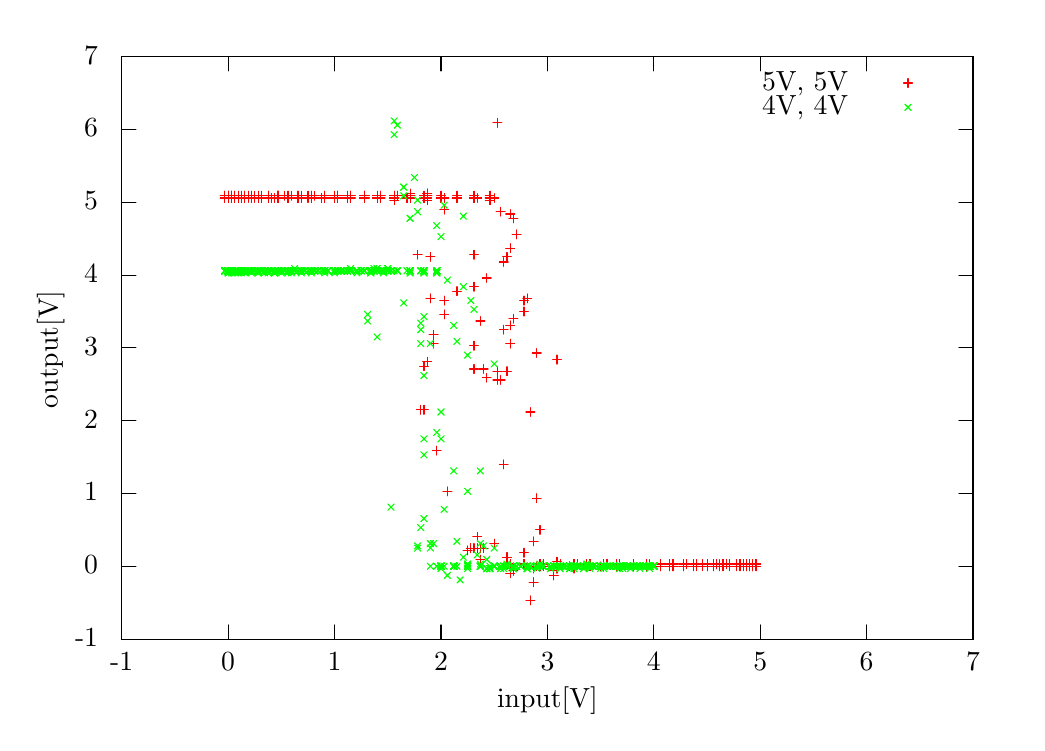
\begin{tikzpicture}[gnuplot]
%% generated with GNUPLOT 4.6p4 (Lua 5.1; terminal rev. 99, script rev. 100)
%% 2016年07月31日 03時48分02秒
\path (0.000,0.000) rectangle (12.500,8.750);
\gpcolor{color=gp lt color border}
\gpsetlinetype{gp lt border}
\gpsetlinewidth{1.00}
\draw[gp path] (1.136,0.985)--(1.316,0.985);
\draw[gp path] (11.947,0.985)--(11.767,0.985);
\node[gp node right] at (0.952,0.985) {-1};
\draw[gp path] (1.136,1.910)--(1.316,1.910);
\draw[gp path] (11.947,1.910)--(11.767,1.910);
\node[gp node right] at (0.952,1.910) { 0};
\draw[gp path] (1.136,2.834)--(1.316,2.834);
\draw[gp path] (11.947,2.834)--(11.767,2.834);
\node[gp node right] at (0.952,2.834) { 1};
\draw[gp path] (1.136,3.759)--(1.316,3.759);
\draw[gp path] (11.947,3.759)--(11.767,3.759);
\node[gp node right] at (0.952,3.759) { 2};
\draw[gp path] (1.136,4.683)--(1.316,4.683);
\draw[gp path] (11.947,4.683)--(11.767,4.683);
\node[gp node right] at (0.952,4.683) { 3};
\draw[gp path] (1.136,5.608)--(1.316,5.608);
\draw[gp path] (11.947,5.608)--(11.767,5.608);
\node[gp node right] at (0.952,5.608) { 4};
\draw[gp path] (1.136,6.532)--(1.316,6.532);
\draw[gp path] (11.947,6.532)--(11.767,6.532);
\node[gp node right] at (0.952,6.532) { 5};
\draw[gp path] (1.136,7.457)--(1.316,7.457);
\draw[gp path] (11.947,7.457)--(11.767,7.457);
\node[gp node right] at (0.952,7.457) { 6};
\draw[gp path] (1.136,8.381)--(1.316,8.381);
\draw[gp path] (11.947,8.381)--(11.767,8.381);
\node[gp node right] at (0.952,8.381) { 7};
\draw[gp path] (1.136,0.985)--(1.136,1.165);
\draw[gp path] (1.136,8.381)--(1.136,8.201);
\node[gp node center] at (1.136,0.677) {-1};
\draw[gp path] (2.487,0.985)--(2.487,1.165);
\draw[gp path] (2.487,8.381)--(2.487,8.201);
\node[gp node center] at (2.487,0.677) { 0};
\draw[gp path] (3.839,0.985)--(3.839,1.165);
\draw[gp path] (3.839,8.381)--(3.839,8.201);
\node[gp node center] at (3.839,0.677) { 1};
\draw[gp path] (5.190,0.985)--(5.190,1.165);
\draw[gp path] (5.190,8.381)--(5.190,8.201);
\node[gp node center] at (5.190,0.677) { 2};
\draw[gp path] (6.542,0.985)--(6.542,1.165);
\draw[gp path] (6.542,8.381)--(6.542,8.201);
\node[gp node center] at (6.542,0.677) { 3};
\draw[gp path] (7.893,0.985)--(7.893,1.165);
\draw[gp path] (7.893,8.381)--(7.893,8.201);
\node[gp node center] at (7.893,0.677) { 4};
\draw[gp path] (9.244,0.985)--(9.244,1.165);
\draw[gp path] (9.244,8.381)--(9.244,8.201);
\node[gp node center] at (9.244,0.677) { 5};
\draw[gp path] (10.596,0.985)--(10.596,1.165);
\draw[gp path] (10.596,8.381)--(10.596,8.201);
\node[gp node center] at (10.596,0.677) { 6};
\draw[gp path] (11.947,0.985)--(11.947,1.165);
\draw[gp path] (11.947,8.381)--(11.947,8.201);
\node[gp node center] at (11.947,0.677) { 7};
\draw[gp path] (1.136,8.381)--(1.136,0.985)--(11.947,0.985)--(11.947,8.381)--cycle;
\node[gp node center,rotate=-270] at (0.246,4.683) {output[V]};
\node[gp node center] at (6.541,0.215) {input[V]};
\node[gp node right] at (10.479,8.047) {5V, 5V};
\gpcolor{color=gp lt color 0}
\gpsetpointsize{4.00}
\gppoint{gp mark 1}{(2.994,6.615)}
\gppoint{gp mark 1}{(3.120,6.587)}
\gppoint{gp mark 1}{(3.247,6.587)}
\gppoint{gp mark 1}{(3.374,6.587)}
\gppoint{gp mark 1}{(3.543,6.587)}
\gppoint{gp mark 1}{(3.670,6.587)}
\gppoint{gp mark 1}{(3.879,6.587)}
\gppoint{gp mark 1}{(4.041,6.587)}
\gppoint{gp mark 1}{(4.217,6.587)}
\gppoint{gp mark 1}{(4.420,6.587)}
\gppoint{gp mark 1}{(4.596,6.587)}
\gppoint{gp mark 1}{(4.798,6.587)}
\gppoint{gp mark 1}{(5.014,6.587)}
\gppoint{gp mark 1}{(5.190,6.587)}
\gppoint{gp mark 1}{(5.393,6.587)}
\gppoint{gp mark 1}{(5.609,6.587)}
\gppoint{gp mark 1}{(5.812,6.560)}
\gppoint{gp mark 1}{(6.028,2.025)}
\gppoint{gp mark 1}{(6.109,5.053)}
\gppoint{gp mark 1}{(5.609,5.866)}
\gppoint{gp mark 1}{(6.663,1.910)}
\gppoint{gp mark 1}{(6.879,1.910)}
\gppoint{gp mark 1}{(7.042,1.910)}
\gppoint{gp mark 1}{(7.258,1.910)}
\gppoint{gp mark 1}{(7.460,1.910)}
\gppoint{gp mark 1}{(7.636,1.910)}
\gppoint{gp mark 1}{(7.798,1.938)}
\gppoint{gp mark 1}{(7.974,1.910)}
\gppoint{gp mark 1}{(8.136,1.938)}
\gppoint{gp mark 1}{(8.271,1.938)}
\gppoint{gp mark 1}{(8.433,1.910)}
\gppoint{gp mark 1}{(8.569,1.910)}
\gppoint{gp mark 1}{(8.650,1.938)}
\gppoint{gp mark 1}{(8.771,1.938)}
\gppoint{gp mark 1}{(8.852,1.938)}
\gppoint{gp mark 1}{(8.947,1.938)}
\gppoint{gp mark 1}{(8.987,1.938)}
\gppoint{gp mark 1}{(9.028,1.938)}
\gppoint{gp mark 1}{(9.109,1.910)}
\gppoint{gp mark 1}{(9.150,1.938)}
\gppoint{gp mark 1}{(9.150,1.938)}
\gppoint{gp mark 1}{(9.150,1.938)}
\gppoint{gp mark 1}{(9.190,1.938)}
\gppoint{gp mark 1}{(9.150,1.938)}
\gppoint{gp mark 1}{(9.109,1.938)}
\gppoint{gp mark 1}{(9.069,1.938)}
\gppoint{gp mark 1}{(8.987,1.938)}
\gppoint{gp mark 1}{(8.947,1.938)}
\gppoint{gp mark 1}{(8.852,1.938)}
\gppoint{gp mark 1}{(8.771,1.938)}
\gppoint{gp mark 1}{(8.690,1.938)}
\gppoint{gp mark 1}{(8.569,1.938)}
\gppoint{gp mark 1}{(8.433,1.938)}
\gppoint{gp mark 1}{(8.271,1.938)}
\gppoint{gp mark 1}{(8.136,1.938)}
\gppoint{gp mark 1}{(7.974,1.938)}
\gppoint{gp mark 1}{(7.798,1.938)}
\gppoint{gp mark 1}{(7.636,1.938)}
\gppoint{gp mark 1}{(7.460,1.938)}
\gppoint{gp mark 1}{(7.258,1.938)}
\gppoint{gp mark 1}{(7.082,1.938)}
\gppoint{gp mark 1}{(6.920,1.938)}
\gppoint{gp mark 1}{(6.663,1.938)}
\gppoint{gp mark 1}{(6.447,1.938)}
\gppoint{gp mark 1}{(6.244,1.938)}
\gppoint{gp mark 1}{(6.028,1.938)}
\gppoint{gp mark 1}{(5.055,5.312)}
\gppoint{gp mark 1}{(6.109,6.329)}
\gppoint{gp mark 1}{(5.569,2.141)}
\gppoint{gp mark 1}{(4.974,4.452)}
\gppoint{gp mark 1}{(5.014,6.643)}
\gppoint{gp mark 1}{(4.798,6.615)}
\gppoint{gp mark 1}{(4.596,6.615)}
\gppoint{gp mark 1}{(4.379,6.615)}
\gppoint{gp mark 1}{(4.217,6.615)}
\gppoint{gp mark 1}{(4.041,6.587)}
\gppoint{gp mark 1}{(3.879,6.615)}
\gppoint{gp mark 1}{(3.712,6.615)}
\gppoint{gp mark 1}{(3.543,6.615)}
\gppoint{gp mark 1}{(3.374,6.587)}
\gppoint{gp mark 1}{(3.247,6.587)}
\gppoint{gp mark 1}{(3.120,6.615)}
\gppoint{gp mark 1}{(2.994,6.587)}
\gppoint{gp mark 1}{(2.909,6.587)}
\gppoint{gp mark 1}{(2.782,6.587)}
\gppoint{gp mark 1}{(2.740,6.615)}
\gppoint{gp mark 1}{(2.614,6.615)}
\gppoint{gp mark 1}{(2.572,6.587)}
\gppoint{gp mark 1}{(2.530,6.587)}
\gppoint{gp mark 1}{(2.487,6.587)}
\gppoint{gp mark 1}{(2.487,6.587)}
\gppoint{gp mark 1}{(2.487,6.587)}
\gppoint{gp mark 1}{(2.445,6.587)}
\gppoint{gp mark 1}{(2.487,6.587)}
\gppoint{gp mark 1}{(2.530,6.587)}
\gppoint{gp mark 1}{(2.572,6.615)}
\gppoint{gp mark 1}{(2.656,6.587)}
\gppoint{gp mark 1}{(2.698,6.587)}
\gppoint{gp mark 1}{(2.825,6.587)}
\gppoint{gp mark 1}{(2.867,6.587)}
\gppoint{gp mark 1}{(2.994,6.587)}
\gppoint{gp mark 1}{(3.120,6.587)}
\gppoint{gp mark 1}{(3.247,6.587)}
\gppoint{gp mark 1}{(3.374,6.587)}
\gppoint{gp mark 1}{(3.543,6.587)}
\gppoint{gp mark 1}{(3.670,6.587)}
\gppoint{gp mark 1}{(3.839,6.587)}
\gppoint{gp mark 1}{(4.001,6.587)}
\gppoint{gp mark 1}{(4.217,6.587)}
\gppoint{gp mark 1}{(4.379,6.587)}
\gppoint{gp mark 1}{(4.596,6.587)}
\gppoint{gp mark 1}{(4.798,6.587)}
\gppoint{gp mark 1}{(4.974,6.587)}
\gppoint{gp mark 1}{(5.190,6.587)}
\gppoint{gp mark 1}{(5.393,6.587)}
\gppoint{gp mark 1}{(5.650,6.587)}
\gppoint{gp mark 1}{(5.812,6.587)}
\gppoint{gp mark 1}{(5.906,4.276)}
\gppoint{gp mark 1}{(6.244,2.082)}
\gppoint{gp mark 1}{(6.366,1.708)}
\gppoint{gp mark 1}{(6.663,1.881)}
\gppoint{gp mark 1}{(6.825,1.910)}
\gppoint{gp mark 1}{(7.042,1.938)}
\gppoint{gp mark 1}{(7.258,1.910)}
\gppoint{gp mark 1}{(7.420,1.910)}
\gppoint{gp mark 1}{(7.636,1.910)}
\gppoint{gp mark 1}{(7.798,1.910)}
\gppoint{gp mark 1}{(7.974,1.910)}
\gppoint{gp mark 1}{(8.096,1.910)}
\gppoint{gp mark 1}{(8.271,1.938)}
\gppoint{gp mark 1}{(8.433,1.938)}
\gppoint{gp mark 1}{(8.515,1.910)}
\gppoint{gp mark 1}{(8.650,1.910)}
\gppoint{gp mark 1}{(8.731,1.938)}
\gppoint{gp mark 1}{(8.852,1.938)}
\gppoint{gp mark 1}{(8.947,1.910)}
\gppoint{gp mark 1}{(8.987,1.910)}
\gppoint{gp mark 1}{(9.069,1.910)}
\gppoint{gp mark 1}{(9.109,1.910)}
\gppoint{gp mark 1}{(9.150,1.938)}
\gppoint{gp mark 1}{(9.150,1.938)}
\gppoint{gp mark 1}{(9.190,1.938)}
\gppoint{gp mark 1}{(9.150,1.938)}
\gppoint{gp mark 1}{(9.150,1.910)}
\gppoint{gp mark 1}{(9.109,1.938)}
\gppoint{gp mark 1}{(9.069,1.938)}
\gppoint{gp mark 1}{(9.028,1.938)}
\gppoint{gp mark 1}{(8.947,1.938)}
\gppoint{gp mark 1}{(8.852,1.938)}
\gppoint{gp mark 1}{(8.771,1.938)}
\gppoint{gp mark 1}{(8.690,1.938)}
\gppoint{gp mark 1}{(8.569,1.938)}
\gppoint{gp mark 1}{(8.433,1.938)}
\gppoint{gp mark 1}{(8.271,1.938)}
\gppoint{gp mark 1}{(8.136,1.938)}
\gppoint{gp mark 1}{(7.974,1.938)}
\gppoint{gp mark 1}{(7.798,1.938)}
\gppoint{gp mark 1}{(7.636,1.938)}
\gppoint{gp mark 1}{(7.460,1.938)}
\gppoint{gp mark 1}{(7.298,1.938)}
\gppoint{gp mark 1}{(7.082,1.938)}
\gppoint{gp mark 1}{(6.920,1.938)}
\gppoint{gp mark 1}{(6.663,1.938)}
\gppoint{gp mark 1}{(6.447,1.910)}
\gppoint{gp mark 1}{(6.244,1.938)}
\gppoint{gp mark 1}{(6.028,1.938)}
\gppoint{gp mark 1}{(5.731,4.415)}
\gppoint{gp mark 1}{(5.987,5.774)}
\gppoint{gp mark 1}{(5.690,2.141)}
\gppoint{gp mark 1}{(5.096,4.738)}
\gppoint{gp mark 1}{(5.014,6.615)}
\gppoint{gp mark 1}{(4.798,6.615)}
\gppoint{gp mark 1}{(4.636,6.615)}
\gppoint{gp mark 1}{(4.420,6.615)}
\gppoint{gp mark 1}{(4.217,6.615)}
\gppoint{gp mark 1}{(4.041,6.615)}
\gppoint{gp mark 1}{(3.879,6.615)}
\gppoint{gp mark 1}{(3.712,6.587)}
\gppoint{gp mark 1}{(3.543,6.587)}
\gppoint{gp mark 1}{(3.374,6.587)}
\gppoint{gp mark 1}{(3.247,6.587)}
\gppoint{gp mark 1}{(3.120,6.587)}
\gppoint{gp mark 1}{(3.036,6.587)}
\gppoint{gp mark 1}{(2.909,6.587)}
\gppoint{gp mark 1}{(2.782,6.615)}
\gppoint{gp mark 1}{(2.740,6.587)}
\gppoint{gp mark 1}{(2.656,6.615)}
\gppoint{gp mark 1}{(2.572,6.587)}
\gppoint{gp mark 1}{(2.530,6.587)}
\gppoint{gp mark 1}{(2.487,6.615)}
\gppoint{gp mark 1}{(2.445,6.615)}
\gppoint{gp mark 1}{(2.445,6.615)}
\gppoint{gp mark 1}{(2.445,6.587)}
\gppoint{gp mark 1}{(2.530,6.587)}
\gppoint{gp mark 1}{(2.530,6.615)}
\gppoint{gp mark 1}{(2.572,6.615)}
\gppoint{gp mark 1}{(2.656,6.587)}
\gppoint{gp mark 1}{(2.698,6.587)}
\gppoint{gp mark 1}{(2.782,6.587)}
\gppoint{gp mark 1}{(2.867,6.587)}
\gppoint{gp mark 1}{(2.994,6.587)}
\gppoint{gp mark 1}{(3.120,6.615)}
\gppoint{gp mark 1}{(3.205,6.615)}
\gppoint{gp mark 1}{(3.374,6.587)}
\gppoint{gp mark 1}{(3.501,6.615)}
\gppoint{gp mark 1}{(3.712,6.587)}
\gppoint{gp mark 1}{(3.879,6.615)}
\gppoint{gp mark 1}{(4.001,6.615)}
\gppoint{gp mark 1}{(4.217,6.587)}
\gppoint{gp mark 1}{(4.379,6.587)}
\gppoint{gp mark 1}{(4.596,6.587)}
\gppoint{gp mark 1}{(4.758,6.587)}
\gppoint{gp mark 1}{(4.974,6.587)}
\gppoint{gp mark 1}{(5.190,6.587)}
\gppoint{gp mark 1}{(5.393,6.587)}
\gppoint{gp mark 1}{(5.609,6.587)}
\gppoint{gp mark 1}{(5.812,6.587)}
\gppoint{gp mark 1}{(6.028,4.387)}
\gppoint{gp mark 1}{(6.325,3.869)}
\gppoint{gp mark 1}{(5.987,3.204)}
\gppoint{gp mark 1}{(6.663,1.910)}
\gppoint{gp mark 1}{(6.879,1.910)}
\gppoint{gp mark 1}{(7.042,1.910)}
\gppoint{gp mark 1}{(7.258,1.938)}
\gppoint{gp mark 1}{(7.420,1.938)}
\gppoint{gp mark 1}{(7.636,1.910)}
\gppoint{gp mark 1}{(7.798,1.910)}
\gppoint{gp mark 1}{(7.974,1.910)}
\gppoint{gp mark 1}{(8.096,1.910)}
\gppoint{gp mark 1}{(8.312,1.938)}
\gppoint{gp mark 1}{(8.433,1.910)}
\gppoint{gp mark 1}{(8.569,1.938)}
\gppoint{gp mark 1}{(8.650,1.938)}
\gppoint{gp mark 1}{(8.771,1.938)}
\gppoint{gp mark 1}{(8.852,1.938)}
\gppoint{gp mark 1}{(8.947,1.910)}
\gppoint{gp mark 1}{(9.028,1.938)}
\gppoint{gp mark 1}{(9.069,1.938)}
\gppoint{gp mark 1}{(9.109,1.938)}
\gppoint{gp mark 1}{(9.150,1.938)}
\gppoint{gp mark 1}{(9.150,1.938)}
\gppoint{gp mark 1}{(9.190,1.910)}
\gppoint{gp mark 1}{(9.150,1.938)}
\gppoint{gp mark 1}{(9.150,1.938)}
\gppoint{gp mark 1}{(9.109,1.938)}
\gppoint{gp mark 1}{(9.069,1.938)}
\gppoint{gp mark 1}{(9.028,1.938)}
\gppoint{gp mark 1}{(8.947,1.938)}
\gppoint{gp mark 1}{(8.852,1.910)}
\gppoint{gp mark 1}{(8.771,1.938)}
\gppoint{gp mark 1}{(8.650,1.910)}
\gppoint{gp mark 1}{(8.569,1.938)}
\gppoint{gp mark 1}{(8.433,1.938)}
\gppoint{gp mark 1}{(8.312,1.938)}
\gppoint{gp mark 1}{(8.136,1.938)}
\gppoint{gp mark 1}{(7.974,1.938)}
\gppoint{gp mark 1}{(7.839,1.938)}
\gppoint{gp mark 1}{(7.636,1.938)}
\gppoint{gp mark 1}{(7.460,1.938)}
\gppoint{gp mark 1}{(7.258,1.938)}
\gppoint{gp mark 1}{(7.082,1.938)}
\gppoint{gp mark 1}{(6.879,1.938)}
\gppoint{gp mark 1}{(6.663,1.938)}
\gppoint{gp mark 1}{(6.447,1.938)}
\gppoint{gp mark 1}{(6.244,1.938)}
\gppoint{gp mark 1}{(6.069,1.938)}
\gppoint{gp mark 1}{(6.285,5.312)}
\gppoint{gp mark 1}{(5.690,1.996)}
\gppoint{gp mark 1}{(5.271,2.862)}
\gppoint{gp mark 1}{(5.055,5.839)}
\gppoint{gp mark 1}{(5.014,6.560)}
\gppoint{gp mark 1}{(4.798,6.615)}
\gppoint{gp mark 1}{(4.596,6.615)}
\gppoint{gp mark 1}{(4.420,6.615)}
\gppoint{gp mark 1}{(4.217,6.587)}
\gppoint{gp mark 1}{(4.041,6.615)}
\gppoint{gp mark 1}{(3.879,6.615)}
\gppoint{gp mark 1}{(3.712,6.615)}
\gppoint{gp mark 1}{(3.585,6.615)}
\gppoint{gp mark 1}{(3.416,6.615)}
\gppoint{gp mark 1}{(3.247,6.615)}
\gppoint{gp mark 1}{(3.120,6.615)}
\gppoint{gp mark 1}{(2.994,6.615)}
\gppoint{gp mark 1}{(2.909,6.615)}
\gppoint{gp mark 1}{(2.825,6.615)}
\gppoint{gp mark 1}{(2.698,6.615)}
\gppoint{gp mark 1}{(2.614,6.615)}
\gppoint{gp mark 1}{(2.572,6.615)}
\gppoint{gp mark 1}{(2.530,6.615)}
\gppoint{gp mark 1}{(2.530,6.615)}
\gppoint{gp mark 1}{(2.445,6.587)}
\gppoint{gp mark 1}{(2.487,6.615)}
\gppoint{gp mark 1}{(2.487,6.587)}
\gppoint{gp mark 1}{(2.530,6.587)}
\gppoint{gp mark 1}{(2.530,6.587)}
\gppoint{gp mark 1}{(2.572,6.587)}
\gppoint{gp mark 1}{(2.656,6.587)}
\gppoint{gp mark 1}{(2.698,6.587)}
\gppoint{gp mark 1}{(2.782,6.587)}
\gppoint{gp mark 1}{(2.867,6.615)}
\gppoint{gp mark 1}{(2.994,6.587)}
\gppoint{gp mark 1}{(3.078,6.587)}
\gppoint{gp mark 1}{(3.247,6.587)}
\gppoint{gp mark 1}{(3.374,6.587)}
\gppoint{gp mark 1}{(3.501,6.587)}
\gppoint{gp mark 1}{(3.670,6.587)}
\gppoint{gp mark 1}{(3.839,6.615)}
\gppoint{gp mark 1}{(4.001,6.587)}
\gppoint{gp mark 1}{(4.217,6.587)}
\gppoint{gp mark 1}{(4.379,6.587)}
\gppoint{gp mark 1}{(4.596,6.587)}
\gppoint{gp mark 1}{(4.798,6.615)}
\gppoint{gp mark 1}{(4.974,6.587)}
\gppoint{gp mark 1}{(5.190,6.587)}
\gppoint{gp mark 1}{(5.393,6.587)}
\gppoint{gp mark 1}{(5.609,6.615)}
\gppoint{gp mark 1}{(5.812,6.615)}
\gppoint{gp mark 1}{(6.028,5.839)}
\gppoint{gp mark 1}{(6.069,1.823)}
\gppoint{gp mark 1}{(6.623,1.794)}
\gppoint{gp mark 1}{(6.663,1.910)}
\gppoint{gp mark 1}{(6.879,1.910)}
\gppoint{gp mark 1}{(7.042,1.910)}
\gppoint{gp mark 1}{(7.217,1.910)}
\gppoint{gp mark 1}{(7.420,1.910)}
\gppoint{gp mark 1}{(7.636,1.910)}
\gppoint{gp mark 1}{(7.798,1.938)}
\gppoint{gp mark 1}{(7.974,1.938)}
\gppoint{gp mark 1}{(8.096,1.938)}
\gppoint{gp mark 1}{(8.271,1.910)}
\gppoint{gp mark 1}{(8.433,1.938)}
\gppoint{gp mark 1}{(8.569,1.910)}
\gppoint{gp mark 1}{(8.650,1.910)}
\gppoint{gp mark 1}{(8.731,1.910)}
\gppoint{gp mark 1}{(8.852,1.938)}
\gppoint{gp mark 1}{(8.947,1.938)}
\gppoint{gp mark 1}{(8.987,1.910)}
\gppoint{gp mark 1}{(9.069,1.938)}
\gppoint{gp mark 1}{(9.109,1.938)}
\gppoint{gp mark 1}{(9.150,1.938)}
\gppoint{gp mark 1}{(9.150,1.938)}
\gppoint{gp mark 1}{(9.150,1.938)}
\gppoint{gp mark 1}{(9.190,1.938)}
\gppoint{gp mark 1}{(9.150,1.938)}
\gppoint{gp mark 1}{(9.109,1.938)}
\gppoint{gp mark 1}{(9.069,1.938)}
\gppoint{gp mark 1}{(9.028,1.938)}
\gppoint{gp mark 1}{(8.947,1.938)}
\gppoint{gp mark 1}{(8.852,1.938)}
\gppoint{gp mark 1}{(8.771,1.938)}
\gppoint{gp mark 1}{(8.650,1.938)}
\gppoint{gp mark 1}{(8.569,1.938)}
\gppoint{gp mark 1}{(8.433,1.938)}
\gppoint{gp mark 1}{(8.271,1.938)}
\gppoint{gp mark 1}{(8.136,1.938)}
\gppoint{gp mark 1}{(7.974,1.938)}
\gppoint{gp mark 1}{(7.798,1.938)}
\gppoint{gp mark 1}{(7.636,1.938)}
\gppoint{gp mark 1}{(7.460,1.938)}
\gppoint{gp mark 1}{(7.258,1.938)}
\gppoint{gp mark 1}{(7.042,1.938)}
\gppoint{gp mark 1}{(6.879,1.938)}
\gppoint{gp mark 1}{(6.704,1.938)}
\gppoint{gp mark 1}{(6.447,1.938)}
\gppoint{gp mark 1}{(6.244,1.938)}
\gppoint{gp mark 1}{(6.069,1.938)}
\gppoint{gp mark 1}{(5.771,4.304)}
\gppoint{gp mark 1}{(6.069,6.384)}
\gppoint{gp mark 1}{(5.569,2.141)}
\gppoint{gp mark 1}{(5.014,4.507)}
\gppoint{gp mark 1}{(5.014,6.615)}
\gppoint{gp mark 1}{(4.798,6.615)}
\gppoint{gp mark 1}{(4.596,6.615)}
\gppoint{gp mark 1}{(4.420,6.615)}
\gppoint{gp mark 1}{(4.217,6.587)}
\gppoint{gp mark 1}{(4.041,6.615)}
\gppoint{gp mark 1}{(3.879,6.615)}
\gppoint{gp mark 1}{(3.712,6.587)}
\gppoint{gp mark 1}{(3.543,6.587)}
\gppoint{gp mark 1}{(3.374,6.615)}
\gppoint{gp mark 1}{(3.247,6.587)}
\gppoint{gp mark 1}{(3.120,6.615)}
\gppoint{gp mark 1}{(2.994,6.587)}
\gppoint{gp mark 1}{(2.909,6.615)}
\gppoint{gp mark 1}{(2.782,6.615)}
\gppoint{gp mark 1}{(2.698,6.587)}
\gppoint{gp mark 1}{(2.656,6.615)}
\gppoint{gp mark 1}{(2.614,6.615)}
\gppoint{gp mark 1}{(2.530,6.587)}
\gppoint{gp mark 1}{(2.487,6.587)}
\gppoint{gp mark 1}{(2.445,6.615)}
\gppoint{gp mark 1}{(2.487,6.615)}
\gppoint{gp mark 1}{(2.487,6.587)}
\gppoint{gp mark 1}{(2.487,6.615)}
\gppoint{gp mark 1}{(2.530,6.587)}
\gppoint{gp mark 1}{(2.572,6.587)}
\gppoint{gp mark 1}{(2.614,6.587)}
\gppoint{gp mark 1}{(2.698,6.587)}
\gppoint{gp mark 1}{(2.782,6.587)}
\gppoint{gp mark 1}{(2.867,6.587)}
\gppoint{gp mark 1}{(2.994,6.587)}
\gppoint{gp mark 1}{(3.120,6.587)}
\gppoint{gp mark 1}{(3.247,6.587)}
\gppoint{gp mark 1}{(3.374,6.615)}
\gppoint{gp mark 1}{(3.543,6.615)}
\gppoint{gp mark 1}{(3.670,6.587)}
\gppoint{gp mark 1}{(3.839,6.615)}
\gppoint{gp mark 1}{(4.001,6.587)}
\gppoint{gp mark 1}{(4.217,6.587)}
\gppoint{gp mark 1}{(4.379,6.587)}
\gppoint{gp mark 1}{(4.596,6.587)}
\gppoint{gp mark 1}{(4.758,6.587)}
\gppoint{gp mark 1}{(4.974,6.587)}
\gppoint{gp mark 1}{(5.190,6.615)}
\gppoint{gp mark 1}{(5.393,6.587)}
\gppoint{gp mark 1}{(5.609,6.587)}
\gppoint{gp mark 1}{(5.812,6.560)}
\gppoint{gp mark 1}{(6.244,5.284)}
\gppoint{gp mark 1}{(6.406,4.618)}
\gppoint{gp mark 1}{(5.609,4.415)}
\gppoint{gp mark 1}{(6.663,1.910)}
\gppoint{gp mark 1}{(6.879,1.910)}
\gppoint{gp mark 1}{(7.042,1.910)}
\gppoint{gp mark 1}{(7.258,1.910)}
\gppoint{gp mark 1}{(7.420,1.938)}
\gppoint{gp mark 1}{(7.636,1.938)}
\gppoint{gp mark 1}{(7.798,1.910)}
\gppoint{gp mark 1}{(7.974,1.938)}
\gppoint{gp mark 1}{(8.096,1.910)}
\gppoint{gp mark 1}{(8.271,1.938)}
\gppoint{gp mark 1}{(8.433,1.938)}
\gppoint{gp mark 1}{(8.515,1.938)}
\gppoint{gp mark 1}{(8.650,1.910)}
\gppoint{gp mark 1}{(8.771,1.938)}
\gppoint{gp mark 1}{(8.852,1.938)}
\gppoint{gp mark 1}{(8.947,1.938)}
\gppoint{gp mark 1}{(8.987,1.938)}
\gppoint{gp mark 1}{(9.109,1.938)}
\gppoint{gp mark 1}{(9.109,1.938)}
\gppoint{gp mark 1}{(9.150,1.938)}
\gppoint{gp mark 1}{(9.190,1.938)}
\gppoint{gp mark 1}{(9.190,1.938)}
\gppoint{gp mark 1}{(9.190,1.938)}
\gppoint{gp mark 1}{(9.150,1.938)}
\gppoint{gp mark 1}{(9.109,1.938)}
\gppoint{gp mark 1}{(9.069,1.938)}
\gppoint{gp mark 1}{(9.028,1.938)}
\gppoint{gp mark 1}{(8.947,1.938)}
\gppoint{gp mark 1}{(8.852,1.938)}
\gppoint{gp mark 1}{(8.771,1.938)}
\gppoint{gp mark 1}{(8.690,1.938)}
\gppoint{gp mark 1}{(8.569,1.910)}
\gppoint{gp mark 1}{(8.433,1.938)}
\gppoint{gp mark 1}{(8.271,1.938)}
\gppoint{gp mark 1}{(8.136,1.910)}
\gppoint{gp mark 1}{(7.974,1.938)}
\gppoint{gp mark 1}{(7.798,1.938)}
\gppoint{gp mark 1}{(7.636,1.938)}
\gppoint{gp mark 1}{(7.460,1.938)}
\gppoint{gp mark 1}{(7.298,1.938)}
\gppoint{gp mark 1}{(7.042,1.938)}
\gppoint{gp mark 1}{(6.879,1.938)}
\gppoint{gp mark 1}{(6.704,1.938)}
\gppoint{gp mark 1}{(6.487,1.938)}
\gppoint{gp mark 1}{(6.244,1.938)}
\gppoint{gp mark 1}{(6.069,1.938)}
\gppoint{gp mark 1}{(5.136,3.379)}
\gppoint{gp mark 1}{(6.069,5.950)}
\gppoint{gp mark 1}{(5.609,2.141)}
\gppoint{gp mark 1}{(4.974,3.897)}
\gppoint{gp mark 1}{(5.014,6.643)}
\gppoint{gp mark 1}{(4.798,6.615)}
\gppoint{gp mark 1}{(4.636,6.615)}
\gppoint{gp mark 1}{(4.379,6.615)}
\gppoint{gp mark 1}{(4.217,6.615)}
\gppoint{gp mark 1}{(4.041,6.615)}
\gppoint{gp mark 1}{(3.879,6.615)}
\gppoint{gp mark 1}{(3.712,6.587)}
\gppoint{gp mark 1}{(3.543,6.615)}
\gppoint{gp mark 1}{(3.416,6.615)}
\gppoint{gp mark 1}{(3.247,6.587)}
\gppoint{gp mark 1}{(3.120,6.587)}
\gppoint{gp mark 1}{(2.994,6.587)}
\gppoint{gp mark 1}{(2.909,6.587)}
\gppoint{gp mark 1}{(2.782,6.615)}
\gppoint{gp mark 1}{(2.740,6.615)}
\gppoint{gp mark 1}{(2.614,6.587)}
\gppoint{gp mark 1}{(2.572,6.587)}
\gppoint{gp mark 1}{(2.530,6.615)}
\gppoint{gp mark 1}{(2.487,6.587)}
\gppoint{gp mark 1}{(2.487,6.587)}
\gppoint{gp mark 1}{(2.487,6.615)}
\gppoint{gp mark 1}{(2.487,6.587)}
\gppoint{gp mark 1}{(2.487,6.587)}
\gppoint{gp mark 1}{(2.530,6.587)}
\gppoint{gp mark 1}{(2.572,6.587)}
\gppoint{gp mark 1}{(2.614,6.587)}
\gppoint{gp mark 1}{(2.698,6.615)}
\gppoint{gp mark 1}{(2.782,6.587)}
\gppoint{gp mark 1}{(2.867,6.587)}
\gppoint{gp mark 1}{(2.994,6.587)}
\gppoint{gp mark 1}{(3.120,6.587)}
\gppoint{gp mark 1}{(3.247,6.587)}
\gppoint{gp mark 1}{(3.374,6.587)}
\gppoint{gp mark 1}{(3.543,6.587)}
\gppoint{gp mark 1}{(3.670,6.587)}
\gppoint{gp mark 1}{(3.839,6.587)}
\gppoint{gp mark 1}{(4.001,6.587)}
\gppoint{gp mark 1}{(4.217,6.587)}
\gppoint{gp mark 1}{(4.379,6.587)}
\gppoint{gp mark 1}{(4.596,6.587)}
\gppoint{gp mark 1}{(4.798,6.587)}
\gppoint{gp mark 1}{(4.974,6.587)}
\gppoint{gp mark 1}{(5.190,6.587)}
\gppoint{gp mark 1}{(5.393,6.587)}
\gppoint{gp mark 1}{(5.609,6.587)}
\gppoint{gp mark 1}{(5.812,6.587)}
\gppoint{gp mark 1}{(5.609,4.711)}
\gppoint{gp mark 1}{(6.406,2.776)}
\gppoint{gp mark 1}{(6.325,1.477)}
\gppoint{gp mark 1}{(6.663,1.910)}
\gppoint{gp mark 1}{(6.879,1.910)}
\gppoint{gp mark 1}{(7.042,1.910)}
\gppoint{gp mark 1}{(7.258,1.910)}
\gppoint{gp mark 1}{(7.460,1.910)}
\gppoint{gp mark 1}{(7.636,1.938)}
\gppoint{gp mark 1}{(7.798,1.910)}
\gppoint{gp mark 1}{(7.974,1.938)}
\gppoint{gp mark 1}{(8.136,1.910)}
\gppoint{gp mark 1}{(8.271,1.938)}
\gppoint{gp mark 1}{(8.393,1.938)}
\gppoint{gp mark 1}{(8.569,1.938)}
\gppoint{gp mark 1}{(8.650,1.910)}
\gppoint{gp mark 1}{(8.731,1.910)}
\gppoint{gp mark 1}{(8.852,1.938)}
\gppoint{gp mark 1}{(8.947,1.910)}
\gppoint{gp mark 1}{(9.028,1.938)}
\gppoint{gp mark 1}{(9.069,1.938)}
\gppoint{gp mark 1}{(9.109,1.938)}
\gppoint{gp mark 1}{(9.150,1.910)}
\gppoint{gp mark 1}{(9.150,1.910)}
\gppoint{gp mark 1}{(9.150,1.938)}
\gppoint{gp mark 1}{(9.190,1.938)}
\gppoint{gp mark 1}{(9.109,1.910)}
\gppoint{gp mark 1}{(9.109,1.910)}
\gppoint{gp mark 1}{(9.069,1.938)}
\gppoint{gp mark 1}{(9.028,1.938)}
\gppoint{gp mark 1}{(8.947,1.938)}
\gppoint{gp mark 1}{(8.852,1.938)}
\gppoint{gp mark 1}{(8.771,1.938)}
\gppoint{gp mark 1}{(8.650,1.938)}
\gppoint{gp mark 1}{(8.569,1.910)}
\gppoint{gp mark 1}{(8.433,1.938)}
\gppoint{gp mark 1}{(8.271,1.938)}
\gppoint{gp mark 1}{(8.136,1.938)}
\gppoint{gp mark 1}{(7.974,1.938)}
\gppoint{gp mark 1}{(7.798,1.938)}
\gppoint{gp mark 1}{(7.636,1.938)}
\gppoint{gp mark 1}{(7.460,1.938)}
\gppoint{gp mark 1}{(7.258,1.938)}
\gppoint{gp mark 1}{(7.082,1.938)}
\gppoint{gp mark 1}{(6.920,1.938)}
\gppoint{gp mark 1}{(6.663,1.938)}
\gppoint{gp mark 1}{(6.447,1.938)}
\gppoint{gp mark 1}{(6.244,1.938)}
\gppoint{gp mark 1}{(6.028,1.938)}
\gppoint{gp mark 1}{(6.069,4.970)}
\gppoint{gp mark 1}{(5.771,5.571)}
\gppoint{gp mark 1}{(5.650,2.141)}
\gppoint{gp mark 1}{(5.096,4.849)}
\gppoint{gp mark 1}{(5.014,6.615)}
\gppoint{gp mark 1}{(4.798,6.643)}
\gppoint{gp mark 1}{(4.596,6.615)}
\gppoint{gp mark 1}{(4.379,6.615)}
\gppoint{gp mark 1}{(4.217,6.615)}
\gppoint{gp mark 1}{(4.041,6.615)}
\gppoint{gp mark 1}{(3.839,6.615)}
\gppoint{gp mark 1}{(3.712,6.615)}
\gppoint{gp mark 1}{(3.543,6.615)}
\gppoint{gp mark 1}{(3.374,6.615)}
\gppoint{gp mark 1}{(3.247,6.615)}
\gppoint{gp mark 1}{(3.120,6.615)}
\gppoint{gp mark 1}{(2.994,6.587)}
\gppoint{gp mark 1}{(2.909,6.615)}
\gppoint{gp mark 1}{(2.782,6.615)}
\gppoint{gp mark 1}{(2.698,6.587)}
\gppoint{gp mark 1}{(2.614,6.587)}
\gppoint{gp mark 1}{(2.572,6.615)}
\gppoint{gp mark 1}{(2.530,6.615)}
\gppoint{gp mark 1}{(2.487,6.587)}
\gppoint{gp mark 1}{(2.445,6.615)}
\gppoint{gp mark 1}{(2.487,6.587)}
\gppoint{gp mark 1}{(2.487,6.587)}
\gppoint{gp mark 1}{(2.487,6.587)}
\gppoint{gp mark 1}{(2.530,6.615)}
\gppoint{gp mark 1}{(2.572,6.587)}
\gppoint{gp mark 1}{(2.614,6.587)}
\gppoint{gp mark 1}{(2.698,6.615)}
\gppoint{gp mark 1}{(2.782,6.587)}
\gppoint{gp mark 1}{(2.867,6.587)}
\gppoint{gp mark 1}{(2.994,6.615)}
\gppoint{gp mark 1}{(3.120,6.587)}
\gppoint{gp mark 1}{(3.247,6.587)}
\gppoint{gp mark 1}{(3.374,6.587)}
\gppoint{gp mark 1}{(3.543,6.587)}
\gppoint{gp mark 1}{(3.712,6.587)}
\gppoint{gp mark 1}{(3.839,6.587)}
\gppoint{gp mark 1}{(4.041,6.615)}
\gppoint{gp mark 1}{(4.217,6.587)}
\gppoint{gp mark 1}{(4.379,6.587)}
\gppoint{gp mark 1}{(4.596,6.587)}
\gppoint{gp mark 1}{(4.758,6.587)}
\gppoint{gp mark 1}{(4.974,6.587)}
\gppoint{gp mark 1}{(5.231,6.587)}
\gppoint{gp mark 1}{(5.393,6.587)}
\gppoint{gp mark 1}{(5.609,6.587)}
\gppoint{gp mark 1}{(5.812,6.615)}
\gppoint{gp mark 1}{(6.244,5.145)}
\gppoint{gp mark 1}{(6.366,2.227)}
\gppoint{gp mark 1}{(6.447,2.372)}
\gppoint{gp mark 1}{(6.663,1.910)}
\gppoint{gp mark 1}{(6.879,1.881)}
\gppoint{gp mark 1}{(7.042,1.910)}
\gppoint{gp mark 1}{(7.258,1.910)}
\gppoint{gp mark 1}{(7.460,1.938)}
\gppoint{gp mark 1}{(7.636,1.910)}
\gppoint{gp mark 1}{(7.798,1.910)}
\gppoint{gp mark 1}{(7.974,1.910)}
\gppoint{gp mark 1}{(8.096,1.938)}
\gppoint{gp mark 1}{(8.271,1.910)}
\gppoint{gp mark 1}{(8.393,1.910)}
\gppoint{gp mark 1}{(8.569,1.938)}
\gppoint{gp mark 1}{(8.650,1.938)}
\gppoint{gp mark 1}{(8.731,1.910)}
\gppoint{gp mark 1}{(8.812,1.938)}
\gppoint{gp mark 1}{(8.947,1.938)}
\gppoint{gp mark 1}{(9.028,1.938)}
\gppoint{gp mark 1}{(9.069,1.910)}
\gppoint{gp mark 1}{(9.150,1.910)}
\gppoint{gp mark 1}{(9.150,1.910)}
\gppoint{gp mark 1}{(9.190,1.938)}
\gppoint{gp mark 1}{(9.190,1.910)}
\gppoint{gp mark 1}{(9.150,1.938)}
\gppoint{gp mark 1}{(9.150,1.938)}
\gppoint{gp mark 1}{(9.109,1.938)}
\gppoint{gp mark 1}{(9.069,1.910)}
\gppoint{gp mark 1}{(9.028,1.938)}
\gppoint{gp mark 1}{(8.947,1.938)}
\gppoint{gp mark 1}{(8.852,1.938)}
\gppoint{gp mark 1}{(8.771,1.938)}
\gppoint{gp mark 1}{(8.690,1.938)}
\gppoint{gp mark 1}{(8.569,1.938)}
\gppoint{gp mark 1}{(8.433,1.938)}
\gppoint{gp mark 1}{(8.271,1.938)}
\gppoint{gp mark 1}{(8.096,1.938)}
\gppoint{gp mark 1}{(7.974,1.938)}
\gppoint{gp mark 1}{(7.798,1.938)}
\gppoint{gp mark 1}{(7.636,1.910)}
\gppoint{gp mark 1}{(7.460,1.938)}
\gppoint{gp mark 1}{(7.258,1.938)}
\gppoint{gp mark 1}{(7.082,1.910)}
\gppoint{gp mark 1}{(6.879,1.938)}
\gppoint{gp mark 1}{(6.663,1.938)}
\gppoint{gp mark 1}{(6.447,1.938)}
\gppoint{gp mark 1}{(6.244,1.938)}
\gppoint{gp mark 1}{(6.028,1.938)}
\gppoint{gp mark 1}{(5.987,4.914)}
\gppoint{gp mark 1}{(5.947,6.412)}
\gppoint{gp mark 1}{(5.528,2.111)}
\gppoint{gp mark 1}{(4.933,3.897)}
\gppoint{gp mark 1}{(4.974,6.615)}
\gppoint{gp mark 1}{(4.798,6.615)}
\gppoint{gp mark 1}{(4.636,6.615)}
\gppoint{gp mark 1}{(4.420,6.615)}
\gppoint{gp mark 1}{(4.217,6.615)}
\gppoint{gp mark 1}{(4.001,6.615)}
\gppoint{gp mark 1}{(3.839,6.587)}
\gppoint{gp mark 1}{(3.670,6.587)}
\gppoint{gp mark 1}{(3.543,6.615)}
\gppoint{gp mark 1}{(3.374,6.587)}
\gppoint{gp mark 1}{(3.247,6.587)}
\gppoint{gp mark 1}{(3.120,6.615)}
\gppoint{gp mark 1}{(2.994,6.615)}
\gppoint{gp mark 1}{(2.909,6.587)}
\gppoint{gp mark 1}{(2.782,6.587)}
\gppoint{gp mark 1}{(2.740,6.615)}
\gppoint{gp mark 1}{(2.614,6.587)}
\gppoint{gp mark 1}{(2.572,6.587)}
\gppoint{gp mark 1}{(2.530,6.615)}
\gppoint{gp mark 1}{(2.487,6.587)}
\gppoint{gp mark 1}{(2.487,6.587)}
\gppoint{gp mark 1}{(2.487,6.587)}
\gppoint{gp mark 1}{(2.445,6.615)}
\gppoint{gp mark 1}{(2.487,6.587)}
\gppoint{gp mark 1}{(2.530,6.615)}
\gppoint{gp mark 1}{(2.572,6.587)}
\gppoint{gp mark 1}{(2.614,6.587)}
\gppoint{gp mark 1}{(2.698,6.615)}
\gppoint{gp mark 1}{(2.782,6.587)}
\gppoint{gp mark 1}{(2.909,6.587)}
\gppoint{gp mark 1}{(2.994,6.587)}
\gppoint{gp mark 1}{(3.120,6.587)}
\gppoint{gp mark 1}{(3.247,6.587)}
\gppoint{gp mark 1}{(3.374,6.615)}
\gppoint{gp mark 1}{(3.543,6.587)}
\gppoint{gp mark 1}{(3.670,6.587)}
\gppoint{gp mark 1}{(3.839,6.587)}
\gppoint{gp mark 1}{(4.001,6.587)}
\gppoint{gp mark 1}{(4.217,6.615)}
\gppoint{gp mark 1}{(4.379,6.587)}
\gppoint{gp mark 1}{(4.596,6.587)}
\gppoint{gp mark 1}{(4.798,6.587)}
\gppoint{gp mark 1}{(4.974,6.587)}
\gppoint{gp mark 1}{(5.190,6.587)}
\gppoint{gp mark 1}{(5.393,6.615)}
\gppoint{gp mark 1}{(5.609,6.587)}
\gppoint{gp mark 1}{(5.812,6.587)}
\gppoint{gp mark 1}{(5.906,4.387)}
\gppoint{gp mark 1}{(6.663,4.535)}
\gppoint{gp mark 1}{(6.366,1.881)}
\gppoint{gp mark 1}{(6.663,1.910)}
\gppoint{gp mark 1}{(6.879,1.938)}
\gppoint{gp mark 1}{(7.042,1.910)}
\gppoint{gp mark 1}{(7.258,1.910)}
\gppoint{gp mark 1}{(7.420,1.938)}
\gppoint{gp mark 1}{(7.636,1.938)}
\gppoint{gp mark 1}{(7.798,1.910)}
\gppoint{gp mark 1}{(7.974,1.910)}
\gppoint{gp mark 1}{(8.136,1.938)}
\gppoint{gp mark 1}{(8.271,1.910)}
\gppoint{gp mark 1}{(8.433,1.938)}
\gppoint{gp mark 1}{(8.569,1.938)}
\gppoint{gp mark 1}{(8.650,1.938)}
\gppoint{gp mark 1}{(8.771,1.938)}
\gppoint{gp mark 1}{(8.852,1.938)}
\gppoint{gp mark 1}{(8.947,1.938)}
\gppoint{gp mark 1}{(9.028,1.910)}
\gppoint{gp mark 1}{(9.069,1.938)}
\gppoint{gp mark 1}{(9.109,1.910)}
\gppoint{gp mark 1}{(9.150,1.938)}
\gppoint{gp mark 1}{(9.150,1.938)}
\gppoint{gp mark 1}{(9.150,1.938)}
\gppoint{gp mark 1}{(9.150,1.938)}
\gppoint{gp mark 1}{(9.150,1.938)}
\gppoint{gp mark 1}{(9.109,1.938)}
\gppoint{gp mark 1}{(9.069,1.938)}
\gppoint{gp mark 1}{(9.028,1.938)}
\gppoint{gp mark 1}{(8.947,1.938)}
\gppoint{gp mark 1}{(8.852,1.938)}
\gppoint{gp mark 1}{(8.771,1.910)}
\gppoint{gp mark 1}{(8.690,1.938)}
\gppoint{gp mark 1}{(8.569,1.938)}
\gppoint{gp mark 1}{(8.433,1.938)}
\gppoint{gp mark 1}{(8.271,1.938)}
\gppoint{gp mark 1}{(8.136,1.938)}
\gppoint{gp mark 1}{(7.974,1.938)}
\gppoint{gp mark 1}{(7.798,1.938)}
\gppoint{gp mark 1}{(7.636,1.938)}
\gppoint{gp mark 1}{(7.460,1.938)}
\gppoint{gp mark 1}{(7.258,1.938)}
\gppoint{gp mark 1}{(7.082,1.938)}
\gppoint{gp mark 1}{(6.879,1.938)}
\gppoint{gp mark 1}{(6.663,1.967)}
\gppoint{gp mark 1}{(6.487,1.910)}
\gppoint{gp mark 1}{(6.244,1.938)}
\gppoint{gp mark 1}{(6.028,1.938)}
\gppoint{gp mark 1}{(5.947,4.276)}
\gppoint{gp mark 1}{(5.609,5.460)}
\gppoint{gp mark 1}{(5.731,2.141)}
\gppoint{gp mark 1}{(5.231,5.108)}
\gppoint{gp mark 1}{(5.014,6.615)}
\gppoint{gp mark 1}{(4.798,6.615)}
\gppoint{gp mark 1}{(4.596,6.615)}
\gppoint{gp mark 1}{(4.420,6.587)}
\gppoint{gp mark 1}{(4.217,6.615)}
\gppoint{gp mark 1}{(4.041,6.587)}
\gppoint{gp mark 1}{(3.879,6.615)}
\gppoint{gp mark 1}{(3.712,6.615)}
\gppoint{gp mark 1}{(3.543,6.587)}
\gppoint{gp mark 1}{(3.374,6.615)}
\gppoint{gp mark 1}{(3.247,6.587)}
\gppoint{gp mark 1}{(3.120,6.587)}
\gppoint{gp mark 1}{(2.994,6.615)}
\gppoint{gp mark 1}{(2.909,6.587)}
\gppoint{gp mark 1}{(2.782,6.587)}
\gppoint{gp mark 1}{(2.698,6.587)}
\gppoint{gp mark 1}{(2.656,6.587)}
\gppoint{gp mark 1}{(2.572,6.615)}
\gppoint{gp mark 1}{(2.530,6.615)}
\gppoint{gp mark 1}{(2.487,6.587)}
\gppoint{gp mark 1}{(2.445,6.587)}
\gppoint{gp mark 1}{(2.445,6.587)}
\gppoint{gp mark 1}{(2.487,6.615)}
\gppoint{gp mark 1}{(2.487,6.587)}
\gppoint{gp mark 1}{(2.530,6.587)}
\gppoint{gp mark 1}{(2.572,6.587)}
\gppoint{gp mark 1}{(2.656,6.615)}
\gppoint{gp mark 1}{(2.698,6.587)}
\gppoint{gp mark 1}{(2.782,6.587)}
\gppoint{gp mark 1}{(2.867,6.587)}
\gppoint{gp mark 1}{(2.994,6.587)}
\gppoint{gp mark 1}{(3.120,6.615)}
\gppoint{gp mark 1}{(3.247,6.615)}
\gppoint{gp mark 1}{(3.374,6.587)}
\gppoint{gp mark 1}{(3.501,6.615)}
\gppoint{gp mark 1}{(3.712,6.587)}
\gppoint{gp mark 1}{(3.879,6.587)}
\gppoint{gp mark 1}{(4.001,6.587)}
\gppoint{gp mark 1}{(4.217,6.587)}
\gppoint{gp mark 1}{(4.379,6.587)}
\gppoint{gp mark 1}{(4.596,6.560)}
\gppoint{gp mark 1}{(4.758,6.587)}
\gppoint{gp mark 1}{(4.974,6.587)}
\gppoint{gp mark 1}{(5.231,6.587)}
\gppoint{gp mark 1}{(5.393,6.587)}
\gppoint{gp mark 1}{(5.609,6.587)}
\gppoint{gp mark 1}{(5.812,6.587)}
\gppoint{gp mark 1}{(6.150,6.125)}
\gppoint{gp mark 1}{(6.028,2.025)}
\gppoint{gp mark 1}{(6.623,1.852)}
\gppoint{gp mark 1}{(6.663,1.881)}
\gppoint{gp mark 1}{(6.825,1.910)}
\gppoint{gp mark 1}{(7.042,1.910)}
\gppoint{gp mark 1}{(7.258,1.910)}
\gppoint{gp mark 1}{(7.420,1.910)}
\gppoint{gp mark 1}{(7.636,1.938)}
\gppoint{gp mark 1}{(7.798,1.938)}
\gppoint{gp mark 1}{(7.974,1.938)}
\gppoint{gp mark 1}{(8.136,1.938)}
\gppoint{gp mark 1}{(8.271,1.910)}
\gppoint{gp mark 1}{(8.393,1.938)}
\gppoint{gp mark 1}{(8.515,1.938)}
\gppoint{gp mark 1}{(8.690,1.938)}
\gppoint{gp mark 1}{(8.731,1.910)}
\gppoint{gp mark 1}{(8.852,1.938)}
\gppoint{gp mark 1}{(8.947,1.938)}
\gppoint{gp mark 1}{(9.028,1.938)}
\gppoint{gp mark 1}{(9.069,1.910)}
\gppoint{gp mark 1}{(9.109,1.938)}
\gppoint{gp mark 1}{(9.150,1.938)}
\gppoint{gp mark 1}{(9.190,1.938)}
\gppoint{gp mark 1}{(9.190,1.938)}
\gppoint{gp mark 1}{(9.190,1.938)}
\gppoint{gp mark 1}{(9.150,1.938)}
\gppoint{gp mark 1}{(9.109,1.938)}
\gppoint{gp mark 1}{(9.069,1.938)}
\gppoint{gp mark 1}{(9.028,1.938)}
\gppoint{gp mark 1}{(8.947,1.938)}
\gppoint{gp mark 1}{(8.852,1.938)}
\gppoint{gp mark 1}{(8.771,1.938)}
\gppoint{gp mark 1}{(8.650,1.938)}
\gppoint{gp mark 1}{(8.569,1.938)}
\gppoint{gp mark 1}{(8.433,1.938)}
\gppoint{gp mark 1}{(8.271,1.938)}
\gppoint{gp mark 1}{(8.136,1.938)}
\gppoint{gp mark 1}{(7.974,1.938)}
\gppoint{gp mark 1}{(7.798,1.938)}
\gppoint{gp mark 1}{(7.636,1.938)}
\gppoint{gp mark 1}{(7.460,1.938)}
\gppoint{gp mark 1}{(7.258,1.938)}
\gppoint{gp mark 1}{(7.042,1.938)}
\gppoint{gp mark 1}{(6.879,1.938)}
\gppoint{gp mark 1}{(6.663,1.938)}
\gppoint{gp mark 1}{(6.487,1.938)}
\gppoint{gp mark 1}{(6.244,1.938)}
\gppoint{gp mark 1}{(6.028,1.938)}
\gppoint{gp mark 1}{(5.690,5.025)}
\gppoint{gp mark 1}{(5.866,2.198)}
\gppoint{gp mark 1}{(5.393,5.404)}
\gppoint{gp mark 1}{(5.231,6.440)}
\gppoint{gp mark 1}{(5.014,6.643)}
\gppoint{gp mark 1}{(4.798,6.587)}
\gppoint{gp mark 1}{(4.596,6.587)}
\gppoint{gp mark 1}{(4.420,6.587)}
\gppoint{gp mark 1}{(4.217,6.615)}
\gppoint{gp mark 1}{(4.041,6.587)}
\gppoint{gp mark 1}{(3.879,6.615)}
\gppoint{gp mark 1}{(3.712,6.615)}
\gppoint{gp mark 1}{(3.543,6.615)}
\gppoint{gp mark 1}{(3.416,6.587)}
\gppoint{gp mark 1}{(3.247,6.587)}
\gppoint{gp mark 1}{(3.120,6.615)}
\gppoint{gp mark 1}{(3.036,6.587)}
\gppoint{gp mark 1}{(2.909,6.587)}
\gppoint{gp mark 1}{(2.782,6.615)}
\gppoint{gp mark 1}{(2.698,6.587)}
\gppoint{gp mark 1}{(2.656,6.587)}
\gppoint{gp mark 1}{(2.572,6.587)}
\gppoint{gp mark 1}{(2.530,6.587)}
\gppoint{gp mark 1}{(2.487,6.615)}
\gppoint{gp mark 1}{(2.487,6.615)}
\gppoint{gp mark 1}{(2.445,6.587)}
\gppoint{gp mark 1}{(2.487,6.587)}
\gppoint{gp mark 1}{(2.487,6.587)}
\gppoint{gp mark 1}{(2.530,6.615)}
\gppoint{gp mark 1}{(2.572,6.587)}
\gppoint{gp mark 1}{(2.656,6.587)}
\gppoint{gp mark 1}{(2.698,6.587)}
\gppoint{gp mark 1}{(2.782,6.587)}
\gppoint{gp mark 1}{(2.867,6.615)}
\gppoint{gp mark 1}{(2.994,6.587)}
\gppoint{gp mark 1}{(3.078,6.587)}
\gppoint{gp mark 1}{(3.247,6.587)}
\gppoint{gp mark 1}{(3.416,6.587)}
\gppoint{gp mark 1}{(3.543,6.587)}
\gppoint{gp mark 1}{(3.670,6.587)}
\gppoint{gp mark 1}{(3.879,6.587)}
\gppoint{gp mark 1}{(4.041,6.587)}
\gppoint{gp mark 1}{(4.217,6.587)}
\gppoint{gp mark 1}{(4.379,6.587)}
\gppoint{gp mark 1}{(4.596,6.587)}
\gppoint{gp mark 1}{(4.798,6.587)}
\gppoint{gp mark 1}{(4.974,6.587)}
\gppoint{gp mark 1}{(5.190,6.587)}
\gppoint{gp mark 1}{(5.393,6.587)}
\gppoint{gp mark 1}{(5.609,6.587)}
\gppoint{gp mark 1}{(5.866,6.587)}
\gppoint{gp mark 1}{(5.906,7.540)}
\gppoint{gp mark 1}{(6.109,1.852)}
\gppoint{gp mark 1}{(6.406,1.910)}
\gppoint{gp mark 1}{(6.663,1.910)}
\gppoint{gp mark 1}{(6.879,1.910)}
\gppoint{gp mark 1}{(7.042,1.910)}
\gppoint{gp mark 1}{(7.258,1.910)}
\gppoint{gp mark 1}{(7.460,1.910)}
\gppoint{gp mark 1}{(7.636,1.910)}
\gppoint{gp mark 1}{(7.798,1.910)}
\gppoint{gp mark 1}{(7.974,1.938)}
\gppoint{gp mark 1}{(8.136,1.910)}
\gppoint{gp mark 1}{(8.271,1.910)}
\gppoint{gp mark 1}{(8.393,1.910)}
\gppoint{gp mark 1}{(8.569,1.910)}
\gppoint{gp mark 1}{(8.650,1.938)}
\gppoint{gp mark 1}{(8.771,1.910)}
\gppoint{gp mark 1}{(8.852,1.910)}
\gppoint{gp mark 1}{(8.947,1.938)}
\gppoint{gp mark 1}{(8.987,1.938)}
\gppoint{gp mark 1}{(9.069,1.938)}
\gppoint{gp mark 1}{(9.109,1.910)}
\gppoint{gp mark 1}{(9.150,1.938)}
\gppoint{gp mark 1}{(9.190,1.938)}
\gppoint{gp mark 1}{(9.190,1.938)}
\gppoint{gp mark 1}{(9.190,1.938)}
\gppoint{gp mark 1}{(9.150,1.938)}
\gppoint{gp mark 1}{(9.109,1.938)}
\gppoint{gp mark 1}{(9.069,1.938)}
\gppoint{gp mark 1}{(9.028,1.938)}
\gppoint{gp mark 1}{(8.947,1.938)}
\gppoint{gp mark 1}{(8.852,1.938)}
\gppoint{gp mark 1}{(8.812,1.938)}
\gppoint{gp mark 1}{(8.690,1.938)}
\gppoint{gp mark 1}{(8.569,1.938)}
\gppoint{gp mark 1}{(8.433,1.938)}
\gppoint{gp mark 1}{(8.312,1.938)}
\gppoint{gp mark 1}{(8.136,1.938)}
\gppoint{gp mark 1}{(7.974,1.938)}
\gppoint{gp mark 1}{(7.798,1.938)}
\gppoint{gp mark 1}{(7.636,1.938)}
\gppoint{gp mark 1}{(7.460,1.938)}
\gppoint{gp mark 1}{(7.258,1.938)}
\gppoint{gp mark 1}{(7.082,1.938)}
\gppoint{gp mark 1}{(6.879,1.938)}
\gppoint{gp mark 1}{(6.663,1.938)}
\gppoint{gp mark 1}{(6.447,1.938)}
\gppoint{gp mark 1}{(6.244,1.938)}
\gppoint{gp mark 1}{(6.069,1.938)}
\gppoint{gp mark 1}{(6.069,4.738)}
\gppoint{gp mark 1}{(4.893,5.866)}
\gppoint{gp mark 1}{(5.650,2.285)}
\gppoint{gp mark 1}{(5.231,5.284)}
\gppoint{gp mark 1}{(5.014,6.615)}
\gppoint{gp mark 1}{(4.798,6.615)}
\gppoint{gp mark 1}{(4.636,6.615)}
\gppoint{gp mark 1}{(4.420,6.615)}
\gppoint{gp mark 1}{(4.217,6.615)}
\gppoint{gp mark 1}{(4.041,6.615)}
\gppoint{gp mark 1}{(3.879,6.587)}
\gppoint{gp mark 1}{(3.712,6.587)}
\gppoint{gp mark 1}{(3.543,6.587)}
\gppoint{gp mark 1}{(3.374,6.587)}
\gppoint{gp mark 1}{(3.289,6.615)}
\gppoint{gp mark 1}{(3.120,6.615)}
\gppoint{gp mark 1}{(2.994,6.587)}
\gppoint{gp mark 1}{(2.867,6.615)}
\gppoint{gp mark 1}{(2.782,6.587)}
\gppoint{gp mark 1}{(2.698,6.615)}
\gppoint{gp mark 1}{(2.656,6.587)}
\gppoint{gp mark 1}{(2.572,6.587)}
\gppoint{gp mark 1}{(2.530,6.587)}
\gppoint{gp mark 1}{(2.487,6.587)}
\gppoint{gp mark 1}{(2.445,6.615)}
\gppoint{gp mark 1}{(2.445,6.587)}
\gppoint{gp mark 1}{(2.445,6.587)}
\gppoint{gp mark 1}{(2.487,6.587)}
\gppoint{gp mark 1}{(2.487,6.587)}
\gppoint{gp mark 1}{(2.572,6.615)}
\gppoint{gp mark 1}{(2.614,6.587)}
\gppoint{gp mark 1}{(2.740,6.615)}
\gppoint{gp mark 1}{(2.782,6.587)}
\gppoint{gp mark 1}{(2.909,6.587)}
\gppoint{gp mark 1}{(2.994,6.615)}
\gppoint{gp mark 1}{(11.121,8.047)}
\gpcolor{color=gp lt color border}
\node[gp node right] at (10.479,7.739) {4V, 4V};
\gpcolor{color=gp lt color 1}
\gppoint{gp mark 2}{(4.596,7.392)}
\gppoint{gp mark 2}{(4.555,5.663)}
\gppoint{gp mark 2}{(4.339,5.663)}
\gppoint{gp mark 2}{(4.217,5.663)}
\gppoint{gp mark 2}{(4.041,5.691)}
\gppoint{gp mark 2}{(3.879,5.663)}
\gppoint{gp mark 2}{(3.754,5.663)}
\gppoint{gp mark 2}{(3.585,5.663)}
\gppoint{gp mark 2}{(3.501,5.663)}
\gppoint{gp mark 2}{(3.332,5.663)}
\gppoint{gp mark 2}{(3.247,5.663)}
\gppoint{gp mark 2}{(3.120,5.663)}
\gppoint{gp mark 2}{(3.036,5.663)}
\gppoint{gp mark 2}{(2.909,5.663)}
\gppoint{gp mark 2}{(2.825,5.663)}
\gppoint{gp mark 2}{(2.740,5.663)}
\gppoint{gp mark 2}{(2.656,5.663)}
\gppoint{gp mark 2}{(2.614,5.663)}
\gppoint{gp mark 2}{(2.572,5.663)}
\gppoint{gp mark 2}{(2.530,5.663)}
\gppoint{gp mark 2}{(2.530,5.663)}
\gppoint{gp mark 2}{(2.487,5.663)}
\gppoint{gp mark 2}{(2.445,5.663)}
\gppoint{gp mark 2}{(2.487,5.663)}
\gppoint{gp mark 2}{(2.487,5.663)}
\gppoint{gp mark 2}{(2.487,5.663)}
\gppoint{gp mark 2}{(2.530,5.663)}
\gppoint{gp mark 2}{(2.572,5.663)}
\gppoint{gp mark 2}{(2.656,5.635)}
\gppoint{gp mark 2}{(2.698,5.663)}
\gppoint{gp mark 2}{(2.782,5.663)}
\gppoint{gp mark 2}{(2.867,5.663)}
\gppoint{gp mark 2}{(2.951,5.663)}
\gppoint{gp mark 2}{(3.078,5.635)}
\gppoint{gp mark 2}{(3.205,5.663)}
\gppoint{gp mark 2}{(3.289,5.663)}
\gppoint{gp mark 2}{(3.458,5.663)}
\gppoint{gp mark 2}{(3.543,5.663)}
\gppoint{gp mark 2}{(3.712,5.663)}
\gppoint{gp mark 2}{(3.839,5.663)}
\gppoint{gp mark 2}{(4.001,5.663)}
\gppoint{gp mark 2}{(4.123,5.663)}
\gppoint{gp mark 2}{(4.298,5.635)}
\gppoint{gp mark 2}{(4.460,5.663)}
\gppoint{gp mark 2}{(4.636,5.663)}
\gppoint{gp mark 2}{(4.798,5.663)}
\gppoint{gp mark 2}{(4.974,5.663)}
\gppoint{gp mark 2}{(5.136,5.663)}
\gppoint{gp mark 2}{(5.474,6.356)}
\gppoint{gp mark 2}{(5.609,5.173)}
\gppoint{gp mark 2}{(5.190,3.869)}
\gppoint{gp mark 2}{(5.812,1.881)}
\gppoint{gp mark 2}{(5.987,1.881)}
\gppoint{gp mark 2}{(6.109,1.910)}
\gppoint{gp mark 2}{(6.285,1.910)}
\gppoint{gp mark 2}{(6.406,1.910)}
\gppoint{gp mark 2}{(6.582,1.910)}
\gppoint{gp mark 2}{(6.704,1.881)}
\gppoint{gp mark 2}{(6.825,1.910)}
\gppoint{gp mark 2}{(7.001,1.881)}
\gppoint{gp mark 2}{(7.082,1.910)}
\gppoint{gp mark 2}{(7.217,1.910)}
\gppoint{gp mark 2}{(7.298,1.910)}
\gppoint{gp mark 2}{(7.420,1.910)}
\gppoint{gp mark 2}{(7.501,1.910)}
\gppoint{gp mark 2}{(7.596,1.910)}
\gppoint{gp mark 2}{(7.677,1.910)}
\gppoint{gp mark 2}{(7.758,1.910)}
\gppoint{gp mark 2}{(7.758,1.910)}
\gppoint{gp mark 2}{(7.839,1.881)}
\gppoint{gp mark 2}{(7.839,1.910)}
\gppoint{gp mark 2}{(7.893,1.910)}
\gppoint{gp mark 2}{(7.893,1.910)}
\gppoint{gp mark 2}{(7.893,1.910)}
\gppoint{gp mark 2}{(7.839,1.910)}
\gppoint{gp mark 2}{(7.839,1.910)}
\gppoint{gp mark 2}{(7.798,1.910)}
\gppoint{gp mark 2}{(7.758,1.910)}
\gppoint{gp mark 2}{(7.677,1.910)}
\gppoint{gp mark 2}{(7.636,1.910)}
\gppoint{gp mark 2}{(7.555,1.910)}
\gppoint{gp mark 2}{(7.460,1.910)}
\gppoint{gp mark 2}{(7.339,1.910)}
\gppoint{gp mark 2}{(7.258,1.910)}
\gppoint{gp mark 2}{(7.123,1.910)}
\gppoint{gp mark 2}{(7.042,1.938)}
\gppoint{gp mark 2}{(6.920,1.910)}
\gppoint{gp mark 2}{(6.744,1.910)}
\gppoint{gp mark 2}{(6.623,1.910)}
\gppoint{gp mark 2}{(6.487,1.910)}
\gppoint{gp mark 2}{(6.325,1.910)}
\gppoint{gp mark 2}{(6.204,1.910)}
\gppoint{gp mark 2}{(6.028,1.938)}
\gppoint{gp mark 2}{(5.866,1.910)}
\gppoint{gp mark 2}{(5.690,1.910)}
\gppoint{gp mark 2}{(5.528,1.910)}
\gppoint{gp mark 2}{(5.352,1.910)}
\gppoint{gp mark 2}{(5.190,1.910)}
\gppoint{gp mark 2}{(4.974,4.332)}
\gppoint{gp mark 2}{(4.893,2.141)}
\gppoint{gp mark 2}{(4.798,6.329)}
\gppoint{gp mark 2}{(4.514,5.663)}
\gppoint{gp mark 2}{(4.339,5.663)}
\gppoint{gp mark 2}{(4.177,5.663)}
\gppoint{gp mark 2}{(4.041,5.663)}
\gppoint{gp mark 2}{(3.920,5.663)}
\gppoint{gp mark 2}{(3.754,5.663)}
\gppoint{gp mark 2}{(3.627,5.663)}
\gppoint{gp mark 2}{(3.458,5.663)}
\gppoint{gp mark 2}{(3.332,5.691)}
\gppoint{gp mark 2}{(3.247,5.663)}
\gppoint{gp mark 2}{(3.120,5.663)}
\gppoint{gp mark 2}{(2.994,5.663)}
\gppoint{gp mark 2}{(2.909,5.663)}
\gppoint{gp mark 2}{(2.825,5.663)}
\gppoint{gp mark 2}{(2.740,5.663)}
\gppoint{gp mark 2}{(2.656,5.663)}
\gppoint{gp mark 2}{(2.572,5.663)}
\gppoint{gp mark 2}{(2.572,5.663)}
\gppoint{gp mark 2}{(2.530,5.663)}
\gppoint{gp mark 2}{(2.487,5.663)}
\gppoint{gp mark 2}{(2.487,5.663)}
\gppoint{gp mark 2}{(2.445,5.663)}
\gppoint{gp mark 2}{(2.487,5.663)}
\gppoint{gp mark 2}{(2.487,5.663)}
\gppoint{gp mark 2}{(2.487,5.663)}
\gppoint{gp mark 2}{(2.530,5.663)}
\gppoint{gp mark 2}{(2.614,5.663)}
\gppoint{gp mark 2}{(2.614,5.663)}
\gppoint{gp mark 2}{(2.698,5.663)}
\gppoint{gp mark 2}{(2.782,5.663)}
\gppoint{gp mark 2}{(2.867,5.663)}
\gppoint{gp mark 2}{(2.994,5.663)}
\gppoint{gp mark 2}{(3.078,5.635)}
\gppoint{gp mark 2}{(3.163,5.663)}
\gppoint{gp mark 2}{(3.289,5.663)}
\gppoint{gp mark 2}{(3.416,5.663)}
\gppoint{gp mark 2}{(3.543,5.663)}
\gppoint{gp mark 2}{(3.712,5.635)}
\gppoint{gp mark 2}{(3.879,5.663)}
\gppoint{gp mark 2}{(4.001,5.663)}
\gppoint{gp mark 2}{(4.123,5.663)}
\gppoint{gp mark 2}{(4.298,5.663)}
\gppoint{gp mark 2}{(4.460,5.663)}
\gppoint{gp mark 2}{(4.636,5.663)}
\gppoint{gp mark 2}{(4.798,5.663)}
\gppoint{gp mark 2}{(4.974,5.663)}
\gppoint{gp mark 2}{(5.136,5.663)}
\gppoint{gp mark 2}{(5.393,2.227)}
\gppoint{gp mark 2}{(5.433,1.737)}
\gppoint{gp mark 2}{(5.690,2.198)}
\gppoint{gp mark 2}{(5.812,1.881)}
\gppoint{gp mark 2}{(5.987,1.910)}
\gppoint{gp mark 2}{(6.109,1.881)}
\gppoint{gp mark 2}{(6.285,1.881)}
\gppoint{gp mark 2}{(6.406,1.910)}
\gppoint{gp mark 2}{(6.582,1.881)}
\gppoint{gp mark 2}{(6.704,1.881)}
\gppoint{gp mark 2}{(6.879,1.910)}
\gppoint{gp mark 2}{(7.001,1.910)}
\gppoint{gp mark 2}{(7.082,1.910)}
\gppoint{gp mark 2}{(7.217,1.910)}
\gppoint{gp mark 2}{(7.339,1.910)}
\gppoint{gp mark 2}{(7.420,1.910)}
\gppoint{gp mark 2}{(7.555,1.910)}
\gppoint{gp mark 2}{(7.596,1.910)}
\gppoint{gp mark 2}{(7.677,1.910)}
\gppoint{gp mark 2}{(7.717,1.910)}
\gppoint{gp mark 2}{(7.798,1.910)}
\gppoint{gp mark 2}{(7.839,1.910)}
\gppoint{gp mark 2}{(7.839,1.910)}
\gppoint{gp mark 2}{(7.893,1.910)}
\gppoint{gp mark 2}{(7.893,1.910)}
\gppoint{gp mark 2}{(7.893,1.910)}
\gppoint{gp mark 2}{(7.839,1.910)}
\gppoint{gp mark 2}{(7.839,1.910)}
\gppoint{gp mark 2}{(7.798,1.910)}
\gppoint{gp mark 2}{(7.758,1.910)}
\gppoint{gp mark 2}{(7.677,1.910)}
\gppoint{gp mark 2}{(7.636,1.910)}
\gppoint{gp mark 2}{(7.555,1.910)}
\gppoint{gp mark 2}{(7.460,1.910)}
\gppoint{gp mark 2}{(7.339,1.910)}
\gppoint{gp mark 2}{(7.258,1.910)}
\gppoint{gp mark 2}{(7.123,1.910)}
\gppoint{gp mark 2}{(7.042,1.910)}
\gppoint{gp mark 2}{(6.879,1.910)}
\gppoint{gp mark 2}{(6.785,1.910)}
\gppoint{gp mark 2}{(6.623,1.910)}
\gppoint{gp mark 2}{(6.447,1.938)}
\gppoint{gp mark 2}{(6.325,1.910)}
\gppoint{gp mark 2}{(6.150,1.910)}
\gppoint{gp mark 2}{(6.028,1.910)}
\gppoint{gp mark 2}{(5.866,1.910)}
\gppoint{gp mark 2}{(5.690,1.910)}
\gppoint{gp mark 2}{(5.528,1.910)}
\gppoint{gp mark 2}{(5.352,1.910)}
\gppoint{gp mark 2}{(5.190,1.910)}
\gppoint{gp mark 2}{(5.055,2.141)}
\gppoint{gp mark 2}{(4.258,5.108)}
\gppoint{gp mark 2}{(4.717,6.726)}
\gppoint{gp mark 2}{(4.514,5.663)}
\gppoint{gp mark 2}{(4.379,5.691)}
\gppoint{gp mark 2}{(4.217,5.663)}
\gppoint{gp mark 2}{(4.041,5.663)}
\gppoint{gp mark 2}{(3.879,5.663)}
\gppoint{gp mark 2}{(3.754,5.663)}
\gppoint{gp mark 2}{(3.585,5.663)}
\gppoint{gp mark 2}{(3.458,5.663)}
\gppoint{gp mark 2}{(3.332,5.663)}
\gppoint{gp mark 2}{(3.205,5.663)}
\gppoint{gp mark 2}{(3.120,5.663)}
\gppoint{gp mark 2}{(2.994,5.663)}
\gppoint{gp mark 2}{(2.909,5.663)}
\gppoint{gp mark 2}{(2.825,5.663)}
\gppoint{gp mark 2}{(2.740,5.663)}
\gppoint{gp mark 2}{(2.656,5.663)}
\gppoint{gp mark 2}{(2.614,5.663)}
\gppoint{gp mark 2}{(2.572,5.635)}
\gppoint{gp mark 2}{(2.530,5.663)}
\gppoint{gp mark 2}{(2.487,5.635)}
\gppoint{gp mark 2}{(2.445,5.663)}
\gppoint{gp mark 2}{(2.445,5.663)}
\gppoint{gp mark 2}{(2.445,5.663)}
\gppoint{gp mark 2}{(2.445,5.663)}
\gppoint{gp mark 2}{(2.487,5.663)}
\gppoint{gp mark 2}{(2.530,5.663)}
\gppoint{gp mark 2}{(2.614,5.663)}
\gppoint{gp mark 2}{(2.656,5.663)}
\gppoint{gp mark 2}{(2.698,5.635)}
\gppoint{gp mark 2}{(2.782,5.663)}
\gppoint{gp mark 2}{(2.867,5.663)}
\gppoint{gp mark 2}{(2.951,5.663)}
\gppoint{gp mark 2}{(3.078,5.663)}
\gppoint{gp mark 2}{(3.205,5.663)}
\gppoint{gp mark 2}{(3.289,5.663)}
\gppoint{gp mark 2}{(3.416,5.663)}
\gppoint{gp mark 2}{(3.543,5.663)}
\gppoint{gp mark 2}{(3.670,5.663)}
\gppoint{gp mark 2}{(3.839,5.663)}
\gppoint{gp mark 2}{(3.960,5.663)}
\gppoint{gp mark 2}{(4.123,5.663)}
\gppoint{gp mark 2}{(4.298,5.663)}
\gppoint{gp mark 2}{(4.420,5.663)}
\gppoint{gp mark 2}{(4.636,5.663)}
\gppoint{gp mark 2}{(4.798,5.663)}
\gppoint{gp mark 2}{(4.974,5.663)}
\gppoint{gp mark 2}{(5.136,5.635)}
\gppoint{gp mark 2}{(5.190,6.097)}
\gppoint{gp mark 2}{(5.569,5.284)}
\gppoint{gp mark 2}{(5.136,3.611)}
\gppoint{gp mark 2}{(5.812,1.881)}
\gppoint{gp mark 2}{(5.947,1.881)}
\gppoint{gp mark 2}{(6.109,1.881)}
\gppoint{gp mark 2}{(6.285,1.910)}
\gppoint{gp mark 2}{(6.406,1.910)}
\gppoint{gp mark 2}{(6.582,1.910)}
\gppoint{gp mark 2}{(6.704,1.910)}
\gppoint{gp mark 2}{(6.879,1.881)}
\gppoint{gp mark 2}{(7.001,1.910)}
\gppoint{gp mark 2}{(7.082,1.910)}
\gppoint{gp mark 2}{(7.217,1.910)}
\gppoint{gp mark 2}{(7.339,1.910)}
\gppoint{gp mark 2}{(7.420,1.910)}
\gppoint{gp mark 2}{(7.501,1.910)}
\gppoint{gp mark 2}{(7.596,1.881)}
\gppoint{gp mark 2}{(7.677,1.910)}
\gppoint{gp mark 2}{(7.717,1.910)}
\gppoint{gp mark 2}{(7.798,1.910)}
\gppoint{gp mark 2}{(7.839,1.910)}
\gppoint{gp mark 2}{(7.839,1.910)}
\gppoint{gp mark 2}{(7.893,1.910)}
\gppoint{gp mark 2}{(7.893,1.910)}
\gppoint{gp mark 2}{(7.893,1.910)}
\gppoint{gp mark 2}{(7.839,1.910)}
\gppoint{gp mark 2}{(7.839,1.910)}
\gppoint{gp mark 2}{(7.798,1.910)}
\gppoint{gp mark 2}{(7.717,1.910)}
\gppoint{gp mark 2}{(7.677,1.910)}
\gppoint{gp mark 2}{(7.636,1.910)}
\gppoint{gp mark 2}{(7.555,1.910)}
\gppoint{gp mark 2}{(7.460,1.910)}
\gppoint{gp mark 2}{(7.339,1.910)}
\gppoint{gp mark 2}{(7.258,1.910)}
\gppoint{gp mark 2}{(7.123,1.910)}
\gppoint{gp mark 2}{(7.042,1.910)}
\gppoint{gp mark 2}{(6.920,1.910)}
\gppoint{gp mark 2}{(6.744,1.910)}
\gppoint{gp mark 2}{(6.663,1.910)}
\gppoint{gp mark 2}{(6.487,1.910)}
\gppoint{gp mark 2}{(6.325,1.910)}
\gppoint{gp mark 2}{(6.204,1.910)}
\gppoint{gp mark 2}{(6.028,1.910)}
\gppoint{gp mark 2}{(5.866,1.910)}
\gppoint{gp mark 2}{(5.690,1.910)}
\gppoint{gp mark 2}{(5.528,1.910)}
\gppoint{gp mark 2}{(5.352,1.910)}
\gppoint{gp mark 2}{(5.190,1.910)}
\gppoint{gp mark 2}{(4.974,3.324)}
\gppoint{gp mark 2}{(4.974,2.516)}
\gppoint{gp mark 2}{(4.596,7.567)}
\gppoint{gp mark 2}{(4.514,5.691)}
\gppoint{gp mark 2}{(4.339,5.691)}
\gppoint{gp mark 2}{(4.217,5.663)}
\gppoint{gp mark 2}{(4.041,5.663)}
\gppoint{gp mark 2}{(3.879,5.663)}
\gppoint{gp mark 2}{(3.754,5.663)}
\gppoint{gp mark 2}{(3.627,5.663)}
\gppoint{gp mark 2}{(3.458,5.663)}
\gppoint{gp mark 2}{(3.332,5.663)}
\gppoint{gp mark 2}{(3.247,5.663)}
\gppoint{gp mark 2}{(3.120,5.663)}
\gppoint{gp mark 2}{(2.994,5.663)}
\gppoint{gp mark 2}{(2.909,5.663)}
\gppoint{gp mark 2}{(2.825,5.663)}
\gppoint{gp mark 2}{(2.740,5.663)}
\gppoint{gp mark 2}{(2.656,5.663)}
\gppoint{gp mark 2}{(2.572,5.663)}
\gppoint{gp mark 2}{(2.530,5.663)}
\gppoint{gp mark 2}{(2.530,5.663)}
\gppoint{gp mark 2}{(2.487,5.663)}
\gppoint{gp mark 2}{(2.445,5.663)}
\gppoint{gp mark 2}{(2.445,5.663)}
\gppoint{gp mark 2}{(2.445,5.663)}
\gppoint{gp mark 2}{(2.487,5.663)}
\gppoint{gp mark 2}{(2.487,5.663)}
\gppoint{gp mark 2}{(2.530,5.663)}
\gppoint{gp mark 2}{(2.572,5.663)}
\gppoint{gp mark 2}{(2.614,5.663)}
\gppoint{gp mark 2}{(2.698,5.663)}
\gppoint{gp mark 2}{(2.782,5.663)}
\gppoint{gp mark 2}{(2.867,5.663)}
\gppoint{gp mark 2}{(2.951,5.663)}
\gppoint{gp mark 2}{(3.078,5.663)}
\gppoint{gp mark 2}{(3.163,5.663)}
\gppoint{gp mark 2}{(3.289,5.663)}
\gppoint{gp mark 2}{(3.416,5.663)}
\gppoint{gp mark 2}{(3.543,5.663)}
\gppoint{gp mark 2}{(3.712,5.663)}
\gppoint{gp mark 2}{(3.839,5.663)}
\gppoint{gp mark 2}{(4.001,5.663)}
\gppoint{gp mark 2}{(4.123,5.663)}
\gppoint{gp mark 2}{(4.298,5.663)}
\gppoint{gp mark 2}{(4.420,5.663)}
\gppoint{gp mark 2}{(4.596,5.663)}
\gppoint{gp mark 2}{(4.798,5.663)}
\gppoint{gp mark 2}{(4.974,5.663)}
\gppoint{gp mark 2}{(5.136,5.663)}
\gppoint{gp mark 2}{(5.271,5.543)}
\gppoint{gp mark 2}{(5.528,2.862)}
\gppoint{gp mark 2}{(5.352,4.970)}
\gppoint{gp mark 2}{(5.812,1.881)}
\gppoint{gp mark 2}{(5.947,1.910)}
\gppoint{gp mark 2}{(6.109,1.910)}
\gppoint{gp mark 2}{(6.285,1.910)}
\gppoint{gp mark 2}{(6.406,1.910)}
\gppoint{gp mark 2}{(6.582,1.910)}
\gppoint{gp mark 2}{(6.744,1.910)}
\gppoint{gp mark 2}{(6.825,1.910)}
\gppoint{gp mark 2}{(7.001,1.910)}
\gppoint{gp mark 2}{(7.082,1.881)}
\gppoint{gp mark 2}{(7.217,1.910)}
\gppoint{gp mark 2}{(7.339,1.910)}
\gppoint{gp mark 2}{(7.420,1.910)}
\gppoint{gp mark 2}{(7.501,1.910)}
\gppoint{gp mark 2}{(7.596,1.910)}
\gppoint{gp mark 2}{(7.677,1.910)}
\gppoint{gp mark 2}{(7.758,1.910)}
\gppoint{gp mark 2}{(7.758,1.910)}
\gppoint{gp mark 2}{(7.798,1.910)}
\gppoint{gp mark 2}{(7.839,1.910)}
\gppoint{gp mark 2}{(7.839,1.910)}
\gppoint{gp mark 2}{(7.893,1.910)}
\gppoint{gp mark 2}{(7.893,1.910)}
\gppoint{gp mark 2}{(7.893,1.910)}
\gppoint{gp mark 2}{(7.839,1.910)}
\gppoint{gp mark 2}{(7.798,1.910)}
\gppoint{gp mark 2}{(7.758,1.910)}
\gppoint{gp mark 2}{(7.677,1.910)}
\gppoint{gp mark 2}{(7.636,1.910)}
\gppoint{gp mark 2}{(7.555,1.910)}
\gppoint{gp mark 2}{(7.460,1.910)}
\gppoint{gp mark 2}{(7.379,1.910)}
\gppoint{gp mark 2}{(7.258,1.910)}
\gppoint{gp mark 2}{(7.123,1.910)}
\gppoint{gp mark 2}{(7.042,1.910)}
\gppoint{gp mark 2}{(6.920,1.910)}
\gppoint{gp mark 2}{(6.744,1.910)}
\gppoint{gp mark 2}{(6.623,1.910)}
\gppoint{gp mark 2}{(6.487,1.910)}
\gppoint{gp mark 2}{(6.325,1.910)}
\gppoint{gp mark 2}{(6.150,1.910)}
\gppoint{gp mark 2}{(6.028,1.910)}
\gppoint{gp mark 2}{(5.866,1.910)}
\gppoint{gp mark 2}{(5.690,1.938)}
\gppoint{gp mark 2}{(5.528,1.910)}
\gppoint{gp mark 2}{(5.352,1.910)}
\gppoint{gp mark 2}{(5.190,1.910)}
\gppoint{gp mark 2}{(4.974,3.527)}
\gppoint{gp mark 2}{(4.933,2.400)}
\gppoint{gp mark 2}{(4.636,7.512)}
\gppoint{gp mark 2}{(4.514,5.663)}
\gppoint{gp mark 2}{(4.379,5.663)}
\gppoint{gp mark 2}{(4.217,5.663)}
\gppoint{gp mark 2}{(4.041,5.663)}
\gppoint{gp mark 2}{(3.920,5.663)}
\gppoint{gp mark 2}{(3.754,5.663)}
\gppoint{gp mark 2}{(3.627,5.663)}
\gppoint{gp mark 2}{(3.458,5.663)}
\gppoint{gp mark 2}{(3.374,5.663)}
\gppoint{gp mark 2}{(3.205,5.663)}
\gppoint{gp mark 2}{(3.120,5.663)}
\gppoint{gp mark 2}{(3.036,5.663)}
\gppoint{gp mark 2}{(2.909,5.663)}
\gppoint{gp mark 2}{(2.825,5.663)}
\gppoint{gp mark 2}{(2.740,5.663)}
\gppoint{gp mark 2}{(2.656,5.663)}
\gppoint{gp mark 2}{(2.614,5.663)}
\gppoint{gp mark 2}{(2.530,5.663)}
\gppoint{gp mark 2}{(2.530,5.663)}
\gppoint{gp mark 2}{(2.487,5.663)}
\gppoint{gp mark 2}{(2.487,5.663)}
\gppoint{gp mark 2}{(2.445,5.663)}
\gppoint{gp mark 2}{(2.445,5.663)}
\gppoint{gp mark 2}{(2.487,5.663)}
\gppoint{gp mark 2}{(2.487,5.663)}
\gppoint{gp mark 2}{(2.572,5.663)}
\gppoint{gp mark 2}{(2.614,5.663)}
\gppoint{gp mark 2}{(2.656,5.663)}
\gppoint{gp mark 2}{(2.698,5.663)}
\gppoint{gp mark 2}{(2.782,5.635)}
\gppoint{gp mark 2}{(2.867,5.663)}
\gppoint{gp mark 2}{(2.994,5.663)}
\gppoint{gp mark 2}{(3.078,5.663)}
\gppoint{gp mark 2}{(3.163,5.663)}
\gppoint{gp mark 2}{(3.289,5.663)}
\gppoint{gp mark 2}{(3.416,5.663)}
\gppoint{gp mark 2}{(3.543,5.663)}
\gppoint{gp mark 2}{(3.712,5.663)}
\gppoint{gp mark 2}{(3.839,5.663)}
\gppoint{gp mark 2}{(3.960,5.663)}
\gppoint{gp mark 2}{(4.123,5.663)}
\gppoint{gp mark 2}{(4.298,5.635)}
\gppoint{gp mark 2}{(4.460,5.663)}
\gppoint{gp mark 2}{(4.636,5.663)}
\gppoint{gp mark 2}{(4.798,5.663)}
\gppoint{gp mark 2}{(4.974,5.635)}
\gppoint{gp mark 2}{(5.136,5.663)}
\gppoint{gp mark 2}{(5.136,6.236)}
\gppoint{gp mark 2}{(5.271,1.794)}
\gppoint{gp mark 2}{(5.866,2.141)}
\gppoint{gp mark 2}{(5.812,1.910)}
\gppoint{gp mark 2}{(5.947,1.910)}
\gppoint{gp mark 2}{(6.109,1.910)}
\gppoint{gp mark 2}{(6.285,1.910)}
\gppoint{gp mark 2}{(6.447,1.910)}
\gppoint{gp mark 2}{(6.582,1.910)}
\gppoint{gp mark 2}{(6.704,1.910)}
\gppoint{gp mark 2}{(6.825,1.910)}
\gppoint{gp mark 2}{(7.001,1.910)}
\gppoint{gp mark 2}{(7.082,1.910)}
\gppoint{gp mark 2}{(7.217,1.910)}
\gppoint{gp mark 2}{(7.298,1.910)}
\gppoint{gp mark 2}{(7.420,1.910)}
\gppoint{gp mark 2}{(7.501,1.910)}
\gppoint{gp mark 2}{(7.596,1.910)}
\gppoint{gp mark 2}{(7.677,1.910)}
\gppoint{gp mark 2}{(7.717,1.881)}
\gppoint{gp mark 2}{(7.758,1.910)}
\gppoint{gp mark 2}{(7.839,1.910)}
\gppoint{gp mark 2}{(7.839,1.910)}
\gppoint{gp mark 2}{(7.839,1.910)}
\gppoint{gp mark 2}{(7.893,1.910)}
\gppoint{gp mark 2}{(7.893,1.910)}
\gppoint{gp mark 2}{(7.893,1.910)}
\gppoint{gp mark 2}{(7.839,1.910)}
\gppoint{gp mark 2}{(7.798,1.910)}
\gppoint{gp mark 2}{(7.758,1.910)}
\gppoint{gp mark 2}{(7.677,1.910)}
\gppoint{gp mark 2}{(7.636,1.910)}
\gppoint{gp mark 2}{(7.555,1.910)}
\gppoint{gp mark 2}{(7.420,1.910)}
\gppoint{gp mark 2}{(7.339,1.910)}
\gppoint{gp mark 2}{(7.258,1.910)}
\gppoint{gp mark 2}{(7.123,1.910)}
\gppoint{gp mark 2}{(7.001,1.910)}
\gppoint{gp mark 2}{(6.920,1.910)}
\gppoint{gp mark 2}{(6.744,1.910)}
\gppoint{gp mark 2}{(6.623,1.910)}
\gppoint{gp mark 2}{(6.487,1.910)}
\gppoint{gp mark 2}{(6.325,1.910)}
\gppoint{gp mark 2}{(6.204,1.910)}
\gppoint{gp mark 2}{(6.028,1.910)}
\gppoint{gp mark 2}{(5.866,1.910)}
\gppoint{gp mark 2}{(5.690,1.910)}
\gppoint{gp mark 2}{(5.528,1.938)}
\gppoint{gp mark 2}{(5.352,1.910)}
\gppoint{gp mark 2}{(5.136,1.910)}
\gppoint{gp mark 2}{(4.974,5.081)}
\gppoint{gp mark 2}{(5.055,2.198)}
\gppoint{gp mark 2}{(4.798,6.329)}
\gppoint{gp mark 2}{(4.514,5.663)}
\gppoint{gp mark 2}{(4.339,5.663)}
\gppoint{gp mark 2}{(4.217,5.663)}
\gppoint{gp mark 2}{(4.041,5.663)}
\gppoint{gp mark 2}{(3.920,5.663)}
\gppoint{gp mark 2}{(3.754,5.663)}
\gppoint{gp mark 2}{(3.585,5.663)}
\gppoint{gp mark 2}{(3.458,5.663)}
\gppoint{gp mark 2}{(3.332,5.663)}
\gppoint{gp mark 2}{(3.247,5.663)}
\gppoint{gp mark 2}{(3.078,5.663)}
\gppoint{gp mark 2}{(2.994,5.663)}
\gppoint{gp mark 2}{(2.909,5.663)}
\gppoint{gp mark 2}{(2.825,5.663)}
\gppoint{gp mark 2}{(2.740,5.663)}
\gppoint{gp mark 2}{(2.656,5.663)}
\gppoint{gp mark 2}{(2.614,5.663)}
\gppoint{gp mark 2}{(2.572,5.663)}
\gppoint{gp mark 2}{(2.530,5.663)}
\gppoint{gp mark 2}{(2.487,5.663)}
\gppoint{gp mark 2}{(2.487,5.663)}
\gppoint{gp mark 2}{(2.487,5.663)}
\gppoint{gp mark 2}{(2.487,5.663)}
\gppoint{gp mark 2}{(2.487,5.663)}
\gppoint{gp mark 2}{(2.487,5.663)}
\gppoint{gp mark 2}{(2.530,5.663)}
\gppoint{gp mark 2}{(2.572,5.663)}
\gppoint{gp mark 2}{(2.656,5.663)}
\gppoint{gp mark 2}{(2.698,5.663)}
\gppoint{gp mark 2}{(2.782,5.663)}
\gppoint{gp mark 2}{(2.867,5.663)}
\gppoint{gp mark 2}{(2.951,5.663)}
\gppoint{gp mark 2}{(3.036,5.663)}
\gppoint{gp mark 2}{(3.163,5.663)}
\gppoint{gp mark 2}{(3.289,5.663)}
\gppoint{gp mark 2}{(3.416,5.635)}
\gppoint{gp mark 2}{(3.543,5.663)}
\gppoint{gp mark 2}{(3.712,5.663)}
\gppoint{gp mark 2}{(3.839,5.663)}
\gppoint{gp mark 2}{(4.001,5.663)}
\gppoint{gp mark 2}{(4.177,5.663)}
\gppoint{gp mark 2}{(4.298,5.663)}
\gppoint{gp mark 2}{(4.460,5.663)}
\gppoint{gp mark 2}{(4.636,5.663)}
\gppoint{gp mark 2}{(4.798,5.663)}
\gppoint{gp mark 2}{(4.933,5.663)}
\gppoint{gp mark 2}{(5.136,5.663)}
\gppoint{gp mark 2}{(5.393,4.766)}
\gppoint{gp mark 2}{(4.933,4.914)}
\gppoint{gp mark 2}{(5.771,1.996)}
\gppoint{gp mark 2}{(5.812,1.881)}
\gppoint{gp mark 2}{(5.947,1.910)}
\gppoint{gp mark 2}{(6.109,1.881)}
\gppoint{gp mark 2}{(6.285,1.881)}
\gppoint{gp mark 2}{(6.406,1.881)}
\gppoint{gp mark 2}{(6.582,1.910)}
\gppoint{gp mark 2}{(6.704,1.910)}
\gppoint{gp mark 2}{(6.825,1.881)}
\gppoint{gp mark 2}{(6.960,1.910)}
\gppoint{gp mark 2}{(7.123,1.910)}
\gppoint{gp mark 2}{(7.217,1.910)}
\gppoint{gp mark 2}{(7.339,1.910)}
\gppoint{gp mark 2}{(7.420,1.910)}
\gppoint{gp mark 2}{(7.501,1.910)}
\gppoint{gp mark 2}{(7.596,1.910)}
\gppoint{gp mark 2}{(7.677,1.910)}
\gppoint{gp mark 2}{(7.758,1.910)}
\gppoint{gp mark 2}{(7.758,1.910)}
\gppoint{gp mark 2}{(7.798,1.910)}
\gppoint{gp mark 2}{(7.839,1.910)}
\gppoint{gp mark 2}{(7.839,1.910)}
\gppoint{gp mark 2}{(7.893,1.910)}
\gppoint{gp mark 2}{(7.893,1.910)}
\gppoint{gp mark 2}{(7.839,1.910)}
\gppoint{gp mark 2}{(7.798,1.910)}
\gppoint{gp mark 2}{(7.798,1.910)}
\gppoint{gp mark 2}{(7.717,1.910)}
\gppoint{gp mark 2}{(7.677,1.910)}
\gppoint{gp mark 2}{(7.596,1.910)}
\gppoint{gp mark 2}{(7.555,1.910)}
\gppoint{gp mark 2}{(7.460,1.910)}
\gppoint{gp mark 2}{(7.339,1.910)}
\gppoint{gp mark 2}{(7.258,1.910)}
\gppoint{gp mark 2}{(7.123,1.910)}
\gppoint{gp mark 2}{(7.042,1.938)}
\gppoint{gp mark 2}{(6.920,1.910)}
\gppoint{gp mark 2}{(6.744,1.910)}
\gppoint{gp mark 2}{(6.623,1.910)}
\gppoint{gp mark 2}{(6.487,1.910)}
\gppoint{gp mark 2}{(6.325,1.910)}
\gppoint{gp mark 2}{(6.150,1.910)}
\gppoint{gp mark 2}{(5.987,1.910)}
\gppoint{gp mark 2}{(5.866,1.910)}
\gppoint{gp mark 2}{(5.690,1.910)}
\gppoint{gp mark 2}{(5.528,1.910)}
\gppoint{gp mark 2}{(5.352,1.910)}
\gppoint{gp mark 2}{(5.231,1.910)}
\gppoint{gp mark 2}{(5.055,4.738)}
\gppoint{gp mark 2}{(4.893,2.169)}
\gppoint{gp mark 2}{(4.893,6.560)}
\gppoint{gp mark 2}{(4.555,5.663)}
\gppoint{gp mark 2}{(4.339,5.663)}
\gppoint{gp mark 2}{(4.217,5.663)}
\gppoint{gp mark 2}{(4.041,5.663)}
\gppoint{gp mark 2}{(3.879,5.663)}
\gppoint{gp mark 2}{(3.712,5.663)}
\gppoint{gp mark 2}{(3.585,5.663)}
\gppoint{gp mark 2}{(3.458,5.663)}
\gppoint{gp mark 2}{(3.332,5.663)}
\gppoint{gp mark 2}{(3.247,5.663)}
\gppoint{gp mark 2}{(3.120,5.663)}
\gppoint{gp mark 2}{(2.994,5.663)}
\gppoint{gp mark 2}{(2.909,5.663)}
\gppoint{gp mark 2}{(2.825,5.663)}
\gppoint{gp mark 2}{(2.740,5.663)}
\gppoint{gp mark 2}{(2.656,5.663)}
\gppoint{gp mark 2}{(2.614,5.663)}
\gppoint{gp mark 2}{(2.572,5.663)}
\gppoint{gp mark 2}{(2.530,5.663)}
\gppoint{gp mark 2}{(2.487,5.663)}
\gppoint{gp mark 2}{(2.487,5.663)}
\gppoint{gp mark 2}{(2.487,5.635)}
\gppoint{gp mark 2}{(2.487,5.663)}
\gppoint{gp mark 2}{(2.487,5.663)}
\gppoint{gp mark 2}{(2.487,5.663)}
\gppoint{gp mark 2}{(2.530,5.663)}
\gppoint{gp mark 2}{(2.614,5.663)}
\gppoint{gp mark 2}{(2.656,5.663)}
\gppoint{gp mark 2}{(2.698,5.663)}
\gppoint{gp mark 2}{(2.782,5.663)}
\gppoint{gp mark 2}{(2.867,5.635)}
\gppoint{gp mark 2}{(2.951,5.663)}
\gppoint{gp mark 2}{(3.078,5.635)}
\gppoint{gp mark 2}{(3.205,5.663)}
\gppoint{gp mark 2}{(3.289,5.663)}
\gppoint{gp mark 2}{(3.416,5.663)}
\gppoint{gp mark 2}{(3.543,5.663)}
\gppoint{gp mark 2}{(3.712,5.663)}
\gppoint{gp mark 2}{(3.839,5.663)}
\gppoint{gp mark 2}{(4.001,5.663)}
\gppoint{gp mark 2}{(4.123,5.663)}
\gppoint{gp mark 2}{(4.298,5.663)}
\gppoint{gp mark 2}{(4.460,5.663)}
\gppoint{gp mark 2}{(4.636,5.663)}
\gppoint{gp mark 2}{(4.798,5.663)}
\gppoint{gp mark 2}{(4.974,5.663)}
\gppoint{gp mark 2}{(5.136,5.635)}
\gppoint{gp mark 2}{(5.231,6.495)}
\gppoint{gp mark 2}{(5.474,5.460)}
\gppoint{gp mark 2}{(5.190,3.527)}
\gppoint{gp mark 2}{(5.812,1.881)}
\gppoint{gp mark 2}{(5.947,1.910)}
\gppoint{gp mark 2}{(6.109,1.910)}
\gppoint{gp mark 2}{(6.285,1.881)}
\gppoint{gp mark 2}{(6.406,1.910)}
\gppoint{gp mark 2}{(6.582,1.910)}
\gppoint{gp mark 2}{(6.704,1.910)}
\gppoint{gp mark 2}{(6.879,1.910)}
\gppoint{gp mark 2}{(6.960,1.910)}
\gppoint{gp mark 2}{(7.082,1.910)}
\gppoint{gp mark 2}{(7.258,1.881)}
\gppoint{gp mark 2}{(7.339,1.910)}
\gppoint{gp mark 2}{(7.420,1.910)}
\gppoint{gp mark 2}{(7.555,1.910)}
\gppoint{gp mark 2}{(7.596,1.910)}
\gppoint{gp mark 2}{(7.677,1.910)}
\gppoint{gp mark 2}{(7.758,1.910)}
\gppoint{gp mark 2}{(7.798,1.910)}
\gppoint{gp mark 2}{(7.839,1.910)}
\gppoint{gp mark 2}{(7.839,1.910)}
\gppoint{gp mark 2}{(7.893,1.910)}
\gppoint{gp mark 2}{(7.893,1.910)}
\gppoint{gp mark 2}{(7.893,1.910)}
\gppoint{gp mark 2}{(7.893,1.910)}
\gppoint{gp mark 2}{(7.839,1.910)}
\gppoint{gp mark 2}{(7.798,1.910)}
\gppoint{gp mark 2}{(7.758,1.910)}
\gppoint{gp mark 2}{(7.717,1.910)}
\gppoint{gp mark 2}{(7.636,1.910)}
\gppoint{gp mark 2}{(7.555,1.910)}
\gppoint{gp mark 2}{(7.460,1.910)}
\gppoint{gp mark 2}{(7.339,1.910)}
\gppoint{gp mark 2}{(7.258,1.910)}
\gppoint{gp mark 2}{(7.163,1.910)}
\gppoint{gp mark 2}{(7.001,1.910)}
\gppoint{gp mark 2}{(6.879,1.910)}
\gppoint{gp mark 2}{(6.785,1.910)}
\gppoint{gp mark 2}{(6.623,1.910)}
\gppoint{gp mark 2}{(6.487,1.910)}
\gppoint{gp mark 2}{(6.325,1.910)}
\gppoint{gp mark 2}{(6.150,1.910)}
\gppoint{gp mark 2}{(5.987,1.910)}
\gppoint{gp mark 2}{(5.866,1.910)}
\gppoint{gp mark 2}{(5.690,1.910)}
\gppoint{gp mark 2}{(5.528,1.881)}
\gppoint{gp mark 2}{(5.352,1.910)}
\gppoint{gp mark 2}{(5.190,1.910)}
\gppoint{gp mark 2}{(5.055,1.910)}
\gppoint{gp mark 2}{(4.852,6.846)}
\gppoint{gp mark 2}{(4.717,5.256)}
\gppoint{gp mark 2}{(4.514,5.663)}
\gppoint{gp mark 2}{(4.379,5.663)}
\gppoint{gp mark 2}{(4.217,5.663)}
\gppoint{gp mark 2}{(4.041,5.663)}
\gppoint{gp mark 2}{(3.920,5.663)}
\gppoint{gp mark 2}{(3.754,5.663)}
\gppoint{gp mark 2}{(3.585,5.663)}
\gppoint{gp mark 2}{(3.458,5.663)}
\gppoint{gp mark 2}{(3.332,5.663)}
\gppoint{gp mark 2}{(3.247,5.663)}
\gppoint{gp mark 2}{(3.120,5.663)}
\gppoint{gp mark 2}{(2.994,5.663)}
\gppoint{gp mark 2}{(2.909,5.663)}
\gppoint{gp mark 2}{(2.825,5.663)}
\gppoint{gp mark 2}{(2.740,5.663)}
\gppoint{gp mark 2}{(2.698,5.663)}
\gppoint{gp mark 2}{(2.614,5.663)}
\gppoint{gp mark 2}{(2.572,5.663)}
\gppoint{gp mark 2}{(2.530,5.663)}
\gppoint{gp mark 2}{(2.487,5.663)}
\gppoint{gp mark 2}{(2.445,5.663)}
\gppoint{gp mark 2}{(2.487,5.663)}
\gppoint{gp mark 2}{(2.487,5.663)}
\gppoint{gp mark 2}{(2.487,5.663)}
\gppoint{gp mark 2}{(2.530,5.663)}
\gppoint{gp mark 2}{(2.530,5.663)}
\gppoint{gp mark 2}{(2.572,5.663)}
\gppoint{gp mark 2}{(2.656,5.663)}
\gppoint{gp mark 2}{(2.698,5.663)}
\gppoint{gp mark 2}{(2.782,5.663)}
\gppoint{gp mark 2}{(2.867,5.663)}
\gppoint{gp mark 2}{(2.951,5.663)}
\gppoint{gp mark 2}{(3.078,5.663)}
\gppoint{gp mark 2}{(3.163,5.663)}
\gppoint{gp mark 2}{(3.289,5.663)}
\gppoint{gp mark 2}{(3.416,5.663)}
\gppoint{gp mark 2}{(3.585,5.663)}
\gppoint{gp mark 2}{(3.712,5.663)}
\gppoint{gp mark 2}{(3.839,5.663)}
\gppoint{gp mark 2}{(4.001,5.663)}
\gppoint{gp mark 2}{(4.123,5.635)}
\gppoint{gp mark 2}{(4.298,5.663)}
\gppoint{gp mark 2}{(4.460,5.635)}
\gppoint{gp mark 2}{(4.636,5.663)}
\gppoint{gp mark 2}{(4.798,5.635)}
\gppoint{gp mark 2}{(4.974,5.635)}
\gppoint{gp mark 2}{(5.136,5.663)}
\gppoint{gp mark 2}{(5.352,3.121)}
\gppoint{gp mark 2}{(4.933,4.997)}
\gppoint{gp mark 2}{(5.650,2.054)}
\gppoint{gp mark 2}{(5.771,1.881)}
\gppoint{gp mark 2}{(5.947,1.881)}
\gppoint{gp mark 2}{(6.109,1.910)}
\gppoint{gp mark 2}{(6.285,1.881)}
\gppoint{gp mark 2}{(6.447,1.910)}
\gppoint{gp mark 2}{(6.582,1.910)}
\gppoint{gp mark 2}{(6.704,1.910)}
\gppoint{gp mark 2}{(6.879,1.910)}
\gppoint{gp mark 2}{(7.001,1.910)}
\gppoint{gp mark 2}{(7.082,1.910)}
\gppoint{gp mark 2}{(7.217,1.910)}
\gppoint{gp mark 2}{(7.339,1.910)}
\gppoint{gp mark 2}{(7.420,1.910)}
\gppoint{gp mark 2}{(7.501,1.881)}
\gppoint{gp mark 2}{(7.596,1.910)}
\gppoint{gp mark 2}{(7.636,1.910)}
\gppoint{gp mark 2}{(7.758,1.910)}
\gppoint{gp mark 2}{(7.798,1.910)}
\gppoint{gp mark 2}{(7.839,1.910)}
\gppoint{gp mark 2}{(7.839,1.910)}
\gppoint{gp mark 2}{(7.893,1.910)}
\gppoint{gp mark 2}{(7.893,1.910)}
\gppoint{gp mark 2}{(7.893,1.910)}
\gppoint{gp mark 2}{(7.839,1.910)}
\gppoint{gp mark 2}{(7.839,1.910)}
\gppoint{gp mark 2}{(7.798,1.910)}
\gppoint{gp mark 2}{(7.758,1.910)}
\gppoint{gp mark 2}{(7.717,1.910)}
\gppoint{gp mark 2}{(7.596,1.910)}
\gppoint{gp mark 2}{(7.555,1.910)}
\gppoint{gp mark 2}{(7.460,1.910)}
\gppoint{gp mark 2}{(7.379,1.910)}
\gppoint{gp mark 2}{(7.258,1.910)}
\gppoint{gp mark 2}{(7.163,1.910)}
\gppoint{gp mark 2}{(7.042,1.910)}
\gppoint{gp mark 2}{(6.879,1.910)}
\gppoint{gp mark 2}{(6.744,1.910)}
\gppoint{gp mark 2}{(6.623,1.910)}
\gppoint{gp mark 2}{(6.487,1.910)}
\gppoint{gp mark 2}{(6.325,1.910)}
\gppoint{gp mark 2}{(6.204,1.910)}
\gppoint{gp mark 2}{(6.028,1.910)}
\gppoint{gp mark 2}{(5.866,1.910)}
\gppoint{gp mark 2}{(5.690,1.910)}
\gppoint{gp mark 2}{(5.528,1.910)}
\gppoint{gp mark 2}{(5.352,1.910)}
\gppoint{gp mark 2}{(5.190,1.910)}
\gppoint{gp mark 2}{(4.893,6.412)}
\gppoint{gp mark 2}{(4.933,4.738)}
\gppoint{gp mark 2}{(4.555,2.660)}
\gppoint{gp mark 2}{(4.514,5.691)}
\gppoint{gp mark 2}{(4.379,5.663)}
\gppoint{gp mark 2}{(4.217,5.663)}
\gppoint{gp mark 2}{(4.041,5.663)}
\gppoint{gp mark 2}{(3.920,5.663)}
\gppoint{gp mark 2}{(3.754,5.663)}
\gppoint{gp mark 2}{(3.585,5.663)}
\gppoint{gp mark 2}{(3.458,5.663)}
\gppoint{gp mark 2}{(3.332,5.663)}
\gppoint{gp mark 2}{(3.205,5.663)}
\gppoint{gp mark 2}{(3.120,5.663)}
\gppoint{gp mark 2}{(3.036,5.663)}
\gppoint{gp mark 2}{(2.909,5.663)}
\gppoint{gp mark 2}{(2.825,5.663)}
\gppoint{gp mark 2}{(2.740,5.663)}
\gppoint{gp mark 2}{(2.656,5.663)}
\gppoint{gp mark 2}{(2.614,5.663)}
\gppoint{gp mark 2}{(2.572,5.663)}
\gppoint{gp mark 2}{(2.530,5.663)}
\gppoint{gp mark 2}{(2.487,5.663)}
\gppoint{gp mark 2}{(2.445,5.663)}
\gppoint{gp mark 2}{(2.445,5.663)}
\gppoint{gp mark 2}{(2.487,5.663)}
\gppoint{gp mark 2}{(2.487,5.663)}
\gppoint{gp mark 2}{(2.530,5.635)}
\gppoint{gp mark 2}{(2.530,5.663)}
\gppoint{gp mark 2}{(2.614,5.663)}
\gppoint{gp mark 2}{(2.614,5.635)}
\gppoint{gp mark 2}{(2.698,5.663)}
\gppoint{gp mark 2}{(2.782,5.663)}
\gppoint{gp mark 2}{(2.867,5.663)}
\gppoint{gp mark 2}{(2.951,5.635)}
\gppoint{gp mark 2}{(3.078,5.635)}
\gppoint{gp mark 2}{(3.163,5.635)}
\gppoint{gp mark 2}{(3.289,5.635)}
\gppoint{gp mark 2}{(3.416,5.663)}
\gppoint{gp mark 2}{(3.543,5.635)}
\gppoint{gp mark 2}{(3.712,5.663)}
\gppoint{gp mark 2}{(3.839,5.663)}
\gppoint{gp mark 2}{(4.001,5.663)}
\gppoint{gp mark 2}{(4.123,5.663)}
\gppoint{gp mark 2}{(4.298,5.663)}
\gppoint{gp mark 2}{(4.460,5.663)}
\gppoint{gp mark 2}{(4.636,5.663)}
\gppoint{gp mark 2}{(4.798,5.635)}
\gppoint{gp mark 2}{(4.974,5.663)}
\gppoint{gp mark 2}{(5.136,5.635)}
\gppoint{gp mark 2}{(5.528,4.591)}
\gppoint{gp mark 2}{(5.474,2.025)}
\gppoint{gp mark 2}{(5.690,3.121)}
\gppoint{gp mark 2}{(5.771,1.881)}
\gppoint{gp mark 2}{(5.947,1.910)}
\gppoint{gp mark 2}{(6.109,1.910)}
\gppoint{gp mark 2}{(6.285,1.910)}
\gppoint{gp mark 2}{(6.406,1.910)}
\gppoint{gp mark 2}{(6.582,1.881)}
\gppoint{gp mark 2}{(6.704,1.910)}
\gppoint{gp mark 2}{(6.825,1.881)}
\gppoint{gp mark 2}{(6.960,1.910)}
\gppoint{gp mark 2}{(7.082,1.910)}
\gppoint{gp mark 2}{(7.217,1.910)}
\gppoint{gp mark 2}{(7.339,1.910)}
\gppoint{gp mark 2}{(7.420,1.910)}
\gppoint{gp mark 2}{(7.501,1.910)}
\gppoint{gp mark 2}{(7.596,1.910)}
\gppoint{gp mark 2}{(7.677,1.910)}
\gppoint{gp mark 2}{(7.758,1.910)}
\gppoint{gp mark 2}{(7.798,1.910)}
\gppoint{gp mark 2}{(7.839,1.910)}
\gppoint{gp mark 2}{(7.893,1.910)}
\gppoint{gp mark 2}{(7.893,1.910)}
\gppoint{gp mark 2}{(7.893,1.910)}
\gppoint{gp mark 2}{(7.893,1.910)}
\gppoint{gp mark 2}{(7.839,1.910)}
\gppoint{gp mark 2}{(7.839,1.910)}
\gppoint{gp mark 2}{(7.798,1.910)}
\gppoint{gp mark 2}{(7.758,1.910)}
\gppoint{gp mark 2}{(7.677,1.910)}
\gppoint{gp mark 2}{(7.636,1.910)}
\gppoint{gp mark 2}{(7.555,1.910)}
\gppoint{gp mark 2}{(7.420,1.910)}
\gppoint{gp mark 2}{(7.339,1.910)}
\gppoint{gp mark 2}{(7.258,1.910)}
\gppoint{gp mark 2}{(7.123,1.910)}
\gppoint{gp mark 2}{(7.001,1.910)}
\gppoint{gp mark 2}{(6.920,1.910)}
\gppoint{gp mark 2}{(6.785,1.910)}
\gppoint{gp mark 2}{(6.623,1.910)}
\gppoint{gp mark 2}{(6.487,1.910)}
\gppoint{gp mark 2}{(6.325,1.910)}
\gppoint{gp mark 2}{(6.204,1.910)}
\gppoint{gp mark 2}{(6.028,1.910)}
\gppoint{gp mark 2}{(5.866,1.910)}
\gppoint{gp mark 2}{(5.690,1.910)}
\gppoint{gp mark 2}{(5.528,1.938)}
\gppoint{gp mark 2}{(5.352,1.910)}
\gppoint{gp mark 2}{(5.190,1.910)}
\gppoint{gp mark 2}{(5.055,2.198)}
\gppoint{gp mark 2}{(4.379,4.822)}
\gppoint{gp mark 2}{(4.717,6.615)}
\gppoint{gp mark 2}{(4.514,5.663)}
\gppoint{gp mark 2}{(4.379,5.691)}
\gppoint{gp mark 2}{(4.217,5.663)}
\gppoint{gp mark 2}{(4.041,5.663)}
\gppoint{gp mark 2}{(3.920,5.663)}
\gppoint{gp mark 2}{(3.754,5.663)}
\gppoint{gp mark 2}{(3.627,5.663)}
\gppoint{gp mark 2}{(3.458,5.663)}
\gppoint{gp mark 2}{(3.332,5.663)}
\gppoint{gp mark 2}{(3.247,5.635)}
\gppoint{gp mark 2}{(3.120,5.663)}
\gppoint{gp mark 2}{(2.994,5.663)}
\gppoint{gp mark 2}{(2.909,5.663)}
\gppoint{gp mark 2}{(2.825,5.663)}
\gppoint{gp mark 2}{(2.740,5.663)}
\gppoint{gp mark 2}{(2.698,5.663)}
\gppoint{gp mark 2}{(2.614,5.663)}
\gppoint{gp mark 2}{(2.572,5.663)}
\gppoint{gp mark 2}{(2.530,5.663)}
\gppoint{gp mark 2}{(2.487,5.663)}
\gppoint{gp mark 2}{(2.487,5.663)}
\gppoint{gp mark 2}{(2.445,5.663)}
\gppoint{gp mark 2}{(2.445,5.663)}
\gppoint{gp mark 2}{(2.487,5.635)}
\gppoint{gp mark 2}{(2.530,5.663)}
\gppoint{gp mark 2}{(2.572,5.663)}
\gppoint{gp mark 2}{(2.614,5.663)}
\gppoint{gp mark 2}{(2.656,5.663)}
\gppoint{gp mark 2}{(2.698,5.663)}
\gppoint{gp mark 2}{(2.782,5.663)}
\gppoint{gp mark 2}{(2.867,5.635)}
\gppoint{gp mark 2}{(2.994,5.635)}
\gppoint{gp mark 2}{(3.078,5.663)}
\gppoint{gp mark 2}{(3.163,5.663)}
\gppoint{gp mark 2}{(3.289,5.663)}
\gppoint{gp mark 2}{(3.416,5.663)}
\gppoint{gp mark 2}{(3.543,5.663)}
\gppoint{gp mark 2}{(3.712,5.663)}
\gppoint{gp mark 2}{(3.839,5.635)}
\gppoint{gp mark 2}{(4.001,5.663)}
\gppoint{gp mark 2}{(4.177,5.663)}
\gppoint{gp mark 2}{(4.298,5.663)}
\gppoint{gp mark 2}{(4.460,5.663)}
\gppoint{gp mark 2}{(4.636,5.663)}
\gppoint{gp mark 2}{(4.758,5.663)}
\gppoint{gp mark 2}{(4.933,5.663)}
\gppoint{gp mark 2}{(5.136,5.663)}
\gppoint{gp mark 2}{(5.231,2.632)}
\gppoint{gp mark 2}{(5.866,4.480)}
\gppoint{gp mark 2}{(5.731,2.169)}
\gppoint{gp mark 2}{(5.771,1.881)}
\gppoint{gp mark 2}{(5.947,1.910)}
\gppoint{gp mark 2}{(6.109,1.881)}
\gppoint{gp mark 2}{(6.285,1.910)}
\gppoint{gp mark 2}{(6.406,1.910)}
\gppoint{gp mark 2}{(6.582,1.910)}
\gppoint{gp mark 2}{(6.704,1.910)}
\gppoint{gp mark 2}{(6.879,1.910)}
\gppoint{gp mark 2}{(7.001,1.881)}
\gppoint{gp mark 2}{(7.082,1.910)}
\gppoint{gp mark 2}{(7.217,1.881)}
\gppoint{gp mark 2}{(7.298,1.910)}
\gppoint{gp mark 2}{(7.420,1.910)}
\gppoint{gp mark 2}{(7.501,1.910)}
\gppoint{gp mark 2}{(7.596,1.910)}
\gppoint{gp mark 2}{(7.677,1.910)}
\gppoint{gp mark 2}{(7.717,1.910)}
\gppoint{gp mark 2}{(7.798,1.910)}
\gppoint{gp mark 2}{(7.798,1.910)}
\gppoint{gp mark 2}{(7.839,1.910)}
\gppoint{gp mark 2}{(7.839,1.910)}
\gppoint{gp mark 2}{(7.839,1.910)}
\gppoint{gp mark 2}{(7.839,1.910)}
\gppoint{gp mark 2}{(7.839,1.910)}
\gppoint{gp mark 2}{(7.839,1.910)}
\gppoint{gp mark 2}{(7.798,1.910)}
\gppoint{gp mark 2}{(7.758,1.910)}
\gppoint{gp mark 2}{(7.717,1.910)}
\gppoint{gp mark 2}{(7.636,1.910)}
\gppoint{gp mark 2}{(7.501,1.910)}
\gppoint{gp mark 2}{(7.460,1.881)}
\gppoint{gp mark 2}{(7.339,1.910)}
\gppoint{gp mark 2}{(7.258,1.910)}
\gppoint{gp mark 2}{(7.123,1.910)}
\gppoint{gp mark 2}{(7.042,1.910)}
\gppoint{gp mark 2}{(6.879,1.910)}
\gppoint{gp mark 2}{(6.744,1.910)}
\gppoint{gp mark 2}{(6.623,1.910)}
\gppoint{gp mark 2}{(6.487,1.910)}
\gppoint{gp mark 2}{(6.325,1.910)}
\gppoint{gp mark 2}{(6.204,1.910)}
\gppoint{gp mark 2}{(6.028,1.910)}
\gppoint{gp mark 2}{(5.866,1.910)}
\gppoint{gp mark 2}{(5.690,1.910)}
\gppoint{gp mark 2}{(5.528,1.910)}
\gppoint{gp mark 2}{(5.393,1.910)}
\gppoint{gp mark 2}{(5.190,1.881)}
\gppoint{gp mark 2}{(5.096,2.198)}
\gppoint{gp mark 2}{(4.258,5.025)}
\gppoint{gp mark 2}{(4.717,6.726)}
\gppoint{gp mark 2}{(11.121,7.739)}
\gpcolor{color=gp lt color border}
\draw[gp path] (1.136,8.381)--(1.136,0.985)--(11.947,0.985)--(11.947,8.381)--cycle;
%% coordinates of the plot area
\gpdefrectangularnode{gp plot 1}{\pgfpoint{1.136cm}{0.985cm}}{\pgfpoint{11.947cm}{8.381cm}}
\end{tikzpicture}
}
        \caption{4V及び5Vの測定結果}
      \end{minipage} &
      %---- 2番目の図 --------------------------
      \begin{minipage}[t]{0.45\hsize}
        \centering
        \scalebox{0.6}{\begin{tikzpicture}[gnuplot]
%% generated with GNUPLOT 4.6p4 (Lua 5.1; terminal rev. 99, script rev. 100)
%% 2016年07月31日 03時47分09秒
\path (0.000,0.000) rectangle (12.500,8.750);
\gpcolor{color=gp lt color border}
\gpsetlinetype{gp lt border}
\gpsetlinewidth{1.00}
\draw[gp path] (1.136,0.985)--(1.316,0.985);
\draw[gp path] (11.947,0.985)--(11.767,0.985);
\node[gp node right] at (0.952,0.985) {-1};
\draw[gp path] (1.136,1.910)--(1.316,1.910);
\draw[gp path] (11.947,1.910)--(11.767,1.910);
\node[gp node right] at (0.952,1.910) { 0};
\draw[gp path] (1.136,2.834)--(1.316,2.834);
\draw[gp path] (11.947,2.834)--(11.767,2.834);
\node[gp node right] at (0.952,2.834) { 1};
\draw[gp path] (1.136,3.759)--(1.316,3.759);
\draw[gp path] (11.947,3.759)--(11.767,3.759);
\node[gp node right] at (0.952,3.759) { 2};
\draw[gp path] (1.136,4.683)--(1.316,4.683);
\draw[gp path] (11.947,4.683)--(11.767,4.683);
\node[gp node right] at (0.952,4.683) { 3};
\draw[gp path] (1.136,5.608)--(1.316,5.608);
\draw[gp path] (11.947,5.608)--(11.767,5.608);
\node[gp node right] at (0.952,5.608) { 4};
\draw[gp path] (1.136,6.532)--(1.316,6.532);
\draw[gp path] (11.947,6.532)--(11.767,6.532);
\node[gp node right] at (0.952,6.532) { 5};
\draw[gp path] (1.136,7.457)--(1.316,7.457);
\draw[gp path] (11.947,7.457)--(11.767,7.457);
\node[gp node right] at (0.952,7.457) { 6};
\draw[gp path] (1.136,8.381)--(1.316,8.381);
\draw[gp path] (11.947,8.381)--(11.767,8.381);
\node[gp node right] at (0.952,8.381) { 7};
\draw[gp path] (1.136,0.985)--(1.136,1.165);
\draw[gp path] (1.136,8.381)--(1.136,8.201);
\node[gp node center] at (1.136,0.677) {-1};
\draw[gp path] (2.487,0.985)--(2.487,1.165);
\draw[gp path] (2.487,8.381)--(2.487,8.201);
\node[gp node center] at (2.487,0.677) { 0};
\draw[gp path] (3.839,0.985)--(3.839,1.165);
\draw[gp path] (3.839,8.381)--(3.839,8.201);
\node[gp node center] at (3.839,0.677) { 1};
\draw[gp path] (5.190,0.985)--(5.190,1.165);
\draw[gp path] (5.190,8.381)--(5.190,8.201);
\node[gp node center] at (5.190,0.677) { 2};
\draw[gp path] (6.542,0.985)--(6.542,1.165);
\draw[gp path] (6.542,8.381)--(6.542,8.201);
\node[gp node center] at (6.542,0.677) { 3};
\draw[gp path] (7.893,0.985)--(7.893,1.165);
\draw[gp path] (7.893,8.381)--(7.893,8.201);
\node[gp node center] at (7.893,0.677) { 4};
\draw[gp path] (9.244,0.985)--(9.244,1.165);
\draw[gp path] (9.244,8.381)--(9.244,8.201);
\node[gp node center] at (9.244,0.677) { 5};
\draw[gp path] (10.596,0.985)--(10.596,1.165);
\draw[gp path] (10.596,8.381)--(10.596,8.201);
\node[gp node center] at (10.596,0.677) { 6};
\draw[gp path] (11.947,0.985)--(11.947,1.165);
\draw[gp path] (11.947,8.381)--(11.947,8.201);
\node[gp node center] at (11.947,0.677) { 7};
\draw[gp path] (1.136,8.381)--(1.136,0.985)--(11.947,0.985)--(11.947,8.381)--cycle;
\node[gp node center,rotate=-270] at (0.246,4.683) {output[V]};
\node[gp node center] at (6.541,0.215) {input[V]};
\node[gp node right] at (10.479,8.047) {6V, 6.0V};
\gpcolor{color=gp lt color 0}
\gpsetpointsize{4.00}
\gppoint{gp mark 1}{(4.893,7.512)}
\gppoint{gp mark 1}{(5.136,7.512)}
\gppoint{gp mark 1}{(5.352,7.512)}
\gppoint{gp mark 1}{(5.609,7.512)}
\gppoint{gp mark 1}{(5.866,7.512)}
\gppoint{gp mark 1}{(6.109,7.512)}
\gppoint{gp mark 1}{(6.325,7.484)}
\gppoint{gp mark 1}{(6.582,4.480)}
\gppoint{gp mark 1}{(6.623,2.314)}
\gppoint{gp mark 1}{(6.069,4.646)}
\gppoint{gp mark 1}{(7.339,1.881)}
\gppoint{gp mark 1}{(7.636,1.852)}
\gppoint{gp mark 1}{(7.839,1.881)}
\gppoint{gp mark 1}{(8.096,1.881)}
\gppoint{gp mark 1}{(8.312,1.910)}
\gppoint{gp mark 1}{(8.515,1.881)}
\gppoint{gp mark 1}{(8.731,1.910)}
\gppoint{gp mark 1}{(8.987,1.881)}
\gppoint{gp mark 1}{(9.150,1.881)}
\gppoint{gp mark 1}{(9.366,1.910)}
\gppoint{gp mark 1}{(9.528,1.910)}
\gppoint{gp mark 1}{(9.663,1.881)}
\gppoint{gp mark 1}{(9.825,1.910)}
\gppoint{gp mark 1}{(10.001,1.881)}
\gppoint{gp mark 1}{(10.123,1.910)}
\gppoint{gp mark 1}{(10.204,1.881)}
\gppoint{gp mark 1}{(10.298,1.910)}
\gppoint{gp mark 1}{(10.379,1.881)}
\gppoint{gp mark 1}{(10.420,1.881)}
\gppoint{gp mark 1}{(10.501,1.910)}
\gppoint{gp mark 1}{(10.542,1.910)}
\gppoint{gp mark 1}{(10.542,1.910)}
\gppoint{gp mark 1}{(10.542,1.881)}
\gppoint{gp mark 1}{(10.542,1.910)}
\gppoint{gp mark 1}{(10.501,1.881)}
\gppoint{gp mark 1}{(10.460,1.910)}
\gppoint{gp mark 1}{(10.379,1.910)}
\gppoint{gp mark 1}{(10.298,1.910)}
\gppoint{gp mark 1}{(10.204,1.881)}
\gppoint{gp mark 1}{(10.123,1.910)}
\gppoint{gp mark 1}{(10.001,1.881)}
\gppoint{gp mark 1}{(9.866,1.910)}
\gppoint{gp mark 1}{(9.704,1.910)}
\gppoint{gp mark 1}{(9.582,1.910)}
\gppoint{gp mark 1}{(9.406,1.910)}
\gppoint{gp mark 1}{(9.190,1.910)}
\gppoint{gp mark 1}{(8.987,1.910)}
\gppoint{gp mark 1}{(8.771,1.881)}
\gppoint{gp mark 1}{(8.569,1.910)}
\gppoint{gp mark 1}{(8.352,1.881)}
\gppoint{gp mark 1}{(8.096,1.910)}
\gppoint{gp mark 1}{(7.893,1.910)}
\gppoint{gp mark 1}{(7.636,1.910)}
\gppoint{gp mark 1}{(7.379,1.910)}
\gppoint{gp mark 1}{(7.163,1.910)}
\gppoint{gp mark 1}{(6.879,1.910)}
\gppoint{gp mark 1}{(6.663,1.910)}
\gppoint{gp mark 1}{(6.447,8.344)}
\gppoint{gp mark 1}{(5.947,8.344)}
\gppoint{gp mark 1}{(5.866,7.946)}
\gppoint{gp mark 1}{(5.650,5.839)}
\gppoint{gp mark 1}{(5.393,7.512)}
\gppoint{gp mark 1}{(5.190,7.540)}
\gppoint{gp mark 1}{(4.933,7.540)}
\gppoint{gp mark 1}{(4.717,7.540)}
\gppoint{gp mark 1}{(4.460,7.512)}
\gppoint{gp mark 1}{(4.258,7.540)}
\gppoint{gp mark 1}{(4.041,7.512)}
\gppoint{gp mark 1}{(3.839,7.512)}
\gppoint{gp mark 1}{(3.670,7.512)}
\gppoint{gp mark 1}{(3.458,7.512)}
\gppoint{gp mark 1}{(3.332,7.512)}
\gppoint{gp mark 1}{(3.205,7.512)}
\gppoint{gp mark 1}{(3.036,7.512)}
\gppoint{gp mark 1}{(2.909,7.512)}
\gppoint{gp mark 1}{(2.825,7.512)}
\gppoint{gp mark 1}{(2.740,7.512)}
\gppoint{gp mark 1}{(2.656,7.512)}
\gppoint{gp mark 1}{(2.572,7.512)}
\gppoint{gp mark 1}{(2.530,7.512)}
\gppoint{gp mark 1}{(2.487,7.512)}
\gppoint{gp mark 1}{(2.487,7.540)}
\gppoint{gp mark 1}{(2.487,7.512)}
\gppoint{gp mark 1}{(2.487,7.512)}
\gppoint{gp mark 1}{(2.530,7.512)}
\gppoint{gp mark 1}{(2.572,7.512)}
\gppoint{gp mark 1}{(2.614,7.512)}
\gppoint{gp mark 1}{(2.740,7.512)}
\gppoint{gp mark 1}{(2.782,7.512)}
\gppoint{gp mark 1}{(2.909,7.540)}
\gppoint{gp mark 1}{(3.036,7.512)}
\gppoint{gp mark 1}{(3.163,7.512)}
\gppoint{gp mark 1}{(3.332,7.512)}
\gppoint{gp mark 1}{(3.458,7.512)}
\gppoint{gp mark 1}{(3.627,7.512)}
\gppoint{gp mark 1}{(3.839,7.512)}
\gppoint{gp mark 1}{(4.041,7.512)}
\gppoint{gp mark 1}{(4.217,7.512)}
\gppoint{gp mark 1}{(4.420,7.512)}
\gppoint{gp mark 1}{(4.636,7.512)}
\gppoint{gp mark 1}{(4.893,7.512)}
\gppoint{gp mark 1}{(5.096,7.484)}
\gppoint{gp mark 1}{(5.352,7.512)}
\gppoint{gp mark 1}{(5.609,7.512)}
\gppoint{gp mark 1}{(5.866,7.512)}
\gppoint{gp mark 1}{(6.109,7.512)}
\gppoint{gp mark 1}{(6.366,7.512)}
\gppoint{gp mark 1}{(6.285,2.169)}
\gppoint{gp mark 1}{(6.879,4.387)}
\gppoint{gp mark 1}{(7.082,2.227)}
\gppoint{gp mark 1}{(7.339,1.852)}
\gppoint{gp mark 1}{(7.596,1.881)}
\gppoint{gp mark 1}{(7.839,1.881)}
\gppoint{gp mark 1}{(8.096,1.881)}
\gppoint{gp mark 1}{(8.271,1.881)}
\gppoint{gp mark 1}{(8.515,1.881)}
\gppoint{gp mark 1}{(8.731,1.881)}
\gppoint{gp mark 1}{(8.947,1.881)}
\gppoint{gp mark 1}{(9.190,1.910)}
\gppoint{gp mark 1}{(9.325,1.881)}
\gppoint{gp mark 1}{(9.528,1.881)}
\gppoint{gp mark 1}{(9.663,1.881)}
\gppoint{gp mark 1}{(9.825,1.910)}
\gppoint{gp mark 1}{(9.960,1.910)}
\gppoint{gp mark 1}{(10.082,1.881)}
\gppoint{gp mark 1}{(10.204,1.881)}
\gppoint{gp mark 1}{(10.298,1.910)}
\gppoint{gp mark 1}{(10.379,1.881)}
\gppoint{gp mark 1}{(10.460,1.881)}
\gppoint{gp mark 1}{(10.460,1.910)}
\gppoint{gp mark 1}{(10.501,1.910)}
\gppoint{gp mark 1}{(10.542,1.910)}
\gppoint{gp mark 1}{(10.542,1.881)}
\gppoint{gp mark 1}{(10.542,1.910)}
\gppoint{gp mark 1}{(10.501,1.910)}
\gppoint{gp mark 1}{(10.460,1.910)}
\gppoint{gp mark 1}{(10.379,1.910)}
\gppoint{gp mark 1}{(10.298,1.881)}
\gppoint{gp mark 1}{(10.204,1.881)}
\gppoint{gp mark 1}{(10.082,1.910)}
\gppoint{gp mark 1}{(10.001,1.910)}
\gppoint{gp mark 1}{(9.866,1.910)}
\gppoint{gp mark 1}{(9.704,1.910)}
\gppoint{gp mark 1}{(9.528,1.910)}
\gppoint{gp mark 1}{(9.366,1.910)}
\gppoint{gp mark 1}{(9.190,1.910)}
\gppoint{gp mark 1}{(8.987,1.910)}
\gppoint{gp mark 1}{(8.771,1.881)}
\gppoint{gp mark 1}{(8.569,1.881)}
\gppoint{gp mark 1}{(8.352,1.910)}
\gppoint{gp mark 1}{(8.096,1.910)}
\gppoint{gp mark 1}{(7.839,1.881)}
\gppoint{gp mark 1}{(7.636,1.881)}
\gppoint{gp mark 1}{(7.379,1.910)}
\gppoint{gp mark 1}{(7.123,1.910)}
\gppoint{gp mark 1}{(6.879,1.910)}
\gppoint{gp mark 1}{(6.623,1.910)}
\gppoint{gp mark 1}{(6.487,7.974)}
\gppoint{gp mark 1}{(5.987,8.344)}
\gppoint{gp mark 1}{(5.906,7.743)}
\gppoint{gp mark 1}{(5.650,5.866)}
\gppoint{gp mark 1}{(5.352,7.623)}
\gppoint{gp mark 1}{(5.136,7.540)}
\gppoint{gp mark 1}{(4.933,7.540)}
\gppoint{gp mark 1}{(4.677,7.512)}
\gppoint{gp mark 1}{(4.460,7.540)}
\gppoint{gp mark 1}{(4.258,7.512)}
\gppoint{gp mark 1}{(4.041,7.512)}
\gppoint{gp mark 1}{(3.839,7.540)}
\gppoint{gp mark 1}{(3.670,7.512)}
\gppoint{gp mark 1}{(3.501,7.512)}
\gppoint{gp mark 1}{(3.332,7.512)}
\gppoint{gp mark 1}{(3.205,7.512)}
\gppoint{gp mark 1}{(3.036,7.540)}
\gppoint{gp mark 1}{(2.951,7.512)}
\gppoint{gp mark 1}{(2.825,7.540)}
\gppoint{gp mark 1}{(2.740,7.512)}
\gppoint{gp mark 1}{(2.656,7.512)}
\gppoint{gp mark 1}{(2.614,7.512)}
\gppoint{gp mark 1}{(2.530,7.540)}
\gppoint{gp mark 1}{(2.530,7.512)}
\gppoint{gp mark 1}{(2.487,7.512)}
\gppoint{gp mark 1}{(2.487,7.512)}
\gppoint{gp mark 1}{(2.530,7.512)}
\gppoint{gp mark 1}{(2.530,7.512)}
\gppoint{gp mark 1}{(2.572,7.512)}
\gppoint{gp mark 1}{(2.656,7.512)}
\gppoint{gp mark 1}{(2.698,7.540)}
\gppoint{gp mark 1}{(2.825,7.512)}
\gppoint{gp mark 1}{(2.909,7.512)}
\gppoint{gp mark 1}{(3.036,7.512)}
\gppoint{gp mark 1}{(3.163,7.512)}
\gppoint{gp mark 1}{(3.332,7.512)}
\gppoint{gp mark 1}{(3.458,7.512)}
\gppoint{gp mark 1}{(3.627,7.512)}
\gppoint{gp mark 1}{(3.839,7.512)}
\gppoint{gp mark 1}{(4.041,7.512)}
\gppoint{gp mark 1}{(4.217,7.512)}
\gppoint{gp mark 1}{(4.420,7.512)}
\gppoint{gp mark 1}{(4.636,7.512)}
\gppoint{gp mark 1}{(4.893,7.512)}
\gppoint{gp mark 1}{(5.096,7.512)}
\gppoint{gp mark 1}{(5.352,7.512)}
\gppoint{gp mark 1}{(5.609,7.512)}
\gppoint{gp mark 1}{(5.866,7.512)}
\gppoint{gp mark 1}{(6.109,7.512)}
\gppoint{gp mark 1}{(6.366,7.512)}
\gppoint{gp mark 1}{(6.204,2.025)}
\gppoint{gp mark 1}{(7.379,1.303)}
\gppoint{gp mark 1}{(6.244,3.694)}
\gppoint{gp mark 1}{(7.339,1.881)}
\gppoint{gp mark 1}{(7.596,1.852)}
\gppoint{gp mark 1}{(7.839,1.881)}
\gppoint{gp mark 1}{(8.096,1.881)}
\gppoint{gp mark 1}{(8.312,1.881)}
\gppoint{gp mark 1}{(8.569,1.881)}
\gppoint{gp mark 1}{(8.731,1.881)}
\gppoint{gp mark 1}{(8.947,1.881)}
\gppoint{gp mark 1}{(9.190,1.881)}
\gppoint{gp mark 1}{(9.366,1.910)}
\gppoint{gp mark 1}{(9.528,1.881)}
\gppoint{gp mark 1}{(9.663,1.910)}
\gppoint{gp mark 1}{(9.825,1.881)}
\gppoint{gp mark 1}{(10.001,1.881)}
\gppoint{gp mark 1}{(10.123,1.910)}
\gppoint{gp mark 1}{(10.204,1.910)}
\gppoint{gp mark 1}{(10.298,1.881)}
\gppoint{gp mark 1}{(10.379,1.910)}
\gppoint{gp mark 1}{(10.460,1.881)}
\gppoint{gp mark 1}{(10.501,1.910)}
\gppoint{gp mark 1}{(10.542,1.881)}
\gppoint{gp mark 1}{(10.542,1.881)}
\gppoint{gp mark 1}{(10.542,1.881)}
\gppoint{gp mark 1}{(10.501,1.881)}
\gppoint{gp mark 1}{(10.501,1.910)}
\gppoint{gp mark 1}{(10.460,1.881)}
\gppoint{gp mark 1}{(10.379,1.881)}
\gppoint{gp mark 1}{(10.298,1.881)}
\gppoint{gp mark 1}{(10.204,1.910)}
\gppoint{gp mark 1}{(10.123,1.910)}
\gppoint{gp mark 1}{(10.001,1.910)}
\gppoint{gp mark 1}{(9.866,1.910)}
\gppoint{gp mark 1}{(9.704,1.910)}
\gppoint{gp mark 1}{(9.528,1.881)}
\gppoint{gp mark 1}{(9.366,1.910)}
\gppoint{gp mark 1}{(9.190,1.881)}
\gppoint{gp mark 1}{(8.987,1.881)}
\gppoint{gp mark 1}{(8.771,1.910)}
\gppoint{gp mark 1}{(8.569,1.910)}
\gppoint{gp mark 1}{(8.352,1.910)}
\gppoint{gp mark 1}{(8.096,1.910)}
\gppoint{gp mark 1}{(7.893,1.910)}
\gppoint{gp mark 1}{(7.636,1.910)}
\gppoint{gp mark 1}{(7.379,1.910)}
\gppoint{gp mark 1}{(7.123,1.910)}
\gppoint{gp mark 1}{(6.879,1.910)}
\gppoint{gp mark 1}{(6.623,1.910)}
\gppoint{gp mark 1}{(6.285,8.344)}
\gppoint{gp mark 1}{(6.109,8.344)}
\gppoint{gp mark 1}{(5.947,7.457)}
\gppoint{gp mark 1}{(5.609,5.608)}
\gppoint{gp mark 1}{(5.393,7.540)}
\gppoint{gp mark 1}{(5.136,7.540)}
\gppoint{gp mark 1}{(4.933,7.540)}
\gppoint{gp mark 1}{(4.677,7.540)}
\gppoint{gp mark 1}{(4.460,7.540)}
\gppoint{gp mark 1}{(4.258,7.540)}
\gppoint{gp mark 1}{(4.041,7.540)}
\gppoint{gp mark 1}{(3.839,7.512)}
\gppoint{gp mark 1}{(3.670,7.512)}
\gppoint{gp mark 1}{(3.501,7.512)}
\gppoint{gp mark 1}{(3.332,7.540)}
\gppoint{gp mark 1}{(3.163,7.512)}
\gppoint{gp mark 1}{(3.036,7.512)}
\gppoint{gp mark 1}{(2.909,7.512)}
\gppoint{gp mark 1}{(2.825,7.512)}
\gppoint{gp mark 1}{(2.698,7.512)}
\gppoint{gp mark 1}{(2.656,7.512)}
\gppoint{gp mark 1}{(2.572,7.512)}
\gppoint{gp mark 1}{(2.530,7.512)}
\gppoint{gp mark 1}{(2.530,7.540)}
\gppoint{gp mark 1}{(2.487,7.512)}
\gppoint{gp mark 1}{(2.487,7.540)}
\gppoint{gp mark 1}{(2.487,7.512)}
\gppoint{gp mark 1}{(2.530,7.512)}
\gppoint{gp mark 1}{(2.572,7.540)}
\gppoint{gp mark 1}{(2.614,7.512)}
\gppoint{gp mark 1}{(2.698,7.512)}
\gppoint{gp mark 1}{(2.825,7.512)}
\gppoint{gp mark 1}{(2.909,7.512)}
\gppoint{gp mark 1}{(3.036,7.512)}
\gppoint{gp mark 1}{(3.163,7.512)}
\gppoint{gp mark 1}{(3.289,7.512)}
\gppoint{gp mark 1}{(3.458,7.512)}
\gppoint{gp mark 1}{(3.627,7.512)}
\gppoint{gp mark 1}{(3.839,7.512)}
\gppoint{gp mark 1}{(4.001,7.512)}
\gppoint{gp mark 1}{(4.217,7.512)}
\gppoint{gp mark 1}{(4.420,7.512)}
\gppoint{gp mark 1}{(4.636,7.512)}
\gppoint{gp mark 1}{(4.893,7.512)}
\gppoint{gp mark 1}{(5.136,7.512)}
\gppoint{gp mark 1}{(5.352,7.512)}
\gppoint{gp mark 1}{(5.609,7.484)}
\gppoint{gp mark 1}{(5.866,7.512)}
\gppoint{gp mark 1}{(6.109,7.484)}
\gppoint{gp mark 1}{(6.366,7.512)}
\gppoint{gp mark 1}{(6.366,7.540)}
\gppoint{gp mark 1}{(5.947,7.799)}
\gppoint{gp mark 1}{(7.163,1.621)}
\gppoint{gp mark 1}{(7.339,1.852)}
\gppoint{gp mark 1}{(7.636,1.852)}
\gppoint{gp mark 1}{(7.839,1.881)}
\gppoint{gp mark 1}{(8.055,1.881)}
\gppoint{gp mark 1}{(8.312,1.881)}
\gppoint{gp mark 1}{(8.515,1.910)}
\gppoint{gp mark 1}{(8.771,1.881)}
\gppoint{gp mark 1}{(8.947,1.881)}
\gppoint{gp mark 1}{(9.150,1.881)}
\gppoint{gp mark 1}{(9.366,1.881)}
\gppoint{gp mark 1}{(9.528,1.881)}
\gppoint{gp mark 1}{(9.663,1.910)}
\gppoint{gp mark 1}{(9.866,1.910)}
\gppoint{gp mark 1}{(9.960,1.910)}
\gppoint{gp mark 1}{(10.082,1.910)}
\gppoint{gp mark 1}{(10.204,1.910)}
\gppoint{gp mark 1}{(10.298,1.910)}
\gppoint{gp mark 1}{(10.379,1.881)}
\gppoint{gp mark 1}{(10.460,1.910)}
\gppoint{gp mark 1}{(10.501,1.881)}
\gppoint{gp mark 1}{(10.542,1.910)}
\gppoint{gp mark 1}{(10.501,1.910)}
\gppoint{gp mark 1}{(10.542,1.910)}
\gppoint{gp mark 1}{(10.542,1.910)}
\gppoint{gp mark 1}{(10.501,1.881)}
\gppoint{gp mark 1}{(10.460,1.910)}
\gppoint{gp mark 1}{(10.379,1.910)}
\gppoint{gp mark 1}{(10.339,1.881)}
\gppoint{gp mark 1}{(10.204,1.910)}
\gppoint{gp mark 1}{(10.123,1.910)}
\gppoint{gp mark 1}{(10.001,1.910)}
\gppoint{gp mark 1}{(9.866,1.910)}
\gppoint{gp mark 1}{(9.704,1.910)}
\gppoint{gp mark 1}{(9.582,1.910)}
\gppoint{gp mark 1}{(9.366,1.910)}
\gppoint{gp mark 1}{(9.190,1.910)}
\gppoint{gp mark 1}{(8.987,1.910)}
\gppoint{gp mark 1}{(8.771,1.910)}
\gppoint{gp mark 1}{(8.569,1.910)}
\gppoint{gp mark 1}{(8.312,1.910)}
\gppoint{gp mark 1}{(8.096,1.910)}
\gppoint{gp mark 1}{(7.893,1.910)}
\gppoint{gp mark 1}{(7.636,1.910)}
\gppoint{gp mark 1}{(7.379,1.910)}
\gppoint{gp mark 1}{(7.163,1.910)}
\gppoint{gp mark 1}{(6.879,1.910)}
\gppoint{gp mark 1}{(6.623,1.910)}
\gppoint{gp mark 1}{(6.487,8.344)}
\gppoint{gp mark 1}{(6.244,7.688)}
\gppoint{gp mark 1}{(5.771,6.930)}
\gppoint{gp mark 1}{(5.312,3.379)}
\gppoint{gp mark 1}{(5.393,7.512)}
\gppoint{gp mark 1}{(5.136,7.540)}
\gppoint{gp mark 1}{(4.933,7.540)}
\gppoint{gp mark 1}{(4.677,7.540)}
\gppoint{gp mark 1}{(4.460,7.540)}
\gppoint{gp mark 1}{(4.258,7.540)}
\gppoint{gp mark 1}{(4.041,7.512)}
\gppoint{gp mark 1}{(3.839,7.512)}
\gppoint{gp mark 1}{(3.670,7.540)}
\gppoint{gp mark 1}{(3.501,7.512)}
\gppoint{gp mark 1}{(3.332,7.540)}
\gppoint{gp mark 1}{(3.163,7.512)}
\gppoint{gp mark 1}{(3.036,7.512)}
\gppoint{gp mark 1}{(2.909,7.512)}
\gppoint{gp mark 1}{(2.825,7.512)}
\gppoint{gp mark 1}{(2.698,7.512)}
\gppoint{gp mark 1}{(2.614,7.512)}
\gppoint{gp mark 1}{(2.572,7.512)}
\gppoint{gp mark 1}{(2.530,7.512)}
\gppoint{gp mark 1}{(2.487,7.512)}
\gppoint{gp mark 1}{(2.487,7.512)}
\gppoint{gp mark 1}{(2.487,7.512)}
\gppoint{gp mark 1}{(2.487,7.512)}
\gppoint{gp mark 1}{(2.530,7.512)}
\gppoint{gp mark 1}{(2.614,7.512)}
\gppoint{gp mark 1}{(2.656,7.512)}
\gppoint{gp mark 1}{(2.698,7.512)}
\gppoint{gp mark 1}{(2.825,7.512)}
\gppoint{gp mark 1}{(2.909,7.512)}
\gppoint{gp mark 1}{(3.036,7.512)}
\gppoint{gp mark 1}{(3.163,7.540)}
\gppoint{gp mark 1}{(3.289,7.512)}
\gppoint{gp mark 1}{(3.458,7.512)}
\gppoint{gp mark 1}{(3.627,7.512)}
\gppoint{gp mark 1}{(3.796,7.512)}
\gppoint{gp mark 1}{(4.001,7.512)}
\gppoint{gp mark 1}{(4.217,7.512)}
\gppoint{gp mark 1}{(4.420,7.512)}
\gppoint{gp mark 1}{(4.636,7.512)}
\gppoint{gp mark 1}{(4.893,7.512)}
\gppoint{gp mark 1}{(5.096,7.512)}
\gppoint{gp mark 1}{(5.352,7.512)}
\gppoint{gp mark 1}{(5.609,7.512)}
\gppoint{gp mark 1}{(5.866,7.512)}
\gppoint{gp mark 1}{(6.109,7.484)}
\gppoint{gp mark 1}{(6.366,7.512)}
\gppoint{gp mark 1}{(6.744,1.881)}
\gppoint{gp mark 1}{(6.879,7.364)}
\gppoint{gp mark 1}{(7.798,1.159)}
\gppoint{gp mark 1}{(7.379,1.852)}
\gppoint{gp mark 1}{(7.596,1.881)}
\gppoint{gp mark 1}{(7.839,1.881)}
\gppoint{gp mark 1}{(8.096,1.881)}
\gppoint{gp mark 1}{(8.312,1.881)}
\gppoint{gp mark 1}{(8.515,1.881)}
\gppoint{gp mark 1}{(8.771,1.881)}
\gppoint{gp mark 1}{(8.947,1.881)}
\gppoint{gp mark 1}{(9.190,1.881)}
\gppoint{gp mark 1}{(9.366,1.910)}
\gppoint{gp mark 1}{(9.487,1.881)}
\gppoint{gp mark 1}{(9.663,1.910)}
\gppoint{gp mark 1}{(9.825,1.910)}
\gppoint{gp mark 1}{(9.960,1.910)}
\gppoint{gp mark 1}{(10.082,1.910)}
\gppoint{gp mark 1}{(10.204,1.910)}
\gppoint{gp mark 1}{(10.298,1.910)}
\gppoint{gp mark 1}{(10.379,1.881)}
\gppoint{gp mark 1}{(10.420,1.881)}
\gppoint{gp mark 1}{(10.501,1.910)}
\gppoint{gp mark 1}{(10.542,1.910)}
\gppoint{gp mark 1}{(10.542,1.910)}
\gppoint{gp mark 1}{(10.542,1.910)}
\gppoint{gp mark 1}{(10.542,1.881)}
\gppoint{gp mark 1}{(10.501,1.910)}
\gppoint{gp mark 1}{(10.460,1.910)}
\gppoint{gp mark 1}{(10.379,1.881)}
\gppoint{gp mark 1}{(10.339,1.910)}
\gppoint{gp mark 1}{(10.204,1.910)}
\gppoint{gp mark 1}{(10.123,1.910)}
\gppoint{gp mark 1}{(10.001,1.910)}
\gppoint{gp mark 1}{(9.866,1.910)}
\gppoint{gp mark 1}{(9.663,1.910)}
\gppoint{gp mark 1}{(9.528,1.910)}
\gppoint{gp mark 1}{(9.366,1.910)}
\gppoint{gp mark 1}{(9.190,1.910)}
\gppoint{gp mark 1}{(8.987,1.910)}
\gppoint{gp mark 1}{(8.771,1.881)}
\gppoint{gp mark 1}{(8.569,1.910)}
\gppoint{gp mark 1}{(8.352,1.910)}
\gppoint{gp mark 1}{(8.096,1.910)}
\gppoint{gp mark 1}{(7.893,1.910)}
\gppoint{gp mark 1}{(7.636,1.910)}
\gppoint{gp mark 1}{(7.379,1.910)}
\gppoint{gp mark 1}{(7.123,1.910)}
\gppoint{gp mark 1}{(6.879,1.910)}
\gppoint{gp mark 1}{(6.623,1.910)}
\gppoint{gp mark 1}{(6.244,6.181)}
\gppoint{gp mark 1}{(6.069,8.344)}
\gppoint{gp mark 1}{(5.812,8.344)}
\gppoint{gp mark 1}{(5.650,7.253)}
\gppoint{gp mark 1}{(5.352,7.567)}
\gppoint{gp mark 1}{(5.136,7.540)}
\gppoint{gp mark 1}{(4.893,7.540)}
\gppoint{gp mark 1}{(4.677,7.540)}
\gppoint{gp mark 1}{(4.460,7.540)}
\gppoint{gp mark 1}{(4.258,7.512)}
\gppoint{gp mark 1}{(4.041,7.540)}
\gppoint{gp mark 1}{(3.879,7.512)}
\gppoint{gp mark 1}{(3.670,7.512)}
\gppoint{gp mark 1}{(3.501,7.540)}
\gppoint{gp mark 1}{(3.332,7.512)}
\gppoint{gp mark 1}{(3.205,7.512)}
\gppoint{gp mark 1}{(3.036,7.512)}
\gppoint{gp mark 1}{(2.909,7.512)}
\gppoint{gp mark 1}{(2.825,7.512)}
\gppoint{gp mark 1}{(2.740,7.512)}
\gppoint{gp mark 1}{(2.656,7.512)}
\gppoint{gp mark 1}{(2.572,7.512)}
\gppoint{gp mark 1}{(2.572,7.512)}
\gppoint{gp mark 1}{(2.487,7.512)}
\gppoint{gp mark 1}{(2.487,7.512)}
\gppoint{gp mark 1}{(2.487,7.512)}
\gppoint{gp mark 1}{(2.487,7.512)}
\gppoint{gp mark 1}{(2.530,7.512)}
\gppoint{gp mark 1}{(2.572,7.512)}
\gppoint{gp mark 1}{(2.656,7.512)}
\gppoint{gp mark 1}{(2.698,7.512)}
\gppoint{gp mark 1}{(2.825,7.512)}
\gppoint{gp mark 1}{(2.909,7.512)}
\gppoint{gp mark 1}{(3.036,7.512)}
\gppoint{gp mark 1}{(3.163,7.512)}
\gppoint{gp mark 1}{(3.332,7.512)}
\gppoint{gp mark 1}{(3.458,7.512)}
\gppoint{gp mark 1}{(3.627,7.512)}
\gppoint{gp mark 1}{(3.796,7.512)}
\gppoint{gp mark 1}{(4.041,7.512)}
\gppoint{gp mark 1}{(4.217,7.512)}
\gppoint{gp mark 1}{(4.420,7.512)}
\gppoint{gp mark 1}{(4.636,7.512)}
\gppoint{gp mark 1}{(4.893,7.512)}
\gppoint{gp mark 1}{(5.096,7.512)}
\gppoint{gp mark 1}{(5.352,7.484)}
\gppoint{gp mark 1}{(5.609,7.512)}
\gppoint{gp mark 1}{(5.866,7.512)}
\gppoint{gp mark 1}{(6.109,7.512)}
\gppoint{gp mark 1}{(6.366,7.512)}
\gppoint{gp mark 1}{(6.582,2.487)}
\gppoint{gp mark 1}{(6.879,4.184)}
\gppoint{gp mark 1}{(6.825,6.356)}
\gppoint{gp mark 1}{(7.339,1.852)}
\gppoint{gp mark 1}{(7.636,1.881)}
\gppoint{gp mark 1}{(7.839,1.852)}
\gppoint{gp mark 1}{(8.096,1.881)}
\gppoint{gp mark 1}{(8.312,1.881)}
\gppoint{gp mark 1}{(8.515,1.881)}
\gppoint{gp mark 1}{(8.731,1.881)}
\gppoint{gp mark 1}{(8.947,1.881)}
\gppoint{gp mark 1}{(9.150,1.881)}
\gppoint{gp mark 1}{(9.325,1.881)}
\gppoint{gp mark 1}{(9.528,1.881)}
\gppoint{gp mark 1}{(9.704,1.910)}
\gppoint{gp mark 1}{(9.825,1.910)}
\gppoint{gp mark 1}{(9.960,1.910)}
\gppoint{gp mark 1}{(10.082,1.910)}
\gppoint{gp mark 1}{(10.204,1.910)}
\gppoint{gp mark 1}{(10.298,1.910)}
\gppoint{gp mark 1}{(10.379,1.910)}
\gppoint{gp mark 1}{(10.460,1.910)}
\gppoint{gp mark 1}{(10.501,1.881)}
\gppoint{gp mark 1}{(10.542,1.910)}
\gppoint{gp mark 1}{(10.542,1.910)}
\gppoint{gp mark 1}{(10.542,1.910)}
\gppoint{gp mark 1}{(10.542,1.910)}
\gppoint{gp mark 1}{(10.501,1.910)}
\gppoint{gp mark 1}{(10.460,1.910)}
\gppoint{gp mark 1}{(10.379,1.910)}
\gppoint{gp mark 1}{(10.298,1.910)}
\gppoint{gp mark 1}{(10.204,1.910)}
\gppoint{gp mark 1}{(10.123,1.910)}
\gppoint{gp mark 1}{(10.001,1.910)}
\gppoint{gp mark 1}{(9.866,1.910)}
\gppoint{gp mark 1}{(9.704,1.910)}
\gppoint{gp mark 1}{(9.528,1.910)}
\gppoint{gp mark 1}{(9.366,1.910)}
\gppoint{gp mark 1}{(9.190,1.910)}
\gppoint{gp mark 1}{(8.987,1.910)}
\gppoint{gp mark 1}{(8.771,1.910)}
\gppoint{gp mark 1}{(8.569,1.910)}
\gppoint{gp mark 1}{(8.352,1.910)}
\gppoint{gp mark 1}{(8.096,1.910)}
\gppoint{gp mark 1}{(7.893,1.910)}
\gppoint{gp mark 1}{(7.636,1.938)}
\gppoint{gp mark 1}{(7.379,1.910)}
\gppoint{gp mark 1}{(7.123,1.910)}
\gppoint{gp mark 1}{(6.879,1.910)}
\gppoint{gp mark 1}{(6.623,1.910)}
\gppoint{gp mark 1}{(6.406,8.344)}
\gppoint{gp mark 1}{(5.866,8.344)}
\gppoint{gp mark 1}{(5.690,8.344)}
\gppoint{gp mark 1}{(5.650,6.208)}
\gppoint{gp mark 1}{(5.393,7.540)}
\gppoint{gp mark 1}{(5.136,7.540)}
\gppoint{gp mark 1}{(4.933,7.540)}
\gppoint{gp mark 1}{(4.677,7.540)}
\gppoint{gp mark 1}{(4.460,7.512)}
\gppoint{gp mark 1}{(4.258,7.512)}
\gppoint{gp mark 1}{(4.041,7.540)}
\gppoint{gp mark 1}{(3.839,7.540)}
\gppoint{gp mark 1}{(3.670,7.512)}
\gppoint{gp mark 1}{(3.501,7.512)}
\gppoint{gp mark 1}{(3.332,7.512)}
\gppoint{gp mark 1}{(3.205,7.512)}
\gppoint{gp mark 1}{(3.036,7.512)}
\gppoint{gp mark 1}{(2.909,7.540)}
\gppoint{gp mark 1}{(2.825,7.512)}
\gppoint{gp mark 1}{(2.740,7.512)}
\gppoint{gp mark 1}{(2.656,7.512)}
\gppoint{gp mark 1}{(2.572,7.512)}
\gppoint{gp mark 1}{(2.530,7.512)}
\gppoint{gp mark 1}{(2.487,7.512)}
\gppoint{gp mark 1}{(2.487,7.540)}
\gppoint{gp mark 1}{(2.487,7.512)}
\gppoint{gp mark 1}{(2.487,7.540)}
\gppoint{gp mark 1}{(2.530,7.512)}
\gppoint{gp mark 1}{(2.572,7.512)}
\gppoint{gp mark 1}{(2.656,7.512)}
\gppoint{gp mark 1}{(2.740,7.512)}
\gppoint{gp mark 1}{(2.825,7.512)}
\gppoint{gp mark 1}{(2.909,7.512)}
\gppoint{gp mark 1}{(3.036,7.512)}
\gppoint{gp mark 1}{(3.205,7.512)}
\gppoint{gp mark 1}{(3.289,7.512)}
\gppoint{gp mark 1}{(3.458,7.512)}
\gppoint{gp mark 1}{(3.627,7.512)}
\gppoint{gp mark 1}{(3.839,7.512)}
\gppoint{gp mark 1}{(4.001,7.540)}
\gppoint{gp mark 1}{(4.258,7.512)}
\gppoint{gp mark 1}{(4.420,7.512)}
\gppoint{gp mark 1}{(4.636,7.512)}
\gppoint{gp mark 1}{(4.893,7.512)}
\gppoint{gp mark 1}{(5.136,7.512)}
\gppoint{gp mark 1}{(5.352,7.512)}
\gppoint{gp mark 1}{(5.609,7.512)}
\gppoint{gp mark 1}{(5.866,7.512)}
\gppoint{gp mark 1}{(6.109,7.512)}
\gppoint{gp mark 1}{(6.366,7.512)}
\gppoint{gp mark 1}{(6.366,3.148)}
\gppoint{gp mark 1}{(6.623,8.344)}
\gppoint{gp mark 1}{(7.555,1.246)}
\gppoint{gp mark 1}{(7.339,1.852)}
\gppoint{gp mark 1}{(7.596,1.881)}
\gppoint{gp mark 1}{(7.839,1.881)}
\gppoint{gp mark 1}{(8.096,1.881)}
\gppoint{gp mark 1}{(8.312,1.910)}
\gppoint{gp mark 1}{(8.515,1.881)}
\gppoint{gp mark 1}{(8.771,1.910)}
\gppoint{gp mark 1}{(8.947,1.881)}
\gppoint{gp mark 1}{(9.190,1.910)}
\gppoint{gp mark 1}{(9.366,1.910)}
\gppoint{gp mark 1}{(9.528,1.881)}
\gppoint{gp mark 1}{(9.704,1.910)}
\gppoint{gp mark 1}{(9.825,1.881)}
\gppoint{gp mark 1}{(10.001,1.910)}
\gppoint{gp mark 1}{(10.123,1.910)}
\gppoint{gp mark 1}{(10.204,1.910)}
\gppoint{gp mark 1}{(10.298,1.881)}
\gppoint{gp mark 1}{(10.379,1.910)}
\gppoint{gp mark 1}{(10.420,1.910)}
\gppoint{gp mark 1}{(10.501,1.910)}
\gppoint{gp mark 1}{(10.501,1.881)}
\gppoint{gp mark 1}{(10.542,1.910)}
\gppoint{gp mark 1}{(10.542,1.910)}
\gppoint{gp mark 1}{(10.542,1.910)}
\gppoint{gp mark 1}{(10.501,1.910)}
\gppoint{gp mark 1}{(10.460,1.881)}
\gppoint{gp mark 1}{(10.420,1.881)}
\gppoint{gp mark 1}{(10.339,1.910)}
\gppoint{gp mark 1}{(10.204,1.910)}
\gppoint{gp mark 1}{(10.123,1.910)}
\gppoint{gp mark 1}{(10.001,1.910)}
\gppoint{gp mark 1}{(9.866,1.910)}
\gppoint{gp mark 1}{(9.704,1.910)}
\gppoint{gp mark 1}{(9.528,1.910)}
\gppoint{gp mark 1}{(9.406,1.910)}
\gppoint{gp mark 1}{(9.190,1.910)}
\gppoint{gp mark 1}{(8.987,1.910)}
\gppoint{gp mark 1}{(8.771,1.910)}
\gppoint{gp mark 1}{(8.569,1.910)}
\gppoint{gp mark 1}{(8.352,1.910)}
\gppoint{gp mark 1}{(8.096,1.910)}
\gppoint{gp mark 1}{(7.839,1.910)}
\gppoint{gp mark 1}{(7.636,1.910)}
\gppoint{gp mark 1}{(7.379,1.910)}
\gppoint{gp mark 1}{(7.123,1.910)}
\gppoint{gp mark 1}{(6.920,1.910)}
\gppoint{gp mark 1}{(6.623,1.910)}
\gppoint{gp mark 1}{(6.366,6.153)}
\gppoint{gp mark 1}{(6.028,8.344)}
\gppoint{gp mark 1}{(5.987,8.344)}
\gppoint{gp mark 1}{(5.609,6.874)}
\gppoint{gp mark 1}{(5.393,7.567)}
\gppoint{gp mark 1}{(5.136,7.540)}
\gppoint{gp mark 1}{(4.933,7.540)}
\gppoint{gp mark 1}{(4.677,7.540)}
\gppoint{gp mark 1}{(4.460,7.540)}
\gppoint{gp mark 1}{(4.258,7.512)}
\gppoint{gp mark 1}{(4.041,7.540)}
\gppoint{gp mark 1}{(3.839,7.540)}
\gppoint{gp mark 1}{(3.670,7.540)}
\gppoint{gp mark 1}{(3.501,7.512)}
\gppoint{gp mark 1}{(3.332,7.512)}
\gppoint{gp mark 1}{(3.163,7.512)}
\gppoint{gp mark 1}{(3.036,7.540)}
\gppoint{gp mark 1}{(2.909,7.512)}
\gppoint{gp mark 1}{(2.825,7.512)}
\gppoint{gp mark 1}{(2.698,7.512)}
\gppoint{gp mark 1}{(2.656,7.512)}
\gppoint{gp mark 1}{(2.614,7.512)}
\gppoint{gp mark 1}{(2.530,7.512)}
\gppoint{gp mark 1}{(2.487,7.512)}
\gppoint{gp mark 1}{(2.487,7.512)}
\gppoint{gp mark 1}{(2.487,7.512)}
\gppoint{gp mark 1}{(2.487,7.512)}
\gppoint{gp mark 1}{(2.530,7.512)}
\gppoint{gp mark 1}{(2.572,7.512)}
\gppoint{gp mark 1}{(2.656,7.512)}
\gppoint{gp mark 1}{(2.740,7.512)}
\gppoint{gp mark 1}{(2.825,7.512)}
\gppoint{gp mark 1}{(2.909,7.512)}
\gppoint{gp mark 1}{(3.036,7.512)}
\gppoint{gp mark 1}{(3.163,7.512)}
\gppoint{gp mark 1}{(3.289,7.512)}
\gppoint{gp mark 1}{(3.501,7.512)}
\gppoint{gp mark 1}{(3.627,7.512)}
\gppoint{gp mark 1}{(3.839,7.512)}
\gppoint{gp mark 1}{(4.001,7.512)}
\gppoint{gp mark 1}{(4.217,7.512)}
\gppoint{gp mark 1}{(4.420,7.512)}
\gppoint{gp mark 1}{(4.636,7.512)}
\gppoint{gp mark 1}{(4.893,7.512)}
\gppoint{gp mark 1}{(5.096,7.512)}
\gppoint{gp mark 1}{(5.352,7.540)}
\gppoint{gp mark 1}{(5.609,7.512)}
\gppoint{gp mark 1}{(5.866,7.512)}
\gppoint{gp mark 1}{(6.109,7.512)}
\gppoint{gp mark 1}{(6.366,7.512)}
\gppoint{gp mark 1}{(6.920,8.344)}
\gppoint{gp mark 1}{(6.825,2.603)}
\gppoint{gp mark 1}{(6.447,3.666)}
\gppoint{gp mark 1}{(7.379,1.852)}
\gppoint{gp mark 1}{(7.596,1.881)}
\gppoint{gp mark 1}{(7.798,1.881)}
\gppoint{gp mark 1}{(8.096,1.881)}
\gppoint{gp mark 1}{(8.312,1.881)}
\gppoint{gp mark 1}{(8.515,1.881)}
\gppoint{gp mark 1}{(8.771,1.881)}
\gppoint{gp mark 1}{(8.947,1.881)}
\gppoint{gp mark 1}{(9.190,1.910)}
\gppoint{gp mark 1}{(9.366,1.910)}
\gppoint{gp mark 1}{(9.528,1.910)}
\gppoint{gp mark 1}{(9.704,1.910)}
\gppoint{gp mark 1}{(9.825,1.910)}
\gppoint{gp mark 1}{(9.960,1.881)}
\gppoint{gp mark 1}{(10.082,1.910)}
\gppoint{gp mark 1}{(10.204,1.910)}
\gppoint{gp mark 1}{(10.298,1.910)}
\gppoint{gp mark 1}{(10.379,1.910)}
\gppoint{gp mark 1}{(10.460,1.910)}
\gppoint{gp mark 1}{(10.501,1.881)}
\gppoint{gp mark 1}{(10.542,1.881)}
\gppoint{gp mark 1}{(10.542,1.910)}
\gppoint{gp mark 1}{(10.542,1.910)}
\gppoint{gp mark 1}{(10.542,1.910)}
\gppoint{gp mark 1}{(10.501,1.910)}
\gppoint{gp mark 1}{(10.460,1.910)}
\gppoint{gp mark 1}{(10.379,1.910)}
\gppoint{gp mark 1}{(10.339,1.910)}
\gppoint{gp mark 1}{(10.258,1.910)}
\gppoint{gp mark 1}{(10.082,1.910)}
\gppoint{gp mark 1}{(10.001,1.910)}
\gppoint{gp mark 1}{(9.866,1.910)}
\gppoint{gp mark 1}{(9.704,1.910)}
\gppoint{gp mark 1}{(9.528,1.910)}
\gppoint{gp mark 1}{(9.366,1.910)}
\gppoint{gp mark 1}{(9.190,1.910)}
\gppoint{gp mark 1}{(8.987,1.881)}
\gppoint{gp mark 1}{(8.771,1.910)}
\gppoint{gp mark 1}{(8.569,1.881)}
\gppoint{gp mark 1}{(8.352,1.910)}
\gppoint{gp mark 1}{(8.136,1.910)}
\gppoint{gp mark 1}{(7.893,1.910)}
\gppoint{gp mark 1}{(7.636,1.910)}
\gppoint{gp mark 1}{(7.379,1.910)}
\gppoint{gp mark 1}{(7.123,1.910)}
\gppoint{gp mark 1}{(6.879,1.910)}
\gppoint{gp mark 1}{(6.663,1.910)}
\gppoint{gp mark 1}{(6.447,8.344)}
\gppoint{gp mark 1}{(6.028,8.344)}
\gppoint{gp mark 1}{(5.906,7.715)}
\gppoint{gp mark 1}{(5.650,5.894)}
\gppoint{gp mark 1}{(5.393,7.540)}
\gppoint{gp mark 1}{(5.136,7.540)}
\gppoint{gp mark 1}{(4.933,7.540)}
\gppoint{gp mark 1}{(4.677,7.540)}
\gppoint{gp mark 1}{(4.460,7.512)}
\gppoint{gp mark 1}{(4.258,7.540)}
\gppoint{gp mark 1}{(4.041,7.512)}
\gppoint{gp mark 1}{(3.839,7.512)}
\gppoint{gp mark 1}{(3.670,7.512)}
\gppoint{gp mark 1}{(3.458,7.512)}
\gppoint{gp mark 1}{(3.332,7.512)}
\gppoint{gp mark 1}{(3.205,7.540)}
\gppoint{gp mark 1}{(3.036,7.512)}
\gppoint{gp mark 1}{(2.909,7.512)}
\gppoint{gp mark 1}{(2.782,7.512)}
\gppoint{gp mark 1}{(2.698,7.540)}
\gppoint{gp mark 1}{(2.656,7.512)}
\gppoint{gp mark 1}{(2.572,7.512)}
\gppoint{gp mark 1}{(2.530,7.512)}
\gppoint{gp mark 1}{(2.530,7.512)}
\gppoint{gp mark 1}{(2.487,7.512)}
\gppoint{gp mark 1}{(2.445,7.512)}
\gppoint{gp mark 1}{(2.487,7.512)}
\gppoint{gp mark 1}{(2.572,7.512)}
\gppoint{gp mark 1}{(2.572,7.512)}
\gppoint{gp mark 1}{(2.614,7.512)}
\gppoint{gp mark 1}{(2.698,7.512)}
\gppoint{gp mark 1}{(2.825,7.512)}
\gppoint{gp mark 1}{(2.909,7.512)}
\gppoint{gp mark 1}{(3.036,7.512)}
\gppoint{gp mark 1}{(3.163,7.540)}
\gppoint{gp mark 1}{(3.289,7.512)}
\gppoint{gp mark 1}{(3.501,7.512)}
\gppoint{gp mark 1}{(3.627,7.512)}
\gppoint{gp mark 1}{(3.839,7.512)}
\gppoint{gp mark 1}{(4.001,7.512)}
\gppoint{gp mark 1}{(4.217,7.512)}
\gppoint{gp mark 1}{(4.420,7.484)}
\gppoint{gp mark 1}{(4.636,7.512)}
\gppoint{gp mark 1}{(4.893,7.512)}
\gppoint{gp mark 1}{(5.136,7.512)}
\gppoint{gp mark 1}{(5.352,7.512)}
\gppoint{gp mark 1}{(5.609,7.512)}
\gppoint{gp mark 1}{(5.866,7.484)}
\gppoint{gp mark 1}{(6.109,7.512)}
\gppoint{gp mark 1}{(6.366,7.512)}
\gppoint{gp mark 1}{(7.217,7.309)}
\gppoint{gp mark 1}{(6.582,2.342)}
\gppoint{gp mark 1}{(6.109,4.738)}
\gppoint{gp mark 1}{(7.339,1.852)}
\gppoint{gp mark 1}{(7.636,1.881)}
\gppoint{gp mark 1}{(7.839,1.881)}
\gppoint{gp mark 1}{(8.055,1.881)}
\gppoint{gp mark 1}{(8.312,1.881)}
\gppoint{gp mark 1}{(8.515,1.881)}
\gppoint{gp mark 1}{(8.731,1.881)}
\gppoint{gp mark 1}{(8.987,1.881)}
\gppoint{gp mark 1}{(9.150,1.881)}
\gppoint{gp mark 1}{(9.366,1.910)}
\gppoint{gp mark 1}{(9.528,1.881)}
\gppoint{gp mark 1}{(9.663,1.910)}
\gppoint{gp mark 1}{(9.825,1.910)}
\gppoint{gp mark 1}{(10.001,1.910)}
\gppoint{gp mark 1}{(10.082,1.910)}
\gppoint{gp mark 1}{(10.204,1.881)}
\gppoint{gp mark 1}{(10.339,1.910)}
\gppoint{gp mark 1}{(10.379,1.881)}
\gppoint{gp mark 1}{(10.460,1.910)}
\gppoint{gp mark 1}{(10.501,1.910)}
\gppoint{gp mark 1}{(10.542,1.910)}
\gppoint{gp mark 1}{(10.542,1.881)}
\gppoint{gp mark 1}{(10.542,1.910)}
\gppoint{gp mark 1}{(10.542,1.910)}
\gppoint{gp mark 1}{(10.460,1.910)}
\gppoint{gp mark 1}{(10.460,1.910)}
\gppoint{gp mark 1}{(10.420,1.910)}
\gppoint{gp mark 1}{(10.339,1.910)}
\gppoint{gp mark 1}{(10.258,1.910)}
\gppoint{gp mark 1}{(10.082,1.910)}
\gppoint{gp mark 1}{(10.001,1.881)}
\gppoint{gp mark 1}{(9.825,1.910)}
\gppoint{gp mark 1}{(9.704,1.881)}
\gppoint{gp mark 1}{(9.528,1.910)}
\gppoint{gp mark 1}{(9.366,1.910)}
\gppoint{gp mark 1}{(9.190,1.910)}
\gppoint{gp mark 1}{(8.987,1.910)}
\gppoint{gp mark 1}{(8.771,1.910)}
\gppoint{gp mark 1}{(8.569,1.910)}
\gppoint{gp mark 1}{(8.352,1.910)}
\gppoint{gp mark 1}{(8.136,1.910)}
\gppoint{gp mark 1}{(7.893,1.910)}
\gppoint{gp mark 1}{(7.677,1.910)}
\gppoint{gp mark 1}{(7.379,1.910)}
\gppoint{gp mark 1}{(7.163,1.910)}
\gppoint{gp mark 1}{(6.879,1.910)}
\gppoint{gp mark 1}{(6.623,1.910)}
\gppoint{gp mark 1}{(6.366,8.344)}
\gppoint{gp mark 1}{(5.906,8.344)}
\gppoint{gp mark 1}{(5.731,8.344)}
\gppoint{gp mark 1}{(5.650,6.125)}
\gppoint{gp mark 1}{(5.393,7.540)}
\gppoint{gp mark 1}{(5.136,7.540)}
\gppoint{gp mark 1}{(4.893,7.540)}
\gppoint{gp mark 1}{(4.677,7.540)}
\gppoint{gp mark 1}{(4.460,7.540)}
\gppoint{gp mark 1}{(4.258,7.540)}
\gppoint{gp mark 1}{(4.041,7.540)}
\gppoint{gp mark 1}{(3.839,7.512)}
\gppoint{gp mark 1}{(3.627,7.512)}
\gppoint{gp mark 1}{(3.501,7.512)}
\gppoint{gp mark 1}{(3.332,7.512)}
\gppoint{gp mark 1}{(3.163,7.512)}
\gppoint{gp mark 1}{(3.036,7.512)}
\gppoint{gp mark 1}{(2.951,7.512)}
\gppoint{gp mark 1}{(2.825,7.512)}
\gppoint{gp mark 1}{(2.740,7.512)}
\gppoint{gp mark 1}{(2.656,7.512)}
\gppoint{gp mark 1}{(2.572,7.512)}
\gppoint{gp mark 1}{(2.530,7.512)}
\gppoint{gp mark 1}{(2.487,7.512)}
\gppoint{gp mark 1}{(2.487,7.512)}
\gppoint{gp mark 1}{(2.487,7.512)}
\gppoint{gp mark 1}{(2.487,7.512)}
\gppoint{gp mark 1}{(2.530,7.512)}
\gppoint{gp mark 1}{(2.572,7.512)}
\gppoint{gp mark 1}{(2.614,7.512)}
\gppoint{gp mark 1}{(2.698,7.512)}
\gppoint{gp mark 1}{(2.825,7.540)}
\gppoint{gp mark 1}{(2.909,7.512)}
\gppoint{gp mark 1}{(3.036,7.540)}
\gppoint{gp mark 1}{(3.163,7.540)}
\gppoint{gp mark 1}{(3.289,7.512)}
\gppoint{gp mark 1}{(3.458,7.512)}
\gppoint{gp mark 1}{(3.627,7.512)}
\gppoint{gp mark 1}{(3.839,7.512)}
\gppoint{gp mark 1}{(4.041,7.512)}
\gppoint{gp mark 1}{(4.217,7.512)}
\gppoint{gp mark 1}{(4.420,7.512)}
\gppoint{gp mark 1}{(4.636,7.484)}
\gppoint{gp mark 1}{(4.893,7.512)}
\gppoint{gp mark 1}{(5.096,7.512)}
\gppoint{gp mark 1}{(5.352,7.512)}
\gppoint{gp mark 1}{(5.609,7.512)}
\gppoint{gp mark 1}{(5.812,7.484)}
\gppoint{gp mark 1}{(6.109,7.512)}
\gppoint{gp mark 1}{(6.366,7.484)}
\gppoint{gp mark 1}{(7.042,7.050)}
\gppoint{gp mark 1}{(7.460,1.130)}
\gppoint{gp mark 1}{(6.069,3.990)}
\gppoint{gp mark 1}{(7.339,1.852)}
\gppoint{gp mark 1}{(7.596,1.881)}
\gppoint{gp mark 1}{(7.839,1.881)}
\gppoint{gp mark 1}{(8.096,1.881)}
\gppoint{gp mark 1}{(8.312,1.881)}
\gppoint{gp mark 1}{(8.569,1.881)}
\gppoint{gp mark 1}{(8.771,1.881)}
\gppoint{gp mark 1}{(8.947,1.881)}
\gppoint{gp mark 1}{(9.150,1.881)}
\gppoint{gp mark 1}{(9.366,1.910)}
\gppoint{gp mark 1}{(9.528,1.910)}
\gppoint{gp mark 1}{(9.663,1.881)}
\gppoint{gp mark 1}{(9.825,1.881)}
\gppoint{gp mark 1}{(10.001,1.910)}
\gppoint{gp mark 1}{(10.082,1.881)}
\gppoint{gp mark 1}{(10.204,1.910)}
\gppoint{gp mark 1}{(10.298,1.881)}
\gppoint{gp mark 1}{(10.379,1.881)}
\gppoint{gp mark 1}{(10.420,1.910)}
\gppoint{gp mark 1}{(10.501,1.910)}
\gppoint{gp mark 1}{(10.501,1.881)}
\gppoint{gp mark 1}{(10.542,1.910)}
\gppoint{gp mark 1}{(10.542,1.910)}
\gppoint{gp mark 1}{(10.542,1.910)}
\gppoint{gp mark 1}{(10.501,1.881)}
\gppoint{gp mark 1}{(10.460,1.881)}
\gppoint{gp mark 1}{(10.379,1.910)}
\gppoint{gp mark 1}{(10.339,1.910)}
\gppoint{gp mark 1}{(10.204,1.910)}
\gppoint{gp mark 1}{(10.123,1.881)}
\gppoint{gp mark 1}{(10.001,1.910)}
\gppoint{gp mark 1}{(9.866,1.910)}
\gppoint{gp mark 1}{(9.704,1.910)}
\gppoint{gp mark 1}{(9.582,1.881)}
\gppoint{gp mark 1}{(9.366,1.910)}
\gppoint{gp mark 1}{(9.150,1.910)}
\gppoint{gp mark 1}{(8.987,1.910)}
\gppoint{gp mark 1}{(8.771,1.910)}
\gppoint{gp mark 1}{(8.569,1.910)}
\gppoint{gp mark 1}{(8.352,1.910)}
\gppoint{gp mark 1}{(8.096,1.910)}
\gppoint{gp mark 1}{(7.893,1.910)}
\gppoint{gp mark 1}{(7.636,1.910)}
\gppoint{gp mark 1}{(7.379,1.938)}
\gppoint{gp mark 1}{(7.123,1.910)}
\gppoint{gp mark 1}{(6.879,1.910)}
\gppoint{gp mark 1}{(6.623,1.910)}
\gppoint{gp mark 1}{(6.704,4.822)}
\gppoint{gp mark 1}{(6.704,8.205)}
\gppoint{gp mark 1}{(5.569,8.344)}
\gppoint{gp mark 1}{(5.569,8.233)}
\gppoint{gp mark 1}{(5.393,7.567)}
\gppoint{gp mark 1}{(5.136,7.540)}
\gppoint{gp mark 1}{(4.933,7.512)}
\gppoint{gp mark 1}{(4.677,7.540)}
\gppoint{gp mark 1}{(4.460,7.512)}
\gppoint{gp mark 1}{(4.258,7.512)}
\gppoint{gp mark 1}{(4.041,7.512)}
\gppoint{gp mark 1}{(3.879,7.512)}
\gppoint{gp mark 1}{(3.670,7.512)}
\gppoint{gp mark 1}{(3.501,7.512)}
\gppoint{gp mark 1}{(3.332,7.512)}
\gppoint{gp mark 1}{(3.163,7.512)}
\gppoint{gp mark 1}{(3.036,7.512)}
\gppoint{gp mark 1}{(2.909,7.512)}
\gppoint{gp mark 1}{(2.825,7.512)}
\gppoint{gp mark 1}{(2.698,7.512)}
\gppoint{gp mark 1}{(2.656,7.540)}
\gppoint{gp mark 1}{(2.572,7.512)}
\gppoint{gp mark 1}{(2.530,7.512)}
\gppoint{gp mark 1}{(2.530,7.512)}
\gppoint{gp mark 1}{(2.487,7.540)}
\gppoint{gp mark 1}{(2.487,7.512)}
\gppoint{gp mark 1}{(2.530,7.512)}
\gppoint{gp mark 1}{(2.530,7.512)}
\gppoint{gp mark 1}{(2.572,7.512)}
\gppoint{gp mark 1}{(2.614,7.512)}
\gppoint{gp mark 1}{(2.698,7.512)}
\gppoint{gp mark 1}{(2.825,7.512)}
\gppoint{gp mark 1}{(2.909,7.512)}
\gppoint{gp mark 1}{(3.036,7.512)}
\gppoint{gp mark 1}{(3.163,7.512)}
\gppoint{gp mark 1}{(3.289,7.512)}
\gppoint{gp mark 1}{(3.458,7.512)}
\gppoint{gp mark 1}{(3.627,7.512)}
\gppoint{gp mark 1}{(3.796,7.540)}
\gppoint{gp mark 1}{(4.001,7.512)}
\gppoint{gp mark 1}{(4.217,7.540)}
\gppoint{gp mark 1}{(4.460,7.512)}
\gppoint{gp mark 1}{(4.636,7.512)}
\gppoint{gp mark 1}{(4.893,7.512)}
\gppoint{gp mark 1}{(11.121,8.047)}
\gpcolor{color=gp lt color border}
\draw[gp path] (1.136,8.381)--(1.136,0.985)--(11.947,0.985)--(11.947,8.381)--cycle;
%% coordinates of the plot area
\gpdefrectangularnode{gp plot 1}{\pgfpoint{1.136cm}{0.985cm}}{\pgfpoint{11.947cm}{8.381cm}}
\end{tikzpicture}
%% gnuplot variables
}
        \caption{6Vの測定結果}
      \end{minipage}
      %---- 図はここまで ----------------------
    \end{tabular}
\end{figure}

閾値電圧周辺は不安定な領域が存在するものの、おおよそ電源電圧の0.5倍程度であることがわかる。

\subsubsection{立ち上がり時間・立ち下がり時間の測定}
括弧中のバイパスコンデンサも加えた図7の回路(但し、今度は負荷のNOTゲートの数は可変、図7は3つ)で、結果は以下の表2のようになった。

\begin{table}[H]
    \centering
    \caption{立ち上がり時間と立ち下がり時間測定の条件}
    \begin{tabular}{|c|c|c||c|c|} \hline
      波形 & 周波数[\si{\hertz}] & インバータ数 & $t_{pHL}$[\si{\nano\second}] & $t_{pLH}$[\si{\nano\second}] \\ \hline \hline
      正弦波 & 10k & 3 & 測定不能* & 420 ??*\\
      正弦波 & 20k & 3 & 測定不能* & 232 ??*\\
      正弦波 & 50k & 3 & 44 & 76 \\
      正弦波 & 100k & 3 & 36 & 38 \\
      正弦波 & 200k & 3 & 25 & 41\\
      正弦波 & 500k & 3 & 18.4 & 27.2 \\
      正弦波 & 1M & 3 & 14.4 & 18.8 \\
      正弦波 & 2M & 3 & 12.6 & 14.2\\
      正弦波 & 5M & 3 & 10.6 & 11 \\
      方形波 & 1M & 4 & 7.6 & 8.6 \\             
      方形波 & 1M & 3 & 7.6 & 8.4 \\
      方形波 & 1M & 2 & 7.2 & 8.0 \\
      方形波 & 1M & 1 & 6.8 & 7.6 \\
      \hline
    \end{tabular}\\
      *これらの測定条件では、
      入力が閾値電圧周辺の不安定な領域を時間的に長く取り過ぎるため、
      出力もその範囲でHi/Lowを激しく変動してしまい、測定不能であるか、測定値が意味を持たないと考えるべきである。
\end{table}

\subsection{エッヂ・トリガD-FFの構成と動作確認}
以後、クロックはスイッチにより全て手動で行っている。

\begin{figure}[H]
       \centering
       \includegraphics[width=12cm]{D-FF.png}
       \caption{ポジティブエッジトリガD-FF}
\end{figure}

図11のようにD-FFを構成し、入力dをスイッチング出来るようにし、
出力qにLEDをつないで電圧を簡単に確認できるようにした。動作を以下の手順で確認した。(0が\SI{0}{\volt}、1が\SI{5}{\volt}である。)

\begin{enumerate}
\item 入力dを1にして、clkを$0\to1$: 出力qが1となった
\item dを適当に変化させる: qは1のままであった
\item clkを$1\to0$: qは動かなかった
\item dを適当に変化させる: qは1のままであった
\item dが0の時、clkを$0\to1$: qが0となった
\item dを適当に変化させる: qは0のままであった
\item clkを$0\to1$: qは動かなかった
\item dを適当に変化させる: qは0のままであった
\end{enumerate}

\subsection{直列加算回路}
\subsubsection{製作と動作確認}
図4のように直列加算回路全体を製作し、その一部を図12と図13に示す。
また、計算を確認するために、8ビットレジスタを全てLEDに繋げて、観測している状態で、手動クロックにより動作させた。

\begin{figure}[H]
       \centering
       \includegraphics[width=12cm]{input.png}
       \caption{入力回路}
\end{figure}
\begin{figure}[H]
       \centering
       \includegraphics[width=12cm]{FA.png}
       \caption{全加算器}
\end{figure}

\subsubsection{制御部の設計と製作・全体の動作確認}
図14のように制御回路全体を製作し、その細部を図12、図15、図16に示す。5.3.1節と同様の方法で計算の結果が正しいことを確認した。

\begin{figure}[H]
       \centering
       \includegraphics[width=12cm]{token.png}
       \caption{制御回路全体}
\end{figure}

\begin{figure}[H]
       \centering
       \includegraphics[width=12cm]{1cycle.png}
       \caption{1サイクル出力回路}
\end{figure}

\begin{figure}[H]
       \centering
       \includegraphics[width=9cm]{8cycleasc.png}
       \caption{8サイクルenable生成回路}
\end{figure}

\section{考察}
\subsection{論理ゲートの設計}
CMOSトランジスタを用いて、$f = \overline{x\cdot y+z}$を実現する論理ゲートを設計する。
まず、$f$の真理値表は以下の通り。
\begin{table}[H]
    \centering
    \caption{真理値表}
    \begin{tabular}{|c|c|c||c|} \hline
      $x$ & $y$ & $z$ & $f$ \\ \hline \hline
      0 & 0 & 0 & 1 \\
      0 & 0 & 1 & 0 \\
      0 & 1 & 0 & 1 \\
      0 & 1 & 1 & 0 \\
      1 & 0 & 0 & 1 \\
      1 & 0 & 1 & 0 \\
      1 & 1 & 0 & 0 \\
      1 & 1 & 1 & 0 \\
      \hline
    \end{tabular}
\end{table}

CMOSであるから、とりあえず$p$MOS側だけ考えて、$n$MOS側はそれと相補的に設計すればよい。
そこで、じっと真理値表を見てみると、$z$が1の時だけは必ず$f$が0である。
従って、$z$に繋がれている$p$MOSトランジスタがOFFであるときは、必ず、出力fにまで電源電圧が伝わらない。従って、$z$に繋がれている$p$MOSトランジスタは直列接続である。
次いで、それが なにと 直列接続なのかを考えなければならない。従って、今度は逆に$z$が0の時に目を向けてみると、$x$と$y$が揃って1の時、つまり両者に繋がれている$p$MOSトランジスタがOFFであるとき以外は、出力fに電源電圧が伝わっている。
従って、$x$と$y$に繋がれた$p$MOSトランジスタが、並列接続で、それが$z$に繋がれている$p$MOSトランジスタと直列接続であれば良く、これと相補的に$n$MOS側を設計して、論理ゲートは図17のようになる。

\begin{figure}[H]
       \centering
       \includegraphics[width=9cm]{CMOS.png}
       \caption{論理ゲート($f = \overline{x\cdot y+z}$)}
\end{figure}

\subsection{伝搬遅延時間とファンアウト}
表2の、特に下4行の結果から、伝搬遅延時間と次段のゲート数(ファンアウト)の間にある関係を利用して、CMOSインバータの基本遅延時間$\tau_0$と負荷による遅延時間増大係数である$\tau_1$を見積もる。

伝搬遅延時間を$t_p$、ファンアウトを$n$とすると、$t = \tau_0 + n\tau_1$という近似的にあらわされるから、
表2の下から4行を用いて、yを伝搬遅延時間、xをファンアウトとしてその推定回帰式を求めると、

\begin{align}
t_{pHL}:\hspace{2pt} y =& 6.6 \cdot 10^{-9}+\left( 0.28\cdot 10^{-9} \right) x\\
t_{pLH}:\hspace{2pt} y =& 7.3 \cdot 10^{-9} +\left( 0.34\cdot 10^{-9} \right) x
\end{align}
従って、

\begin{align}
t_{pHL}:\hspace{2pt} \tau_0 = 6.6[\si{\nano\second}], \hspace{2pt} &\tau_1 = 0.28[\si{\nano\second}]\\
t_{pLH}:\hspace{2pt} \tau_0 = 7.3[\si{\nano\second}], \hspace{2pt}  &\tau_1 = 0.34[\si{\nano\second}]
\end{align}

程度と見積もれる。

\subsection{ある順序回路の設計}
次のような自動販売機を考える。
\begin{itemize}
\item 200円のとある商品だけが販売されている。
\item 使用できるのは50円硬貨と100円硬貨だけである。
\item 入れた硬貨の合計額が200円以上になると、商品を排出する。
\item 入れた硬貨の合計額が200円より大きいと、商品とともにお釣りを排出する。
\end{itemize}

この自動販売機を制御するため、入力($x_0$, $x_1$)、出力$y_0$, $y_1$を考える。

\begin{itemize}
\item 50円硬貨が投入されると、1クロックだけ$x_1$が立ち上がる。
\item 100円硬貨が投入されると、1クロックだけ$x_0$と$x_1$の両方が立ち上がる。
\item 出力$y_0$が1クロック立ち上がると、商品を排出する。
\item 出力$y_1$が1クロック立ち上がると、お釣りを排出する。
\end{itemize}

この状態機械を考えると、状態は以下のように4つ考えられる。

\begin{description}
\item[$S_1$] 硬貨を50円分受け取っている状態。
\item[$S_2$] 硬貨を100円分受け取っている状態。
\item[$S_3$] 硬貨を150円分受け取っている状態。
\item[$S_0$] 上記のうちいずれでもない状態。つまり硬貨が投入されていないか、商品が排出された状態。
\end{description}

これに満たす状態遷移表を以下表4に示す。

\begin{table}[H]
    \centering
    \caption{状態遷移表(S(t+1), $y_0y_1$)}
    \begin{tabular}{|c||c|c|c|} \hline
      $S(t) \backslash x_0x_1$ & 00 & 01 & 11 \\ \hline \hline
      $S_0$ & $S_0$, 00 & $S_1$, 00 & $S_2$, 00 \\
      $S_1$ & $S_1$, 00 & $S_2$, 00 & $S_3$, 00 \\
      $S_2$ & $S_2$, 00 & $S_3$, 00 & $S_0$, 10 \\
      $S_3$ & $S_3$, 00 & $S_0$, 10 & $S_0$, 11 \\
      \hline
    \end{tabular}
\end{table}

また、状態割り当てを表5の如くすると、その出力関数と次状態関数は、
\begin{table}[H]
    \centering
    \caption{状態割り当て}
    \begin{tabular}{|c||c|} \hline
      状態名 & $s_0s_1$ \\ \hline \hline
      $S_0$ & 00 \\
      $S_1$ & 01 \\
      $S_2$ & 11 \\
      $S_3$ & 10 \\
      \hline
    \end{tabular}
\end{table}

\begin{align}
y_0 =& x_1s_0s_1' + x_0s_0\\
y_1 =& x_0s_0s_1'\\
s_0 =& x_0s_0' + x_0s_1' + x_1's_0 + x_0'x_1s_1\\
s_1 =& x_1's_1 + x_0'x_1s_0' + x_1s_0's_1'
\end{align}

これを論理回路で実現したものを、図18に示す。

\begin{figure}[H]
       \centering
       \includegraphics[width=17cm]{statemachine.png}
       \caption{自動販売機の制御回路}
\end{figure}

\section{参考資料}
\begin{enumerate}
\item 東京大学工学部 電子情報工学科・電気電子工学科(2016)『電気電子情報第一(前期)実験 テキスト』
\item 五島正裕(2007)『ディジタル回路』数理工学社
\end{enumerate}

\end{document}
